\documentclass[10pt]{article}

% ============================================================
% PACKAGES
% ============================================================

\usepackage[a4paper,margin=0.65in]{geometry}
\usepackage{amsmath,amssymb}
\usepackage{graphicx}
\usepackage{booktabs}
\usepackage{array}
\usepackage{float}
\usepackage{hyperref}
\usepackage{enumitem}
\usepackage{xcolor}
\usepackage{tikz}
\usepackage{multirow}
\usepackage{caption}
\usepackage{subcaption}

\usetikzlibrary{
positioning,
arrows.meta,
shapes.geometric,
fit,
calc
}

% ============================================================
% FORMATTING
% ============================================================

\setlist{nosep,leftmargin=*}
\renewcommand{\arraystretch}{1.2}
\setlength{\parindent}{0pt}
\setlength{\parskip}{2pt}

\hypersetup{
    colorlinks=true,
    linkcolor=blue,
    urlcolor=blue,
    citecolor=blue
}

% ============================================================
% TIKZ STYLES
% ============================================================

\tikzset{
block/.style={
draw,
rounded corners,
minimum width=1.55cm,
minimum height=0.60cm,
align=center,
fill=blue!10,
font=\scriptsize
},
attn/.style={
draw,
rounded corners,
minimum width=1.55cm,
minimum height=0.60cm,
align=center,
fill=green!12,
font=\scriptsize
},
arrow/.style={
-{Latex[length=2mm]},
thin
}
}

% ============================================================
% DOCUMENT
% ============================================================

\begin{document}

% ============================================================
% TITLE
% ============================================================

\begin{center}

{\large\textbf{Shiv Nadar University Chennai}}\\[2mm]

{\normalsize\textbf{CS3807 -- Deep Learning Laboratory}}\\[2mm]

{\large\textbf{Experiments 8, 9}}\\[1mm]

{\normalsize
\textbf{
Effect of Attention Type and Attention Position\\
in a Pretrained ResNet50
}}

\end{center}

\vspace{3mm}

% ============================================================
% COURSE DETAILS
% ============================================================

\begin{center}
\begin{tabular}{|p{3.5cm}|p{8.7cm}|p{2.1cm}|}
\hline
\textbf{Degree \& Branch}
&
B.Tech Artificial Intelligence \& Data Science
&
Semester V
\\
\hline

\textbf{Subject Code \& Name}
&
CS3807 -- Deep Learning Laboratory
&
AY: 2026--27
\\
\hline
\end{tabular}
\end{center}

% ============================================================
\section*{1. Objective}
% ============================================================

The objective of this experiment is to understand how different attention
mechanisms modify a pretrained convolutional neural network and how the
\textbf{position at which attention is inserted} influences image
classification performance.

A single pretrained architecture,

\[
\boxed{\text{ResNet50 pretrained on ImageNet}}
\]

is used throughout the experiment.

Students will investigate:

\begin{itemize}

\item channel attention;

\item spatial attention;

\item sequential channel--spatial attention;

\item lightweight self-attention;

\item different positions for inserting attention within ResNet50;

\item single-stage and multi-stage attention;

\item attention ordering;

\item additional established attention mechanisms; and

\item qualitative interpretation using internal attention maps and Grad-CAM.

\end{itemize}

The experiment emphasizes that the effectiveness of attention depends not
only on the attention mechanism itself, but also on the characteristics of
the feature representation on which it operates.

% ============================================================
\section*{2. Learning Outcomes}
% ============================================================

After completing this experiment, students will be able to:

\begin{enumerate}

\item explain the stage-wise architecture of a pretrained ResNet50;

\item distinguish early, intermediate, and late convolutional features;

\item explain the motivation behind attention mechanisms;

\item implement channel attention;

\item implement spatial attention;

\item implement sequential channel--spatial attention;

\item implement a lightweight self-attention mechanism;

\item insert an attention module at different stages of a pretrained network;

\item analyze the influence of attention position;

\item compare different attention mechanisms under a controlled experimental
protocol;

\item analyze classification accuracy and class-wise performance;

\item visualize internal attention maps;

\item generate Grad-CAM explanations;

\item distinguish an internal attention map from a post-hoc explanation map;

\item analyze accuracy--complexity trade-offs; and

\item perform controlled ablation studies.

\end{enumerate}

% ============================================================
\section*{3. Dataset}
% ============================================================

\textbf{Recommended Dataset: TensorFlow Flowers (\texttt{tf\_flowers})}

The TensorFlow Flowers dataset contains natural RGB flower images belonging
to five classes:

\begin{center}
\texttt{daisy},
\quad
\texttt{dandelion},
\quad
\texttt{roses},
\quad
\texttt{sunflowers},
\quad
\texttt{tulips}.
\end{center}

The images contain variations in:

\begin{itemize}

\item scale;

\item viewpoint;

\item illumination;

\item background clutter;

\item flower size;

\item color;

\item texture; and

\item object location.

\end{itemize}

These variations make the dataset suitable for studying the behavior of
attention mechanisms.

% ============================================================
\subsection*{3.1 Image Preprocessing}
% ============================================================

Resize every input image to

\[
224\times224\times3.
\]

The image should be preprocessed using the preprocessing procedure expected
by the ImageNet-pretrained ResNet50.

Suitable data augmentation may include:

\begin{itemize}

\item random horizontal flipping;

\item small rotations;

\item random zoom;

\item random translation; and

\item mild contrast variation.

\end{itemize}

The same augmentation strategy must be maintained for all model comparisons.


The input pipeline used in the experiment is as follows: images were read once,
resized to $224\times224\times3$ (bilinear) and preprocessed with the
ImageNet \texttt{resnet50.preprocess\_input} function. Augmentation was applied to the
\textbf{training set only} and was identical for every model:
random horizontal flip, random rotation (factor 0.04, i.e.\ about $\pm14^{\circ}$),
random zoom ($\pm10\%$), random translation ($\pm10\%$ in both directions) and
random contrast ($\pm20\%$). The random seed was fixed to 42 throughout.

% ============================================================
\subsection*{3.2 Dataset Split}
% ============================================================

Use the same training, validation, and testing split for every experiment:

\[
\boxed{
70\% : 15\% : 15\%
}
\]

for

\[
\text{Training : Validation : Testing}.
\]

The exact same samples should be retained in each subset for all ablation
experiments.

This is necessary to ensure that differences in performance are caused by
changes in the model rather than changes in the dataset split.


A single stratified split (seed 42) of the 3{,}670 images was created once and stored
(\texttt{split.csv}); every one of the 16 models trained in this experiment uses exactly
these samples. The split was verified programmatically to have no overlap
between training, validation and test subsets.

\begin{center}
\begin{tabular}{|l|c|c|c|c|}
\hline
\textbf{Class} & \textbf{Train} & \textbf{Validation} & \textbf{Test} & \textbf{Total} \\
\hline
daisy & 443 & 95 & 95 & 633 \\
\hline
dandelion & 629 & 134 & 135 & 898 \\
\hline
roses & 449 & 96 & 96 & 641 \\
\hline
sunflowers & 489 & 105 & 105 & 699 \\
\hline
tulips & 559 & 120 & 120 & 799 \\
\hline
\textbf{All} & \textbf{2{,}569} & \textbf{550} & \textbf{551} & \textbf{3{,}670} \\
\hline
\end{tabular}
\end{center}

\begin{figure}[H]
\centering
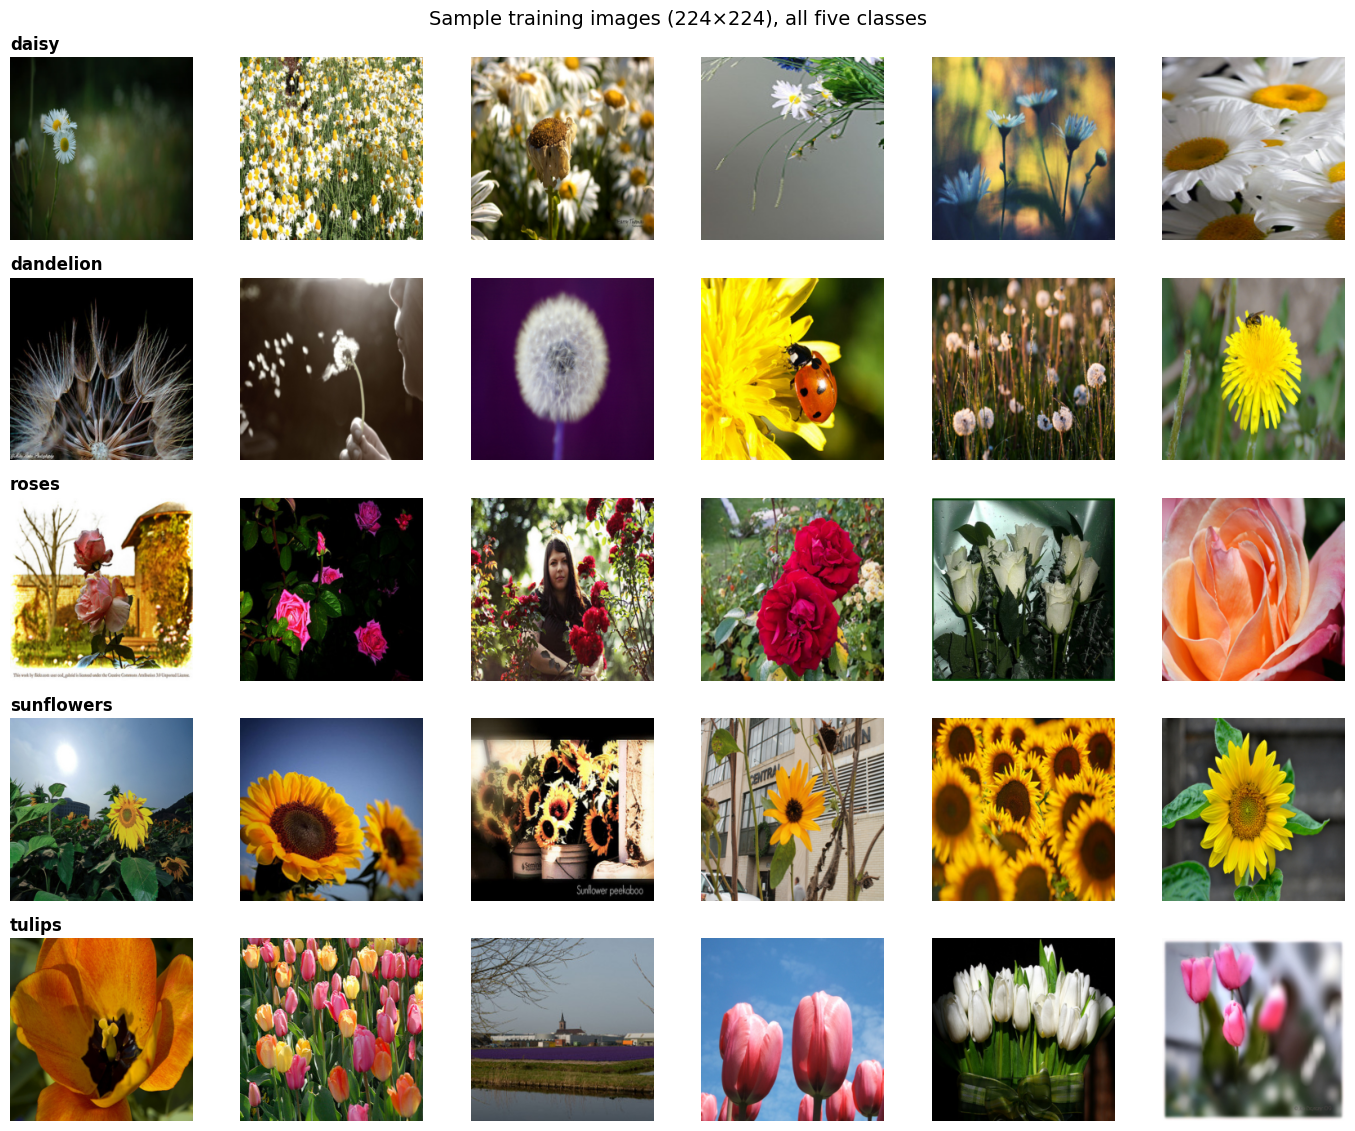
\includegraphics[width=0.85\textwidth]{plots/v01_sample_images.png}
\caption{Sample training images ($224\times224$), six per class.}
\end{figure}

\textbf{Inference:} The six sampled images per class show large within-class variation in scale
(single close-up flower heads versus wide shots of whole fields), viewpoint, illumination
(dark backgrounds, bright sky), and colour (white, pink and yellow tulips; red, pink, white and
orange roses; yellow flowers as well as white seed heads in the dandelion class).
Several images also contain other objects, for example a ladybird on a dandelion flower, a
person among roses and a building behind a sunflower. The classes are
therefore not visually uniform, which makes the dataset suitable for studying where the
network obtains its evidence. The split is moderately imbalanced
(dandelion 898 images versus daisy 633), which is one reason macro F1 is reported next to accuracy.

% ============================================================
\section*{4. Source Code}
% ============================================================

The complete implementation (dataset preparation and the fixed 70:15:15 split, the channel, spatial,
sequential channel--spatial, self-attention, ECA and CBAM modules, the ResNet50 insertion
code, the transfer-learning/fine-tuning pipeline, the five main experiments, the Grad-CAM and
attention-map visualizations and the result tables) is available at the following GitHub
repository:

\begin{center}
\url{https://github.com/PolarFox08/Deep-Learning-Lab/tree/main/Deep%20Learning%20Lab%208}
\end{center}

% ============================================================
\section*{5. Pretrained Architecture: ResNet50}
% ============================================================

ResNet50 pretrained using ImageNet is used as the
\textbf{only backbone architecture} in this experiment.

For an input image

\[
I\in\mathbb{R}^{224\times224\times3},
\]

the major ResNet50 stages produce approximately the following feature
dimensions:

\begin{center}

\begin{tabular}{|l|c|c|}
\hline
\textbf{ResNet50 Stage}
&
\textbf{Spatial Resolution}
&
\textbf{Channels}
\\
\hline

Stem + MaxPool
&
$56\times56$
&
64
\\
\hline

conv2\_x
&
$56\times56$
&
256
\\
\hline

conv3\_x
&
$28\times28$
&
512
\\
\hline

conv4\_x
&
$14\times14$
&
1024
\\
\hline

conv5\_x
&
$7\times7$
&
2048
\\
\hline

\end{tabular}

\end{center}

As the network becomes deeper:

\[
\boxed{
\text{Spatial Resolution}\downarrow
}
\]

while

\[
\boxed{
\text{Feature Channels}\uparrow
}
\]

and the representation generally progresses from low-level visual
information toward higher-level semantic information.

% ============================================================
\section*{6. Understanding ResNet50 Feature Hierarchy}
% ============================================================

The approximate interpretation of different stages is:

\begin{itemize}

\item \textbf{Early features:}
edges, colors, orientations, boundaries, and simple textures.

\item \textbf{Intermediate features:}
local patterns, repeated structures, flower parts, petal arrangements, and
shape information.

\item \textbf{Late features:}
high-level object structures and class-discriminative semantic information.

\end{itemize}

Therefore, the same attention mechanism may produce different behavior when
inserted at different locations.

% ============================================================
\section*{7. Why Attention Position Matters}
% ============================================================

Attention is not independent of the features on which it operates.

Suppose an attention module receives

\[
F\in\mathbb{R}^{H\times W\times C}.
\]

The values of

\[
H,\qquad W,\qquad C
\]

and the semantic meaning of the feature tensor change significantly with
network depth.

Therefore:

\begin{itemize}

\item \textbf{early-stage attention} operates on high-resolution,
low-level visual information;

\item \textbf{middle-stage attention} operates on intermediate features
containing both spatial and semantic information; and

\item \textbf{late-stage attention} operates on low-resolution,
high-level semantic representations.

\end{itemize}

Thus, students should investigate both:

\[
\boxed{\text{Which attention mechanism should be used?}}
\]

and

\[
\boxed{\text{Where should the attention mechanism be inserted?}}
\]

% ============================================================
\section*{8. Candidate Attention Positions}
% ============================================================

Define four candidate attention positions in ResNet50.

\[
P_1:
\text{ after conv2\_x},
\]

\[
P_2:
\text{ after conv3\_x},
\]

\[
P_3:
\text{ after conv4\_x},
\]

\[
P_4:
\text{ after conv5\_x}.
\]

The corresponding feature dimensions are:

\begin{center}

\begin{tabular}{|c|c|c|c|}
\hline

\textbf{Position}
&
\textbf{Location}
&
\textbf{Resolution}
&
\textbf{Channels}
\\
\hline

$P_1$
&
After conv2\_x
&
$56\times56$
&
256
\\
\hline

$P_2$
&
After conv3\_x
&
$28\times28$
&
512
\\
\hline

$P_3$
&
After conv4\_x
&
$14\times14$
&
1024
\\
\hline

$P_4$
&
After conv5\_x
&
$7\times7$
&
2048
\\
\hline

\end{tabular}

\end{center}

For the principal laboratory exercise, students should concentrate on

\[
\boxed{
P_2,\quad P_3,\quad P_4
}
\]

because $P_1$ contains comparatively high-resolution features and may
substantially increase the computational cost of some attention mechanisms.

% ============================================================
\section*{9. Baseline Model}
% ============================================================

The baseline is the pretrained ResNet50 without any additional attention
mechanism.

\begin{center}

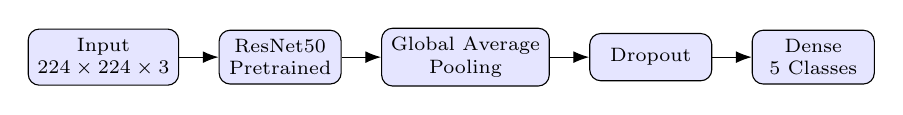
\begin{tikzpicture}[node distance=5mm]

\node[block] (a)
{Input\\$224\times224\times3$};

\node[block,right=of a] (b)
{ResNet50\\Pretrained};

\node[block,right=of b] (c)
{Global Average\\Pooling};

\node[block,right=of c] (d)
{Dropout};

\node[block,right=of d] (e)
{Dense\\5 Classes};

\foreach \x/\y in {a/b,b/c,c/d,d/e}
\draw[arrow] (\x)--(\y);

\end{tikzpicture}

\end{center}

The baseline establishes the reference performance against which the
attention-based models are compared.

% ============================================================
\section*{10. Channel Attention}
% ============================================================

Consider a feature tensor

\[
F\in\mathbb{R}^{H\times W\times C}.
\]

Channel attention determines the relative importance of different feature
channels.

Global average pooling is first used to generate a channel descriptor:

\[
z_c
=
\frac{1}{HW}
\sum_{i=1}^{H}
\sum_{j=1}^{W}
F(i,j,c).
\]

Thus,

\[
z\in\mathbb{R}^{C}.
\]

The channel descriptor is transformed using two learnable transformations:

\[
M_c(F)
=
\sigma
\left(
W_2
\delta
\left(
W_1z
\right)
\right),
\]

where:

\begin{itemize}

\item $\delta(\cdot)$ denotes a nonlinear activation such as ReLU;

\item $\sigma(\cdot)$ denotes the sigmoid activation;

\item $W_1$ reduces the channel representation; and

\item $W_2$ restores the channel dimension.

\end{itemize}

The refined feature tensor is:

\[
F_c
=
F\odot M_c(F).
\]

Channel attention attempts to answer:

\[
\boxed{\text{Which feature channels are important?}}
\]

A reduction ratio of

\[
r=16
\]

may be used as the default setting throughout the laboratory experiment.

The reduction ratio need not be treated as a separate mandatory ablation.

% ============================================================
\section*{11. Spatial Attention}
% ============================================================

Spatial attention determines the spatial regions that should receive greater
importance.

For the input feature tensor

\[
F\in\mathbb{R}^{H\times W\times C},
\]

compute average pooling across channels:

\[
F_{\mathrm{avg}}
=
\operatorname{Mean}_{c}(F),
\]

and maximum pooling across channels:

\[
F_{\mathrm{max}}
=
\operatorname{Max}_{c}(F).
\]

Both tensors have dimensions

\[
H\times W\times1.
\]

Concatenate them:

\[
F_s
=
[
F_{\mathrm{avg}}
\Vert
F_{\mathrm{max}}
].
\]

The spatial attention map is then computed as

\[
M_s(F)
=
\sigma
\left(
\operatorname{Conv}_{7\times7}(F_s)
\right).
\]

Therefore,

\[
M_s(F)
\in
\mathbb{R}^{H\times W\times1}.
\]

The spatially refined feature is

\[
F_s'
=
F\odot M_s(F).
\]

Spatial attention answers:

\[
\boxed{\text{Which spatial locations are important?}}
\]

% ============================================================
\section*{12. Sequential Channel--Spatial Attention}
% ============================================================

Channel and spatial attention can be sequentially applied.

First,

\[
F_c
=
M_c(F)\odot F.
\]

Then,

\[
F_{cs}
=
M_s(F_c)\odot F_c.
\]

The overall structure becomes:

\[
\boxed{
F
\rightarrow
\text{Channel Attention}
\rightarrow
\text{Spatial Attention}
\rightarrow
F_{cs}
}
\]

This arrangement first determines

\[
\text{``what is important''}
\]

and then determines

\[
\text{``where it is important.''}
\]

A simplified diagram is shown below.

\begin{center}

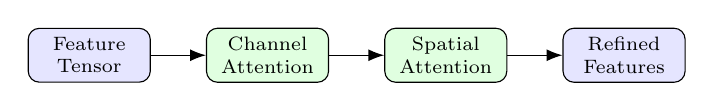
\begin{tikzpicture}[node distance=7mm]

\node[block] (a)
{Feature\\Tensor};

\node[attn,right=of a] (b)
{Channel\\Attention};

\node[attn,right=of b] (c)
{Spatial\\Attention};

\node[block,right=of c] (d)
{Refined\\Features};

\draw[arrow] (a)--(b);
\draw[arrow] (b)--(c);
\draw[arrow] (c)--(d);

\end{tikzpicture}

\end{center}

% ============================================================
\section*{13. Self-Attention}
% ============================================================

Self-attention allows spatial locations to interact directly with other
spatial locations.

For

\[
F\in\mathbb{R}^{H\times W\times C},
\]

flatten the spatial dimensions:

\[
X\in\mathbb{R}^{N\times C},
\]

where

\[
N=HW.
\]

Generate the query, key, and value matrices:

\[
Q=XW_Q,
\]

\[
K=XW_K,
\]

and

\[
V=XW_V.
\]

The attention matrix is

\[
A
=
\operatorname{softmax}
\left(
\frac{QK^T}{\sqrt{d}}
\right),
\]

where $d$ is the dimension of the query/key representation.

The attended output is

\[
Y=AV.
\]

After reshaping the output back to the original spatial structure, a residual
formulation may be used:

\[
F_{\mathrm{SA}}
=
F
+
\gamma
\operatorname{reshape}(Y),
\]

where $\gamma$ is a learnable scaling parameter.

Self-attention attempts to answer:

\[
\boxed{
\text{Which spatial features are related to other spatial features?}
}
\]

Since the attention matrix has dimension approximately

\[
N\times N,
\]

its computational requirements increase rapidly as

\[
N=HW
\]

increases.

Therefore, self-attention should preferably be introduced at

\[
P_3
\]

or

\[
P_4.
\]

% ============================================================
\section*{14. Inserting Attention into ResNet50}
% ============================================================

For any selected stage $P_k$, the network structure can be written as

\[
\text{Previous ResNet Stage}
\rightarrow
\text{Attention}
\rightarrow
\text{Next ResNet Stage}.
\]

For example, attention inserted after conv4\_x gives:

\[
\boxed{
\text{conv4\_x}
\rightarrow
\text{Attention}
\rightarrow
\text{conv5\_x}
}
\]

For channel--spatial attention:

\[
\boxed{
\text{conv4\_x}
\rightarrow
\text{Channel Attention}
\rightarrow
\text{Spatial Attention}
\rightarrow
\text{conv5\_x}
}
\]

The student must record the feature dimensions immediately before and after
the attention block.

Attention should not unintentionally modify the spatial or channel
dimensions unless the selected mechanism explicitly requires such a
transformation.


\textbf{Recorded feature dimensions.} The tensor shapes immediately before and after every attention
block were recorded for all 16 models (format $(H,W,C)$). In every case the output shape is identical to
the input shape, i.e.\ no attention module changed the spatial or channel dimensions.

\begin{center}
\resizebox{\textwidth}{!}{
\begin{tabular}{|c|l|c|l|c|c|}
\hline
\textbf{ID} & \textbf{Model} & \textbf{Position} & \textbf{Module} & \textbf{Input dims} & \textbf{Output dims} \\
\hline
A1 & Channel Attention & P3 & channel & (14,14,1024) & (14,14,1024) \\
\hline
A2 & Spatial Attention ($7\times7$) & P3 & spatial & (14,14,1024) & (14,14,1024) \\
\hline
A3 & Channel+Spatial & P3 & channel $\rightarrow$ spatial & (14,14,1024) & (14,14,1024) \\
\hline
A4 & Self-Attention & P3 & self & (14,14,1024) & (14,14,1024) \\
\hline
A5 & Combined & P3 & channel $\rightarrow$ spatial $\rightarrow$ self & (14,14,1024) & (14,14,1024) \\
\hline
B1 & Channel+Spatial & P1 & channel $\rightarrow$ spatial & (56,56,256) & (56,56,256) \\
\hline
B2 & Channel+Spatial & P2 & channel $\rightarrow$ spatial & (28,28,512) & (28,28,512) \\
\hline
B4 & Channel+Spatial & P4 & channel $\rightarrow$ spatial & (7,7,2048) & (7,7,2048) \\
\hline
C1 & Channel+Spatial & P3 & channel $\rightarrow$ spatial & (14,14,1024) & (14,14,1024) \\
\hline
C1 & Channel+Spatial & P4 & channel $\rightarrow$ spatial & (7,7,2048) & (7,7,2048) \\
\hline
C2 & Channel+Spatial & P2 & channel $\rightarrow$ spatial & (28,28,512) & (28,28,512) \\
\hline
C2 & Channel+Spatial & P3 & channel $\rightarrow$ spatial & (14,14,1024) & (14,14,1024) \\
\hline
C2 & Channel+Spatial & P4 & channel $\rightarrow$ spatial & (7,7,2048) & (7,7,2048) \\
\hline
D1 & Spatial$\rightarrow$Channel & P3 & spatial $\rightarrow$ channel & (14,14,1024) & (14,14,1024) \\
\hline
E1 & Spatial Attention ($3\times3$) & P3 & spatial & (14,14,1024) & (14,14,1024) \\
\hline
E2 & Spatial Attention ($5\times5$) & P3 & spatial & (14,14,1024) & (14,14,1024) \\
\hline
F1 & ECA & P3 & eca & (14,14,1024) & (14,14,1024) \\
\hline
F2 & CBAM & P3 & channel $\rightarrow$ spatial & (14,14,1024) & (14,14,1024) \\
\hline
\end{tabular}}
\end{center}

\textbf{Inference:} All attention modules are shape-preserving ($H\times W\times C$ unchanged) at all four candidate
positions: $56\times56\times256$ ($P_1$), $28\times28\times512$ ($P_2$), $14\times14\times1024$ ($P_3$) and
$7\times7\times2048$ ($P_4$). The pretrained stages that follow an attention block can therefore be
used unchanged, and the only difference between models is the re-weighting performed by the module.

% ============================================================
\section*{15. Main Experiment 1: Attention-Type Ablation}
% ============================================================

The first experiment studies the effect of different types of attention.

Fix the attention position at

\[
\boxed{
P_3=\text{after conv4\_x}
}
\]

for all models.

Compare the following:

\begin{center}

\begin{tabular}{|l|c|c|c|}
\hline

\textbf{Model}
&
\textbf{Channel}
&
\textbf{Spatial}
&
\textbf{Self-Attention}
\\
\hline

A0: Baseline ResNet50
&
--
&
--
&
--
\\
\hline

A1: Channel Attention
&
$\checkmark$
&
--
&
--
\\
\hline

A2: Spatial Attention
&
--
&
$\checkmark$
&
--
\\
\hline

A3: Channel+Spatial
&
$\checkmark$
&
$\checkmark$
&
--
\\
\hline

A4: Self-Attention
&
--
&
--
&
$\checkmark$
\\
\hline

A5: Combined Attention
&
$\checkmark$
&
$\checkmark$
&
$\checkmark$
\\
\hline

\end{tabular}

\end{center}

This experiment investigates:

\[
\boxed{
\text{How does attention type affect model performance?}
}
\]

Students must keep the following identical:

\begin{itemize}

\item dataset split;

\item preprocessing;

\item augmentation;

\item optimizer;

\item learning rate schedule;

\item epochs;

\item batch size;

\item backbone;

\item classifier;

\item attention position; and

\item evaluation procedure.

\end{itemize}


\subsection*{Results}

All six models use the identical protocol (see Section 21 for the configuration), with the
attention module inserted at $P_3$. Test set: 551 images.

\begin{center}
\resizebox{\textwidth}{!}{
\begin{tabular}{|l|c|c|c|c|r|r|c|c|}
\hline
\textbf{Model} & \textbf{Acc.} & \textbf{Prec.} & \textbf{Recall} & \textbf{Macro F1} & \textbf{Total Params} & \textbf{Attn. Params} & \textbf{Train (s)} & \textbf{Infer. (ms/img)} \\
\hline
A0: Baseline ResNet50 & 0.9510 & 0.9519 & 0.9503 & 0.9509 & 23{,}597{,}957 & 0 & 343.2 & 3.904 \\
\hline
A1: Channel Attention (SE-style) & 0.9456 & 0.9455 & 0.9473 & 0.9457 & 23{,}730{,}117 & 132{,}160 & 338.9 & 3.962 \\
\hline
A2: Spatial Attention ($7\times7$) & 0.9165 & 0.9200 & 0.9170 & 0.9181 & 23{,}598{,}056 & 99 & 337.6 & 3.953 \\
\hline
A3: Channel+Spatial (C$\rightarrow$S) & 0.9292 & 0.9302 & 0.9278 & 0.9284 & 23{,}730{,}216 & 132{,}259 & 340.4 & 3.962 \\
\hline
A4: Self-Attention & 0.9437 & 0.9507 & 0.9410 & 0.9444 & 24{,}908{,}678 & 1{,}310{,}721 & 348.0 & 4.243 \\
\hline
A5: Combined (C$\rightarrow$S$\rightarrow$Self) & 0.9201 & 0.9191 & 0.9221 & 0.9199 & 25{,}040{,}937 & 1{,}442{,}980 & 356.0 & 4.276 \\
\hline
\end{tabular}}
\end{center}

\textbf{Complexity and measured qualitative statistics.} Trainable parameters refer to the
fine-tuning stage ($\texttt{conv5\_x}$ unfrozen). Grad-CAM coverage is the fraction of the
$224\times224$ map with value $\ge0.5$ and entropy is the normalised Shannon entropy of the
$7\times7$ Grad-CAM map (both averaged over the whole test set).

\begin{center}
\resizebox{\textwidth}{!}{
\begin{tabular}{|l|r|c|c|}
\hline
\textbf{Model} & \textbf{Trainable Params (fine-tune)} & \textbf{Grad-CAM Cov.} & \textbf{Grad-CAM Entropy} \\
\hline
A0: Baseline ResNet50 & 14{,}963{,}717 & 0.2354 & 0.8422 \\
\hline
A1: Channel Attention (SE-style) & 15{,}095{,}877 & 0.2099 & 0.8265 \\
\hline
A2: Spatial Attention ($7\times7$) & 14{,}963{,}816 & 0.1798 & 0.8175 \\
\hline
A3: Channel+Spatial (C$\rightarrow$S) & 15{,}095{,}976 & 0.2028 & 0.8244 \\
\hline
A4: Self-Attention & 16{,}274{,}438 & 0.2738 & 0.8876 \\
\hline
A5: Combined (C$\rightarrow$S$\rightarrow$Self) & 16{,}406{,}697 & 0.3065 & 0.9014 \\
\hline
\end{tabular}}
\end{center}

\begin{center}
\small
\begin{tabular}{|l|p{12cm}|}
\hline
\textbf{Model} & \textbf{Internal attention-map statistics (test set)} \\
\hline
A1 & P3 channel: mean 0.590, std 0.427 \\
\hline
A2 & P3 spatial: mean 0.885, std 0.264, $>$0.5: 87.3\% \\
\hline
A3 & P3 channel: mean 0.613, std 0.405; P3 spatial: mean 0.986, std 0.043, $>$0.5: 99.9\% \\
\hline
A4 & P3 self: row-entropy 0.010, mean distance 6.35 cells (uniform: 7.28) \\
\hline
A5 & P3 channel: mean 0.551, std 0.333; P3 spatial: mean 0.954, std 0.115, $>$0.5: 98.0\%; P3 self: row-entropy 0.024, distance 6.43 (uniform: 7.28) \\
\hline
\end{tabular}
\end{center}

\textbf{Inference:} The \textbf{baseline} ResNet50 obtained the highest test accuracy (0.9510, 524 of 551 images correct) and
macro F1 (0.9509); none of the attention variants exceeded it. Ranked by test accuracy the attention
models were: channel (SE-style) 0.9456, self-attention 0.9437, channel+spatial 0.9292, combined 0.9201 and
spatial 0.9165 (505 correct, the lowest, $-3.45$ percentage points relative to the baseline). The gaps between the baseline,
channel attention and self-attention are 3--4 test images, which is below the sampling noise of a single run (the
binomial standard error of an accuracy near 0.95 on 551 images is roughly 0.9 percentage points), so these three
should be regarded as comparable; the lower accuracy of spatial, channel+spatial and combined attention is larger.
\textbf{Complexity:} the channel module adds 132{,}160 parameters (0.56\% of the baseline) and
$+0.058$ ms per image (3.962 vs.\ 3.904 ms); the spatial module adds only 99 parameters; self-attention adds
1{,}310{,}721 parameters ($+5.6\%$) and $+0.339$ ms ($+8.7\%$); the combined module adds 1{,}442{,}980 parameters and
$+0.372$ ms. Training time differs by at most 13 s (338--356 s).
\textbf{Qualitative statistics:} the spatial maps are almost saturated (mean 0.885 for spatial-only; 0.986 with 99.9\% of
positions above 0.5 when preceded by channel attention), the channel weights are bimodal (mean 0.59, std 0.43), and the
self-attention rows are extremely peaked (normalised row entropy 0.010; learned residual scale $\gamma=0.0611$).
Grad-CAM coverage is lower than the baseline (0.2354) for channel (0.2099), spatial (0.1798) and channel+spatial (0.2028)
attention, but higher for self-attention (0.2738) and the combined module (0.3065).
The training-behaviour columns (Section 39) show that self-attention and channel attention reach 90\% validation accuracy earlier
than the baseline (epoch 2 and 3 versus 6; the baseline's validation accuracy was printed as 0.9000 at epochs 4--5, which is borderline for the
strict $\ge0.90$ criterion), and that self-attention has the lowest test loss (0.1542 versus 0.1875 for the baseline) even though its
accuracy is 0.73 percentage points lower.

% ============================================================
\section*{16. Main Experiment 2: Attention-Position Ablation}
% ============================================================

The second experiment investigates the influence of the position of
attention.

Fix the attention type as:

\[
\boxed{
\text{Channel Attention}
\rightarrow
\text{Spatial Attention}
}
\]

and insert exactly the same module at different stages.

\begin{center}

\begin{tabular}{|l|l|c|c|}
\hline

\textbf{Experiment}
&
\textbf{Attention Position}
&
\textbf{Resolution}
&
\textbf{Channels}
\\
\hline

B1
&
After conv2\_x
&
$56\times56$
&
256
\\
\hline

B2
&
After conv3\_x
&
$28\times28$
&
512
\\
\hline

B3
&
After conv4\_x
&
$14\times14$
&
1024
\\
\hline

B4
&
After conv5\_x
&
$7\times7$
&
2048
\\
\hline

\end{tabular}

\end{center}

Students should study whether attention is more beneficial for:

\begin{itemize}

\item high-resolution low-level features;

\item intermediate representations; or

\item low-resolution semantic features.

\end{itemize}

The principal question is:

\[
\boxed{
\text{How does the location of attention influence performance?}
}
\]


\subsection*{Results}

The same Channel$\rightarrow$Spatial module ($r=16$, $7\times7$ kernel) was inserted at each position.
B3 is the same model as A3 and was reused.

\begin{center}
\resizebox{\textwidth}{!}{
\begin{tabular}{|l|c|c|c|c|c|c|c|r|r|c|}
\hline
\textbf{Exp.} & \textbf{Pos.} & \textbf{Res.} & \textbf{Ch.} & \textbf{Acc.} & \textbf{Prec.} & \textbf{Recall} & \textbf{F1} & \textbf{Total Params} & \textbf{Attn. Params} & \textbf{Infer. (ms)} \\
\hline
B1 & P1 & $56\times56$ & 256 & 0.9111 & 0.9224 & 0.9062 & 0.9122 & 23{,}606{,}520 & 8{,}563 & 4.171 \\
\hline
B2 & P2 & $28\times28$ & 512 & 0.9419 & 0.9418 & 0.9417 & 0.9416 & 23{,}631{,}368 & 33{,}411 & 4.046 \\
\hline
B3 (= A3) & P3 & $14\times14$ & 1024 & 0.9292 & 0.9302 & 0.9278 & 0.9284 & 23{,}730{,}216 & 132{,}259 & 3.962 \\
\hline
B4 & P4 & $7\times7$ & 2048 & 0.9492 & 0.9499 & 0.9501 & 0.9499 & 24{,}124{,}520 & 526{,}563 & 3.981 \\
\hline
\end{tabular}}
\end{center}

\begin{center}
\small
\begin{tabular}{|l|c|c|p{9.2cm}|}
\hline
\textbf{Model} & \textbf{Grad-CAM Cov.} & \textbf{Grad-CAM Entropy} & \textbf{Internal attention-map statistics (test set)} \\
\hline
B1 ($P_1$) & 0.1841 & 0.8207 & P1 channel: mean 0.628, std 0.317; P1 spatial: mean 0.978, std 0.067, $>$0.5: 99.4\% \\
\hline
B2 ($P_2$) & 0.1935 & 0.8080 & P2 channel: mean 0.635, std 0.389; P2 spatial: mean 0.978, std 0.090, $>$0.5: 98.7\% \\
\hline
B3 = A3 ($P_3$) & 0.2028 & 0.8244 & P3 channel: mean 0.613, std 0.405; P3 spatial: mean 0.986, std 0.043, $>$0.5: 99.9\% \\
\hline
B4 ($P_4$) & 0.2499 & 0.9032 & P4 channel: mean 0.483, std 0.369; P4 spatial: mean 0.990, std 0.038, $>$0.5: 99.6\% \\
\hline
\end{tabular}
\end{center}

\begin{figure}[H]
\centering
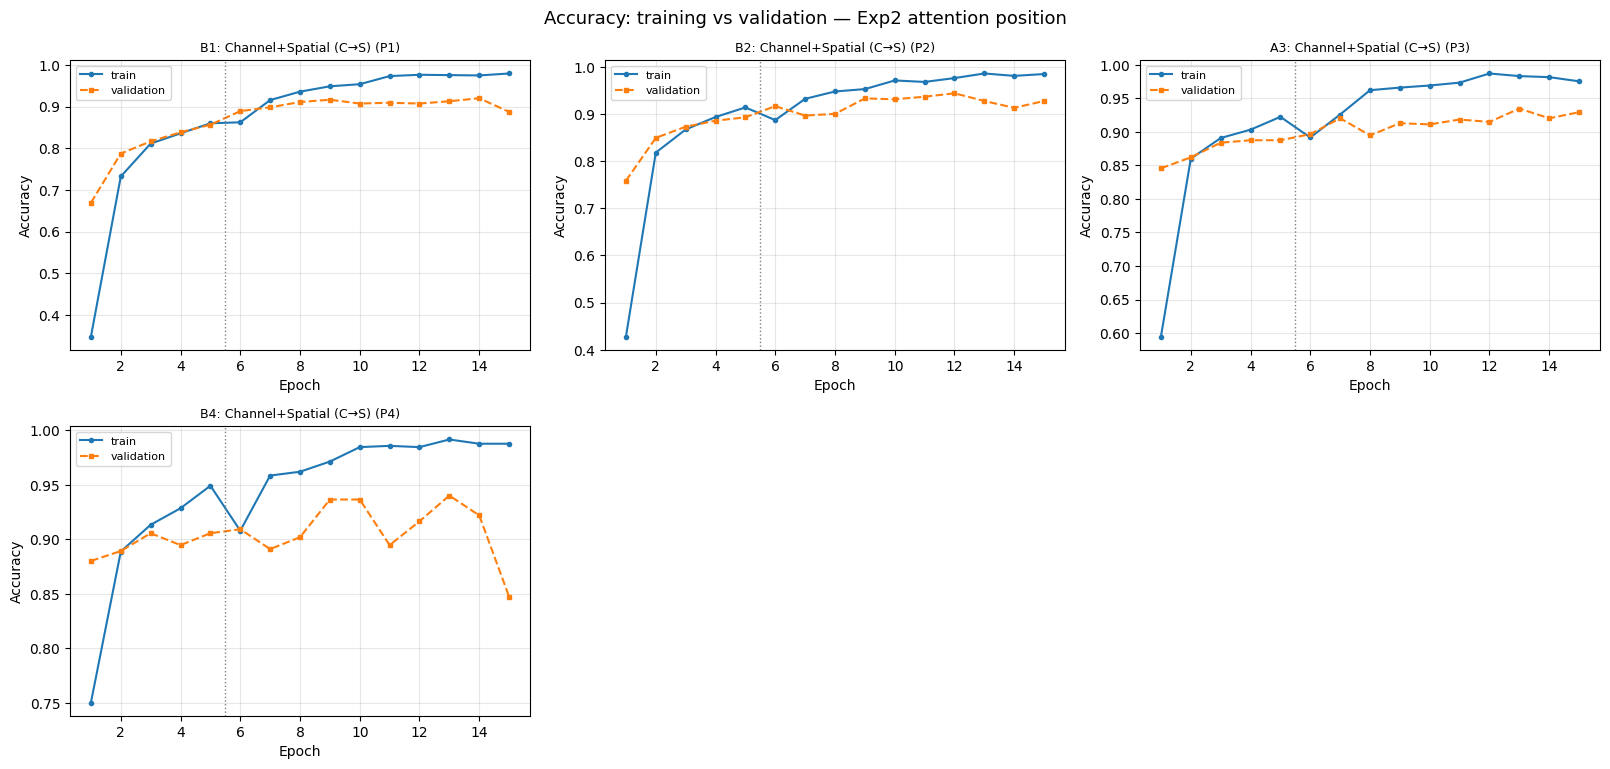
\includegraphics[width=0.95\textwidth]{plots/v_curves_accuracy_exp2.png}
\caption{Training and validation accuracy of the position-ablation models (Experiment 2). The dotted vertical line marks the start of fine-tuning.}
\end{figure}

\begin{figure}[H]
\centering
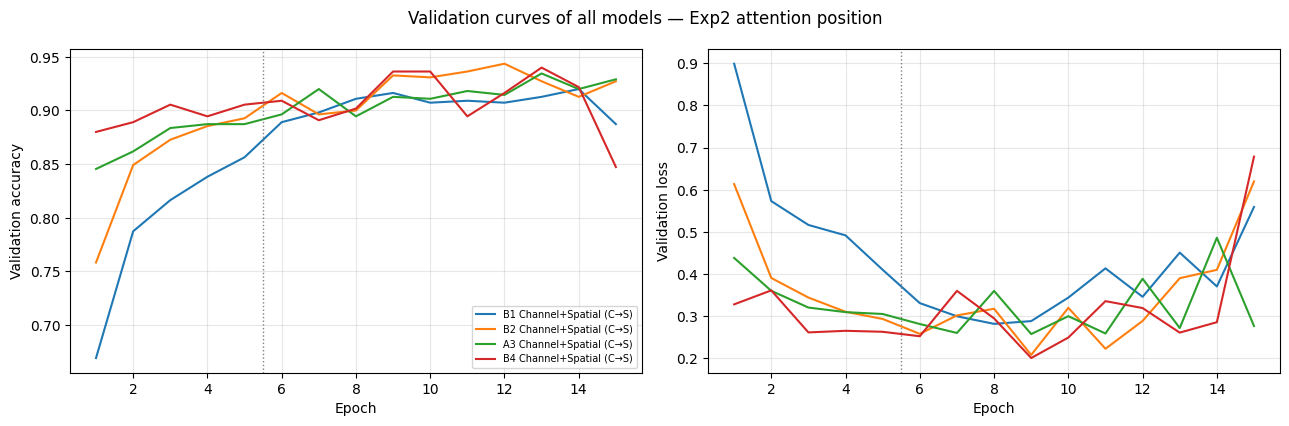
\includegraphics[width=0.90\textwidth]{plots/v_curves_val_overlay_exp2.png}
\caption{Validation accuracy and validation loss of B1--B4 overlaid.}
\end{figure}

\textbf{Inference:} Attention position clearly affected accuracy: $P_1$ (after \texttt{conv2\_x}) gave the lowest test accuracy (0.9111, $-3.99$ points
relative to the baseline), $P_2$ 0.9419, $P_3$ 0.9292 and $P_4$ (after \texttt{conv5\_x}) the highest (0.9492, only one image below the baseline's 0.9510).
The trend is not monotonic ($P_3$ is below $P_2$), but the shallowest position was worst and the deepest best. Complexity behaves differently from
accuracy: the module's parameter count grows with depth because the channel MLP scales with $C$ (8{,}563 at $P_1$, 33{,}411 at $P_2$, 132{,}259 at $P_3$ and 526{,}563 at $P_4$), whereas
the inference time is highest at $P_1$ (4.171 ms, $+6.8\%$ over the baseline) because the maps are $56\times56$, and lowest at $P_3$ (3.962 ms).
The curves show that $P_1$ learns slowest (validation accuracy after epoch 1: 0.669 versus 0.758 at $P_2$, 0.846 at $P_3$ and 0.880 at $P_4$; first epoch with
$\ge0.90$ validation accuracy: 8 versus 6, 7 and 3). $P_4$'s validation accuracy and loss deteriorate sharply in the last epoch (to about 0.85 and 0.68), but the weights of the
lowest-validation-loss epoch (epoch 9) were restored before testing. The spatial maps are almost saturated at every position (mean 0.978, 0.978, 0.986 and 0.990 for $P_1$--$P_4$), while the
mean channel weight is lowest at the deepest stage (0.483 at $P_4$ versus 0.613--0.635 elsewhere). Grad-CAM coverage grows with depth (0.184, 0.194, 0.203, 0.250) and $P_4$ has the most diffuse Grad-CAM
(entropy 0.903) while giving the best accuracy, so a more compact Grad-CAM was not associated with higher accuracy in this experiment.

% ============================================================
\section*{17. Main Experiment 3: Multiple Attention Positions}
% ============================================================

Attention may also be inserted at more than one ResNet50 stage.

Compare:

\[
\text{Attention only at }P_3,
\]

\[
\text{Attention only at }P_4,
\]

and

\[
\text{Attention at }P_3+P_4.
\]

As an extended experiment, students may evaluate:

\[
P_2+P_3+P_4.
\]

The purpose is to investigate whether applying attention repeatedly provides
sufficient performance improvement to justify the additional:

\begin{itemize}

\item parameters;

\item computation;

\item memory;

\item training time; and

\item inference time.

\end{itemize}

Students should experimentally answer:

\[
\boxed{
\text{Is attention at more locations necessarily more effective?}
}
\]


\subsection*{Results}

\begin{center}
\resizebox{\textwidth}{!}{
\begin{tabular}{|l|c|c|c|c|r|r|c|c|}
\hline
\textbf{Positions} & \textbf{Acc.} & \textbf{Prec.} & \textbf{Recall} & \textbf{F1} & \textbf{Total Params} & \textbf{Attn. Params} & \textbf{Train (s)} & \textbf{Infer. (ms)} \\
\hline
$P_3$ only & 0.9292 & 0.9302 & 0.9278 & 0.9284 & 23{,}730{,}216 & 132{,}259 & 340.4 & 3.962 \\
\hline
$P_4$ only & 0.9492 & 0.9499 & 0.9501 & 0.9499 & 24{,}124{,}520 & 526{,}563 & 340.3 & 3.981 \\
\hline
$P_3+P_4$ & 0.9328 & 0.9346 & 0.9333 & 0.9336 & 24{,}256{,}779 & 658{,}822 & 346.8 & 4.009 \\
\hline
$P_2+P_3+P_4$ & 0.9256 & 0.9273 & 0.9264 & 0.9258 & 24{,}290{,}190 & 692{,}233 & 359.7 & 4.075 \\
\hline
\end{tabular}}
\end{center}

Difference with respect to $P_3$ only (value $-$ value of $P_3$ only):

\begin{center}
\begin{tabular}{|l|c|c|c|c|c|}
\hline
\textbf{Positions} & \textbf{$\Delta$ Acc.} & \textbf{$\Delta$ F1} & \textbf{$\Delta$ Attn. Params} & \textbf{$\Delta$ Train (s)} & \textbf{$\Delta$ Infer. (ms)} \\
\hline
$P_4$ only & +0.0200 & +0.0215 & +394{,}304 & $-0.1$ & +0.019 \\
\hline
$P_3+P_4$ & +0.0036 & +0.0052 & +526{,}563 & +6.4 & +0.047 \\
\hline
$P_2+P_3+P_4$ & $-0.0036$ & $-0.0026$ & +559{,}974 & +19.3 & +0.113 \\
\hline
\end{tabular}
\end{center}

\begin{center}
\small
\begin{tabular}{|l|c|c|p{9.2cm}|}
\hline
\textbf{Model} & \textbf{Grad-CAM Cov.} & \textbf{Grad-CAM Entropy} & \textbf{Internal attention-map statistics (test set)} \\
\hline
$P_3$ only & 0.2028 & 0.8244 & P3 channel: mean 0.613, std 0.405; P3 spatial: mean 0.986, std 0.043, $>$0.5: 99.9\% \\
\hline
$P_4$ only & 0.2499 & 0.9032 & P4 channel: mean 0.483, std 0.369; P4 spatial: mean 0.990, std 0.038, $>$0.5: 99.6\% \\
\hline
$P_3+P_4$ & 0.2399 & 0.8710 & P3 channel: mean 0.594, std 0.422; P3 spatial: mean 0.992, std 0.030, $>$0.5: 100.0\%; P4 channel: mean 0.509, std 0.383 (remaining entries truncated in the notebook display) \\
\hline
$P_2+P_3+P_4$ & 0.2117 & 0.8511 & P2 channel: mean 0.598, std 0.370; P2 spatial: mean 0.991, std 0.042, $>$0.5: 99.9\%; P3 channel: mean 0.591, std 0.403 (remaining entries truncated in the notebook display) \\
\hline
\end{tabular}
\end{center}

\textbf{Inference:} Attention at more locations was \textbf{not} more effective. Attention at $P_4$ alone (0.9492) outperformed $P_3+P_4$ (0.9328, 9 fewer correct test images)
and $P_2+P_3+P_4$ (0.9256), while using fewer attention parameters (526{,}563 versus 658{,}822 and 692{,}233) and less inference time (3.981 versus 4.009 and 4.075 ms per image).
Relative to $P_3$ only, adding $P_4$ gave a small gain (+0.36 points, within noise) and adding $P_2$ and $P_4$ gave a small loss, in both cases with additional parameters, longer training
(up to +19.3 s) and longer inference (up to +0.113 ms). The multi-position models did not converge faster than the single-position $P_4$ model (first epoch with validation accuracy $\ge0.90$: 3, 3 and 7 for
$P_4$, $P_3+P_4$ and $P_2+P_3+P_4$), although $P_3+P_4$ had a much smoother validation loss (roughness 0.041 versus 0.075 for $P_4$ only). In this experiment the extra attention parameters, computation
and training time were not justified by the accuracy obtained.

% ============================================================
\section*{18. Main Experiment 4: Attention Order}
% ============================================================

The sequence in which channel and spatial attention are applied may influence
the resulting features.

Compare:

\[
\boxed{
\text{Channel}
\rightarrow
\text{Spatial}
}
\]

against

\[
\boxed{
\text{Spatial}
\rightarrow
\text{Channel}
}
\]

while maintaining the same insertion position.

For example, at $P_3$:

\[
F
\rightarrow
M_c
\rightarrow
M_s
\]

should be compared with

\[
F
\rightarrow
M_s
\rightarrow
M_c.
\]

Students should determine whether selecting informative feature channels
before selecting spatial regions produces behavior different from selecting
spatial regions first.


\subsection*{Results}

Both models insert the module at $P_3$ and have identical parameter counts.

\begin{center}
\resizebox{\textwidth}{!}{
\begin{tabular}{|l|c|c|c|c|r|c|c|c|}
\hline
\textbf{Order} & \textbf{Acc.} & \textbf{Prec.} & \textbf{Recall} & \textbf{F1} & \textbf{Total Params} & \textbf{Infer. (ms)} & \textbf{Grad-CAM Cov.} & \textbf{Grad-CAM Entropy} \\
\hline
Channel $\rightarrow$ Spatial & 0.9292 & 0.9302 & 0.9278 & 0.9284 & 23{,}730{,}216 & 3.962 & 0.2028 & 0.8244 \\
\hline
Spatial $\rightarrow$ Channel & 0.9492 & 0.9525 & 0.9474 & 0.9489 & 23{,}730{,}216 & 3.982 & 0.2224 & 0.8344 \\
\hline
\end{tabular}}
\end{center}

\begin{center}
\small
\begin{tabular}{|l|p{12cm}|}
\hline
\textbf{Order} & \textbf{Internal attention-map statistics (test set)} \\
\hline
Channel $\rightarrow$ Spatial & P3 channel: mean 0.613, std 0.405; P3 spatial: mean 0.986, std 0.043, $>$0.5: 99.9\% \\
\hline
Spatial $\rightarrow$ Channel & P3 spatial: mean 0.936, std 0.169, $>$0.5: 94.8\%; P3 channel: mean 0.631, std 0.420 \\
\hline
\end{tabular}
\end{center}

\textbf{Inference:} Spatial$\rightarrow$Channel (0.9492, macro F1 0.9489) was 2.00 percentage points more accurate than Channel$\rightarrow$Spatial (0.9292, macro F1 0.9284), i.e.\ 523 versus 512 correct test images,
although both models have exactly the same number of parameters (23{,}730{,}216) and nearly the same inference time (3.982 versus 3.962 ms). The order therefore changed the learned behaviour: when the spatial module sees the raw
$P_3$ features first its map is noticeably less saturated (mean 0.936, std 0.169, 94.8\% of positions above 0.5), whereas after channel attention the spatial map is almost constant (mean 0.986, std 0.043, 99.9\% above 0.5).
The Grad-CAM statistics of S$\rightarrow$C are slightly broader (coverage 0.2224 versus 0.2028). Because only one training run per model was performed, the 2-point difference should be confirmed with additional seeds before
concluding that the order always matters.

% ============================================================
\section*{19. Main Experiment 5: Spatial Attention Kernel Size}
% ============================================================

The receptive field used to generate the spatial attention map may influence
the result.

Evaluate:

\[
k\in\{3,5,7\}.
\]

Use the same attention position and training protocol.

\begin{center}

\begin{tabular}{|c|c|c|c|}
\hline

\textbf{Spatial Kernel}
&
\textbf{Accuracy}
&
\textbf{Macro F1}
&
\textbf{Inference Time}
\\
\hline

$3\times3$
&
0.9492
&
0.9500
&
3.951 ms
\\
\hline

$5\times5$
&
0.9274
&
0.9266
&
3.964 ms
\\
\hline

$7\times7$
&
0.9165
&
0.9181
&
3.953 ms
\\
\hline

\end{tabular}

\end{center}

Students should discuss whether a larger spatial kernel provides a useful
increase in contextual information.


\textbf{Additional measurements} (spatial attention only, at $P_3$; the $7\times7$ model is A2):

\begin{center}
\resizebox{\textwidth}{!}{
\begin{tabular}{|c|c|c|r|r|c|c|c|}
\hline
\textbf{Kernel} & \textbf{Prec.} & \textbf{Recall} & \textbf{Total Params} & \textbf{Attn. Params} & \textbf{Train (s)} & \textbf{Grad-CAM Cov.} & \textbf{Grad-CAM Entropy} \\
\hline
$3\times3$ & 0.9490 & 0.9517 & 23{,}597{,}976 & 19 & 340.6 & 0.1945 & 0.8403 \\
\hline
$5\times5$ & 0.9293 & 0.9291 & 23{,}598{,}008 & 51 & 341.6 & 0.1676 & 0.8193 \\
\hline
$7\times7$ & 0.9200 & 0.9170 & 23{,}598{,}056 & 99 & 337.6 & 0.1798 & 0.8175 \\
\hline
\end{tabular}}
\end{center}

\begin{center}
\small
\begin{tabular}{|c|p{12cm}|}
\hline
\textbf{Kernel} & \textbf{Spatial attention-map statistics (test set)} \\
\hline
$3\times3$ & P3 spatial: mean 0.983, std 0.034, $>$0.5: 99.9\% \\
\hline
$5\times5$ & P3 spatial: mean 0.903, std 0.235, $>$0.5: 91.4\% \\
\hline
$7\times7$ & P3 spatial: mean 0.885, std 0.264, $>$0.5: 87.3\% \\
\hline
\end{tabular}
\end{center}

\textbf{Inference:} A larger spatial kernel did \textbf{not} give a useful increase in contextual information here: test accuracy decreased monotonically with kernel size
($3\times3$: 0.9492, $5\times5$: 0.9274, $7\times7$: 0.9165; macro F1 0.9500, 0.9266, 0.9181), while the inference time was practically identical
(3.951, 3.964 and 3.953 ms; differences of about 0.01 ms are not meaningful) and the module remains tiny (19, 51 and 99 parameters). The spatial maps become less saturated as the kernel grows
(mean 0.983, 0.903, 0.885; fraction of positions above 0.5: 99.9\%, 91.4\%, 87.3\%), i.e.\ larger kernels suppress more of the image, and this coincided with lower accuracy. The $3\times3$ spatial model is within one image of the baseline (523 versus 524 correct).

% ============================================================
\section*{20. Additional Task: Comparison of Different Attention Mechanisms}
% ============================================================

As an additional exploration task, students should compare the attention
mechanisms implemented in the laboratory with established attention
approaches.

Students should select at least

\[
\boxed{\text{two additional attention mechanisms}}
\]

from the following:

\begin{itemize}

\item Squeeze-and-Excitation (SE) Attention;

\item Efficient Channel Attention (ECA);

\item Convolutional Block Attention Module (CBAM);

\item Coordinate Attention; and

\item lightweight Self-Attention.

\end{itemize}

The pretrained backbone must remain:

\[
\boxed{\text{ResNet50}}
\]

for all comparisons.

To ensure a fair comparison, additional attention mechanisms should
preferably be inserted at the same position:

\[
\boxed{
P_3=\text{after conv4\_x}
}
\]

unless the student provides a technical justification for using another
location.

% ============================================================
\subsection*{20.1 Suggested Comparison}
% ============================================================

\begin{center}

\resizebox{\textwidth}{!}{
\begin{tabular}{|l|c|c|c|c|c|c|}
\hline

\textbf{Attention}
&
\textbf{Accuracy}
&
\textbf{Precision}
&
\textbf{Recall}
&
\textbf{Macro F1}
&
\textbf{Parameters}
&
\textbf{Inference Time}
\\
\hline

No Attention
&
0.9510
&
0.9519
&
0.9503
&
0.9509
&
23{,}597{,}957
&
3.904 ms
\\
\hline

Channel / SE
&
0.9456
&
0.9455
&
0.9473
&
0.9457
&
23{,}730{,}117
&
3.962 ms
\\
\hline

Spatial Attention
&
0.9165
&
0.9200
&
0.9170
&
0.9181
&
23{,}598{,}056
&
3.953 ms
\\
\hline

ECA
&
0.9220
&
0.9228
&
0.9209
&
0.9213
&
23{,}597{,}962
&
3.942 ms
\\
\hline

CBAM
&
0.9183
&
0.9158
&
0.9220
&
0.9177
&
23{,}730{,}216
&
3.990 ms
\\
\hline

Self-Attention
&
0.9437
&
0.9507
&
0.9410
&
0.9444
&
24{,}908{,}678
&
4.243 ms
\\
\hline

Additional Mechanism (Combined C$\rightarrow$S$\rightarrow$Self, A5)
&
0.9201
&
0.9191
&
0.9221
&
0.9199
&
25{,}040{,}937
&
4.276 ms
\\
\hline

\end{tabular}}
\end{center}


All mechanisms were inserted at $P_3$ with ResNet50 as backbone and the identical protocol. The SE row is the channel-attention
module (global average pooling followed by two fully connected layers with $r=16$, which is exactly the Squeeze-and-Excitation design); the lightweight self-attention row is A4. ECA uses a 1-D convolution over the channel descriptor
(adaptive kernel size 5 for $C=1024$). CBAM combines channel attention (average- and max-pooled descriptors through a shared MLP) with $7\times7$ spatial attention. Coordinate attention was not implemented;
the ``Additional Mechanism'' row therefore reports the combined Channel$\rightarrow$Spatial$\rightarrow$Self-Attention model.

\begin{center}
\begin{tabular}{|l|r|c|c|}
\hline
\textbf{Attention} & \textbf{Attn. Params} & \textbf{Grad-CAM Cov.} & \textbf{Grad-CAM Entropy} \\
\hline
No Attention & 0 & 0.2354 & 0.8422 \\
\hline
Channel / SE & 132{,}160 & 0.2099 & 0.8265 \\
\hline
Spatial Attention & 99 & 0.1798 & 0.8175 \\
\hline
ECA & 5 & 0.1919 & 0.8154 \\
\hline
CBAM & 132{,}259 & 0.1816 & 0.8015 \\
\hline
Self-Attention & 1{,}310{,}721 & 0.2738 & 0.8876 \\
\hline
Additional Mechanism & 1{,}442{,}980 & 0.3065 & 0.9014 \\
\hline
\end{tabular}
\end{center}

\begin{figure}[H]
\centering
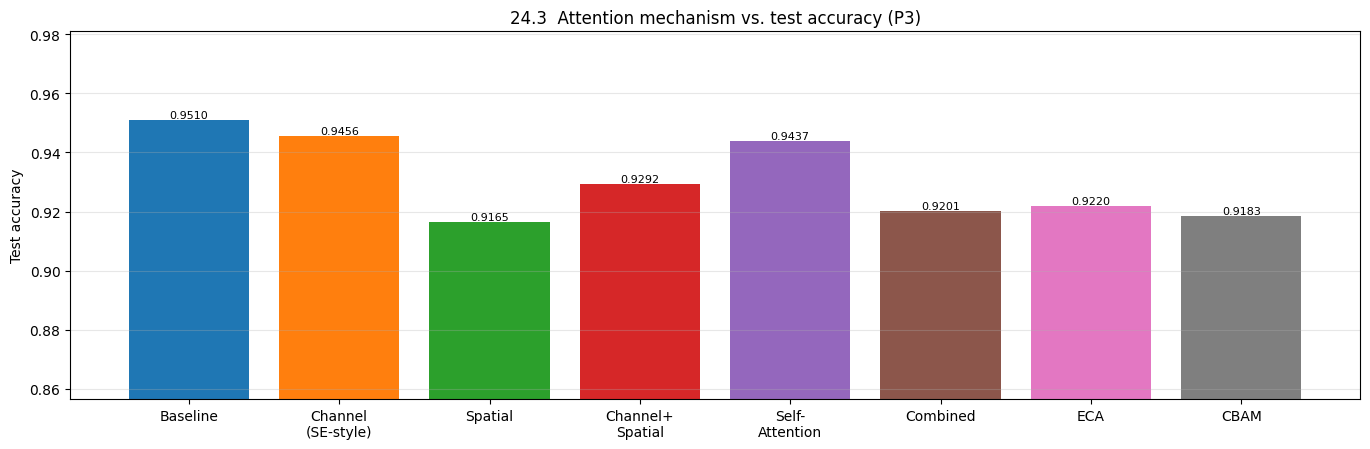
\includegraphics[width=0.90\textwidth]{plots/v_bar_mech_accuracy.png}
\caption{Attention mechanism versus test accuracy (all at $P_3$).}
\end{figure}

\begin{figure}[H]
\centering
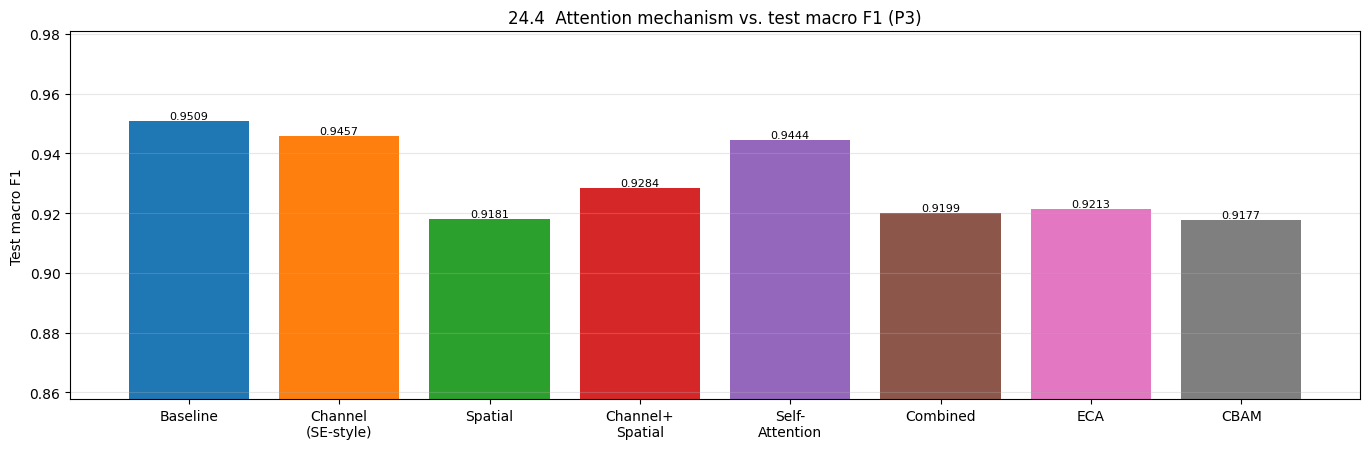
\includegraphics[width=0.90\textwidth]{plots/v_bar_mech_f1.png}
\caption{Attention mechanism versus test macro F1 (all at $P_3$).}
\end{figure}

% ============================================================
\subsection*{20.2 Questions for Attention-Mechanism Comparison}
% ============================================================

Students should investigate:

\begin{enumerate}

\item How does classification accuracy vary across attention mechanisms?

\item How does macro F1-score vary across attention mechanisms?

\item How many parameters are introduced by each attention module?

\item How does each attention mechanism influence inference time?

\item Does attention improve the convergence behavior?

\item Does attention produce more focused feature localization?

\item Does an increase in attention complexity always improve classification
performance?

\item Does a lightweight attention mechanism provide comparable performance
with a computationally heavier mechanism?

\end{enumerate}

The objective is to understand:

\[
\boxed{
\text{Performance}
+
\text{Complexity}
+
\text{Attention Behaviour}
}
\]

rather than considering only classification accuracy.


\textbf{Answers based on the measurements of this experiment.}

\begin{enumerate}
\item \textbf{Accuracy:} 0.9165 (spatial) to 0.9456 (SE-style channel) across the attention mechanisms; the baseline without attention reached 0.9510. ECA 0.9220, CBAM 0.9183, self-attention 0.9437.
\item \textbf{Macro F1:} follows accuracy closely (0.9177--0.9457 for the attention models; baseline 0.9509); CBAM and spatial attention swap places relative to the accuracy ranking (F1 0.9177 versus 0.9181).
\item \textbf{Parameters introduced:} ECA 5; spatial 99; SE-style channel 132{,}160; CBAM 132{,}259; self-attention 1{,}310{,}721; combined 1{,}442{,}980.
\item \textbf{Inference time (baseline 3.904 ms):} ECA 3.942, spatial 3.953, SE 3.962, CBAM 3.990, self-attention 4.243, combined 4.276 ms per image, i.e.\ $+0.038$ to $+0.372$ ms.
\item \textbf{Convergence:} self-attention reached 90\% validation accuracy at epoch 2 and the SE-style channel module at epoch 3, versus epoch 6 for the baseline (borderline, see Section 15); ECA first reached it at epoch 6 and CBAM at epoch 7. Self-attention also had the smoothest validation loss of the single-module models (roughness 0.052 versus 0.087).
\item \textbf{Feature localization:} Grad-CAM coverage was lower than the baseline's 0.2354 for SE (0.2099), spatial (0.1798), channel+spatial (0.2028), ECA (0.1919) and CBAM (0.1816), but higher for self-attention (0.2738) and the combined module (0.3065); the lightweight modules therefore gave slightly more compact Grad-CAM maps and self-attention more diffuse ones.
\item \textbf{Does more complexity always help?} No: the combined module (1.44M attention parameters) reached 0.9201 and CBAM 0.9183, both below the SE-style module (0.9456) and the baseline (0.9510).
\item \textbf{Lightweight versus heavy:} the SE-style module (132{,}160 parameters) obtained 0.9456 and the self-attention module (about 9.9 times more parameters) 0.9437, i.e.\ comparable accuracy at a small fraction of the cost; the lightest module (ECA, 5 parameters) was less accurate (0.9220).
\end{enumerate}

% ============================================================
\section*{21. Transfer-Learning Strategy}
% ============================================================

Use ImageNet pretrained weights.

A recommended training strategy is:

\begin{enumerate}

\item Load ResNet50 with ImageNet pretrained weights.

\item Remove the original ImageNet classification layer.

\item Insert the selected attention module.

\item Add Global Average Pooling.

\item Add Dropout.

\item Add a Dense classification layer containing five output neurons.

\item Initially freeze the pretrained ResNet50 layers.

\item Train the newly introduced attention and classification layers.

\item Unfreeze the final ResNet50 stage or selected final stages.

\item Fine-tune the network using a smaller learning rate.

\end{enumerate}

A suitable initial learning rate for the newly introduced layers is

\[
10^{-3}.
\]

During fine-tuning, a smaller learning rate such as

\[
10^{-5}
\quad\text{to}\quad
10^{-4}
\]

may be used.

The exact values selected by the student should remain identical for all
controlled comparisons.


\subsection*{Configuration used in this experiment}

\begin{center}
\begin{tabular}{|l|p{10.5cm}|}
\hline
\textbf{Setting} & \textbf{Value} \\
\hline
Backbone & ResNet50, ImageNet weights, \texttt{include\_top=False}, input $224\times224\times3$ \\
\hline
Head & Attention module(s) $\rightarrow$ GlobalAveragePooling $\rightarrow$ Dropout (0.3) $\rightarrow$ Dense(5), logits \\
\hline
Loss & Categorical cross-entropy computed from logits \\
\hline
Stage 1 (5 epochs) & Backbone frozen; train attention + classifier; Adam, learning rate $10^{-3}$ \\
\hline
Stage 2 (10 epochs) & \texttt{conv5\_x} unfrozen (BatchNorm layers kept frozen); Adam, learning rate $10^{-4}$ \\
\hline
Batch size / seed & 32 / 42 \\
\hline
Model selection & Weights of the stage-2 epoch with the lowest validation loss are restored before evaluation \\
\hline
Channel attention & Reduction ratio $r=16$ \\
\hline
Spatial attention & Kernel $7\times7$ (default), input = channel-wise mean and max maps \\
\hline
Self-attention & $Q,K$: $1\times1$ conv with $C/8$ channels; $V$: $1\times1$ conv with $C$ channels; $F+\gamma\,AV$ with learnable $\gamma$ (initialised to 0) \\
\hline
Inference time & Mean over 3 passes of the test set after warm-up, batch size 32, per image (Tesla T4 GPU, TensorFlow 2.20.0 / Keras 3.13.2) \\
\hline
Models trained & 16 (A0--A5, B1, B2, B4, C1, C2, D1, E1, E2, F1, F2), one run each \\
\hline
\end{tabular}
\end{center}

% ============================================================
\section*{22. Loss Function}
% ============================================================

For the five-class classification problem, use categorical cross-entropy.

For $N$ samples:

\[
\mathcal{L}_{CE}
=
-
\frac{1}{N}
\sum_{i=1}^{N}
\sum_{c=1}^{5}
y_{i,c}
\log
\widehat{y}_{i,c},
\]

where:

\[
y_{i,c}
\]

is the ground-truth label and

\[
\widehat{y}_{i,c}
\]

is the predicted probability.

The same loss formulation must be used for every attention comparison.

% ============================================================
\section*{23. Evaluation Metrics}
% ============================================================

Students must report the following quantitative metrics:

\begin{itemize}

\item classification accuracy;

\item macro precision;

\item macro recall;

\item macro F1-score;

\item number of trainable parameters;

\item total number of parameters; and

\item average inference time per image.

\end{itemize}

For class $c$,

\[
\mathrm{Precision}_c
=
\frac{TP_c}
{TP_c+FP_c},
\]

\[
\mathrm{Recall}_c
=
\frac{TP_c}
{TP_c+FN_c},
\]

and

\[
F1_c
=
2
\frac{
\mathrm{Precision}_c
\mathrm{Recall}_c
}{
\mathrm{Precision}_c+
\mathrm{Recall}_c
}.
\]

Macro F1 is:

\[
\mathrm{Macro\ F1}
=
\frac{1}{C}
\sum_{c=1}^{C}
F1_c,
\]

where

\[
C=5.
\]

% ============================================================
\section*{24. Required Main Result Table}
% ============================================================

Students should summarize the major experiments using the following table.

\begin{center}

\resizebox{\textwidth}{!}{
\begin{tabular}{|l|l|c|c|c|c|c|c|}
\hline

\textbf{Model}
&
\textbf{Position}
&
\textbf{Accuracy}
&
\textbf{Precision}
&
\textbf{Recall}
&
\textbf{F1}
&
\textbf{Parameters}
&
\textbf{Inference Time}
\\
\hline

Baseline
&
--
&
0.9510
&
0.9519
&
0.9503
&
0.9509
&
23{,}597{,}957
&
3.904 ms
\\
\hline

Channel Attention
&
$P_3$
&
0.9456
&
0.9455
&
0.9473
&
0.9457
&
23{,}730{,}117
&
3.962 ms
\\
\hline

Spatial Attention
&
$P_3$
&
0.9165
&
0.9200
&
0.9170
&
0.9181
&
23{,}598{,}056
&
3.953 ms
\\
\hline

Channel+Spatial
&
$P_2$
&
0.9419
&
0.9418
&
0.9417
&
0.9416
&
23{,}631{,}368
&
4.046 ms
\\
\hline

Channel+Spatial
&
$P_3$
&
0.9292
&
0.9302
&
0.9278
&
0.9284
&
23{,}730{,}216
&
3.962 ms
\\
\hline

Channel+Spatial
&
$P_4$
&
0.9492
&
0.9499
&
0.9501
&
0.9499
&
24{,}124{,}520
&
3.981 ms
\\
\hline

Self-Attention
&
$P_3$
&
0.9437
&
0.9507
&
0.9410
&
0.9444
&
24{,}908{,}678
&
4.243 ms
\\
\hline

Additional Attention-1 (ECA)
&
$P_3$
&
0.9220
&
0.9228
&
0.9209
&
0.9213
&
23{,}597{,}962
&
3.942 ms
\\
\hline

Additional Attention-2 (CBAM)
&
$P_3$
&
0.9183
&
0.9158
&
0.9220
&
0.9177
&
23{,}730{,}216
&
3.990 ms
\\
\hline

\end{tabular}}
\end{center}


\textbf{Additional measurements for the models of the table above.}

\begin{center}
\resizebox{\textwidth}{!}{
\begin{tabular}{|l|c|r|r|c|c|c|}
\hline
\textbf{Model} & \textbf{Pos.} & \textbf{Trainable Params (fine-tune)} & \textbf{Attn. Params} & \textbf{Train (s)} & \textbf{Grad-CAM Cov.} & \textbf{Grad-CAM Entropy} \\
\hline
Baseline & -- & 14{,}963{,}717 & 0 & 343.2 & 0.2354 & 0.8422 \\
\hline
Channel Attention (SE-style) & P3 & 15{,}095{,}877 & 132{,}160 & 338.9 & 0.2099 & 0.8265 \\
\hline
Spatial Attention ($7\times7$) & P3 & 14{,}963{,}816 & 99 & 337.6 & 0.1798 & 0.8175 \\
\hline
Channel+Spatial (C$\rightarrow$S) & P2 & 14{,}997{,}128 & 33{,}411 & 350.1 & 0.1935 & 0.8080 \\
\hline
Channel+Spatial (C$\rightarrow$S) & P3 & 15{,}095{,}976 & 132{,}259 & 340.4 & 0.2028 & 0.8244 \\
\hline
Channel+Spatial (C$\rightarrow$S) & P4 & 15{,}490{,}280 & 526{,}563 & 340.3 & 0.2499 & 0.9032 \\
\hline
Self-Attention & P3 & 16{,}274{,}438 & 1{,}310{,}721 & 348.0 & 0.2738 & 0.8876 \\
\hline
ECA & P3 & 14{,}963{,}722 & 5 & 340.5 & 0.1919 & 0.8154 \\
\hline
CBAM & P3 & 15{,}095{,}976 & 132{,}259 & 347.3 & 0.1816 & 0.8015 \\
\hline
\end{tabular}}
\end{center}

\textbf{Inference:} The baseline remained the most accurate model (0.9510) with the lowest inference time (3.904 ms/img); the closest attention models were Channel+Spatial at $P_4$ (0.9492; macro F1 0.9499), the SE-style
channel module at $P_3$ (0.9456) and self-attention at $P_3$ (0.9437). Models inserted at $P_4$ or $P_2$ (0.9492, 0.9419) were better than the same Channel+Spatial module at $P_3$ (0.9292), and
ECA (0.9220) and CBAM (0.9183) were below the plain SE-style channel module. Parameters grow by 0.0--6.1\% over the baseline and inference time by 1.0--9.5\% (3.942--4.276 ms), so every attention model is more expensive than the baseline
without being more accurate. All results come from a single run per model on a 551-image test set (one image = 0.18 percentage points; standard error of about 0.9 points near 95\% accuracy),
so differences below about 1 percentage point (around five images) should not be over-interpreted.

% ============================================================
\section*{25. Graphical Performance Analysis}
% ============================================================

Students should not present only numerical tables.

Appropriate graphs must be generated to analyze model behavior.

At least three of the following graphical comparisons should be included in
the laboratory report.

% ============================================================
\subsection*{25.1 Training and Validation Accuracy}
% ============================================================

Plot

\[
\text{Epoch}
\quad\text{versus}\quad
\text{Accuracy}
\]

for:

\begin{itemize}

\item baseline ResNet50; and

\item selected attention models.

\end{itemize}

Both training and validation accuracy should be shown.

Students should comment on whether attention:

\begin{itemize}

\item accelerates convergence;

\item produces smoother learning;

\item reduces the train--validation gap;

\item leads to overfitting; or

\item causes unstable training.

\end{itemize}


\begin{figure}[H]
\centering
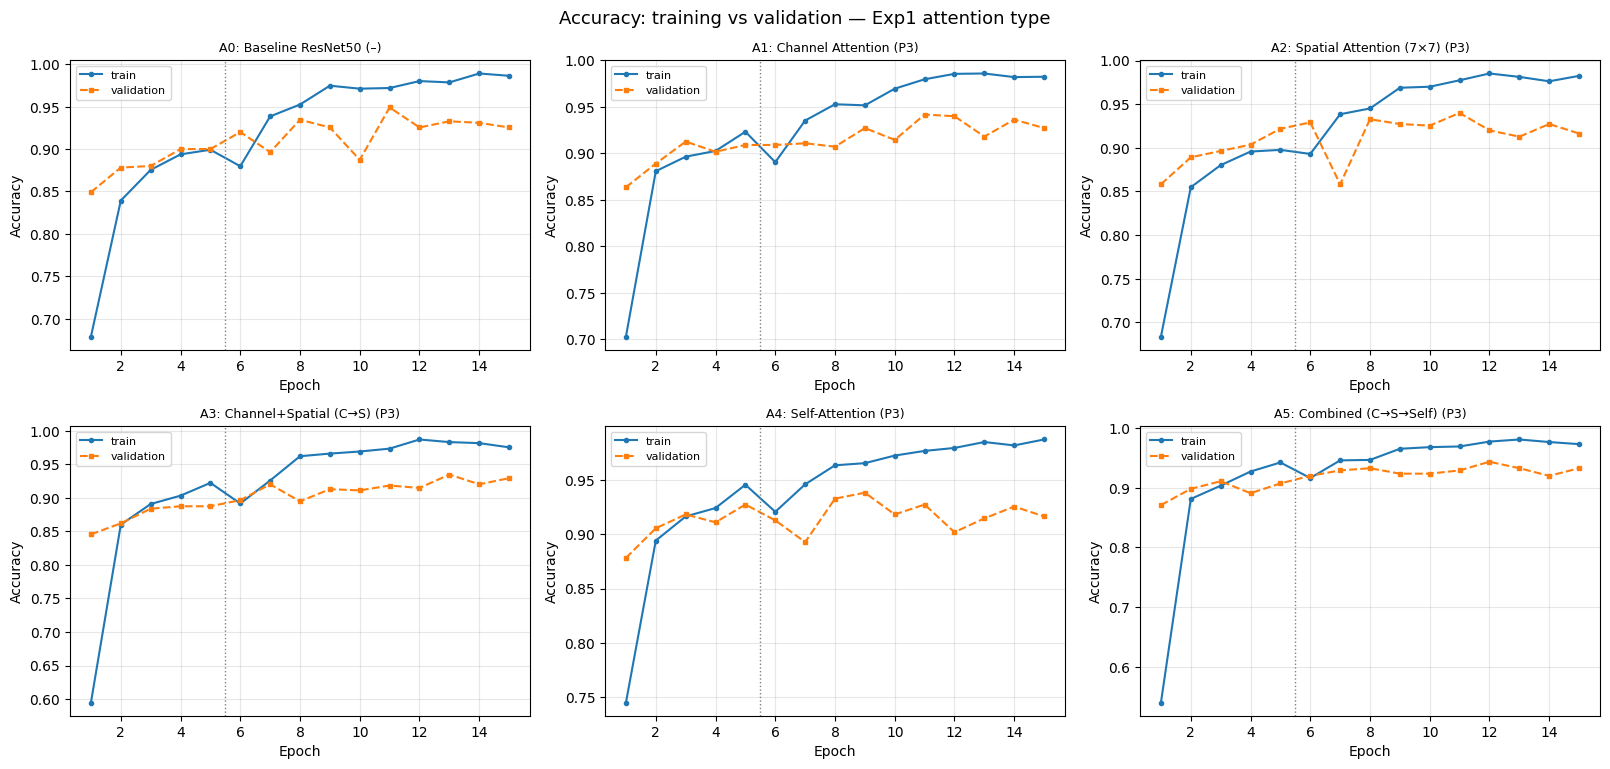
\includegraphics[width=0.98\textwidth]{plots/v_curves_accuracy_exp1.png}
\caption{Training and validation accuracy per epoch for A0--A5 (Experiment 1). Dotted line: start of fine-tuning (epoch 6).}
\end{figure}

\begin{figure}[H]
\centering
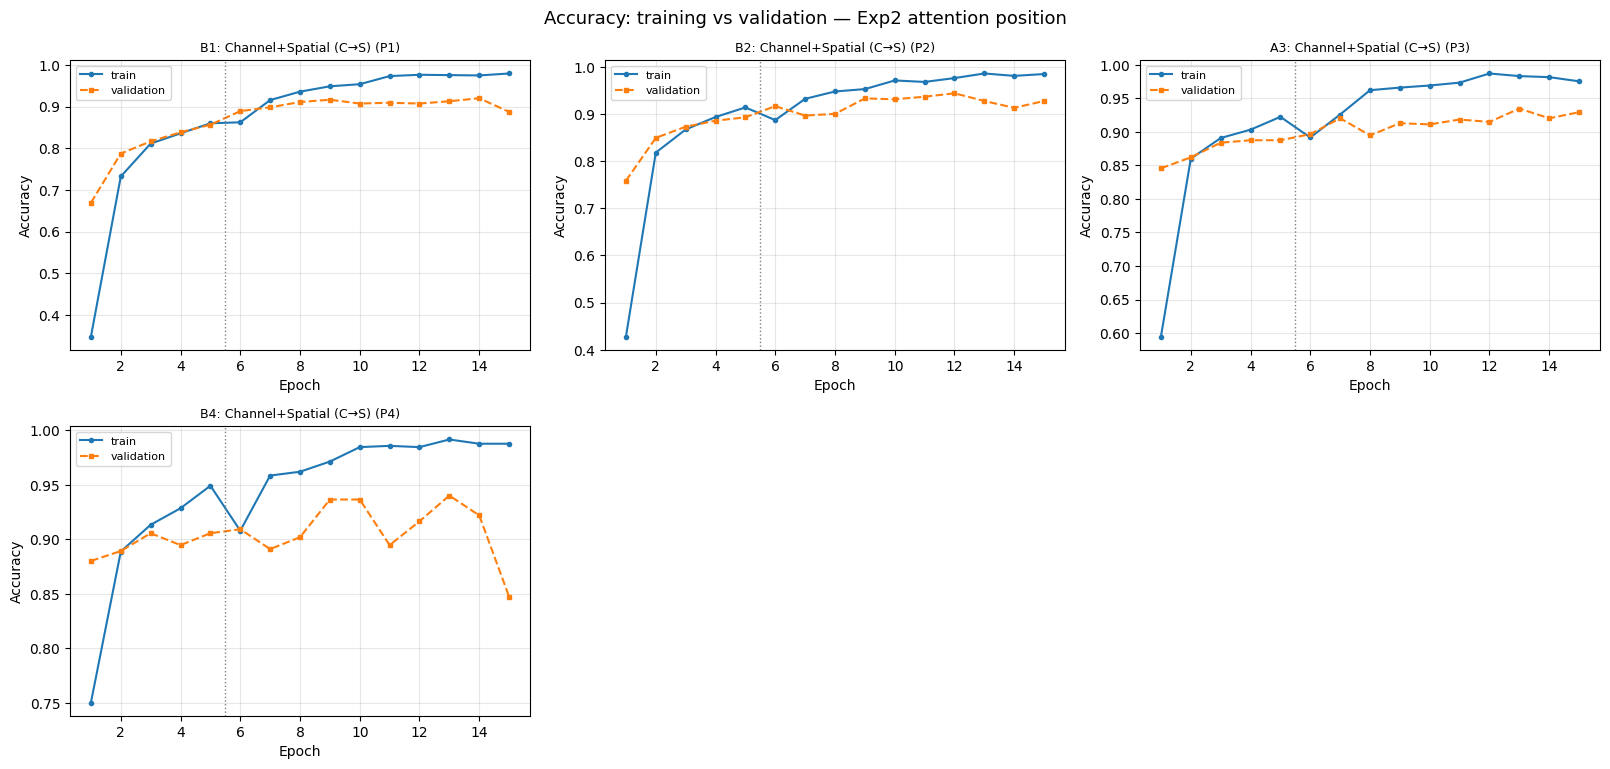
\includegraphics[width=0.98\textwidth]{plots/v_curves_accuracy_exp2.png}
\caption{Training and validation accuracy per epoch for B1--B4 (Experiment 2).}
\end{figure}

\textbf{Inference:} In all six models training accuracy rises quickly in the frozen-backbone stage, dips at epoch 6 when \texttt{conv5\_x} is unfrozen (for example the baseline falls from 0.8992 to 0.8797) and then
climbs to about 0.97--0.99, while validation accuracy plateaus at roughly 0.92--0.95, leaving a persistent train--validation gap (at the restored weights 0.037--0.066; baseline 0.047, channel 0.047, spatial 0.037,
channel+spatial 0.066, self-attention 0.049, combined 0.051). Validation accuracy is noisy for every model (the baseline fluctuates between 0.887 and 0.949, and spatial attention drops to 0.858 at epoch 7). Attention
therefore did not remove overfitting or make the learning smoother in a consistent way: only the self-attention models (A4, A5) show clearly smoother validation behaviour (validation-loss roughness 0.052 and 0.047 versus 0.087 for the baseline),
and the faster early convergence of self-attention, channel and combined attention (90\% validation accuracy at epochs 2, 3 and 3 versus 6) did not translate into a higher final accuracy than the baseline.

% ============================================================
\subsection*{25.2 Training and Validation Loss}
% ============================================================

Plot

\[
\text{Epoch}
\quad\text{versus}\quad
\mathcal{L}_{CE}.
\]

The graph should include training and validation loss.

Students should compare the convergence behavior of the baseline and
attention models.


\begin{figure}[H]
\centering
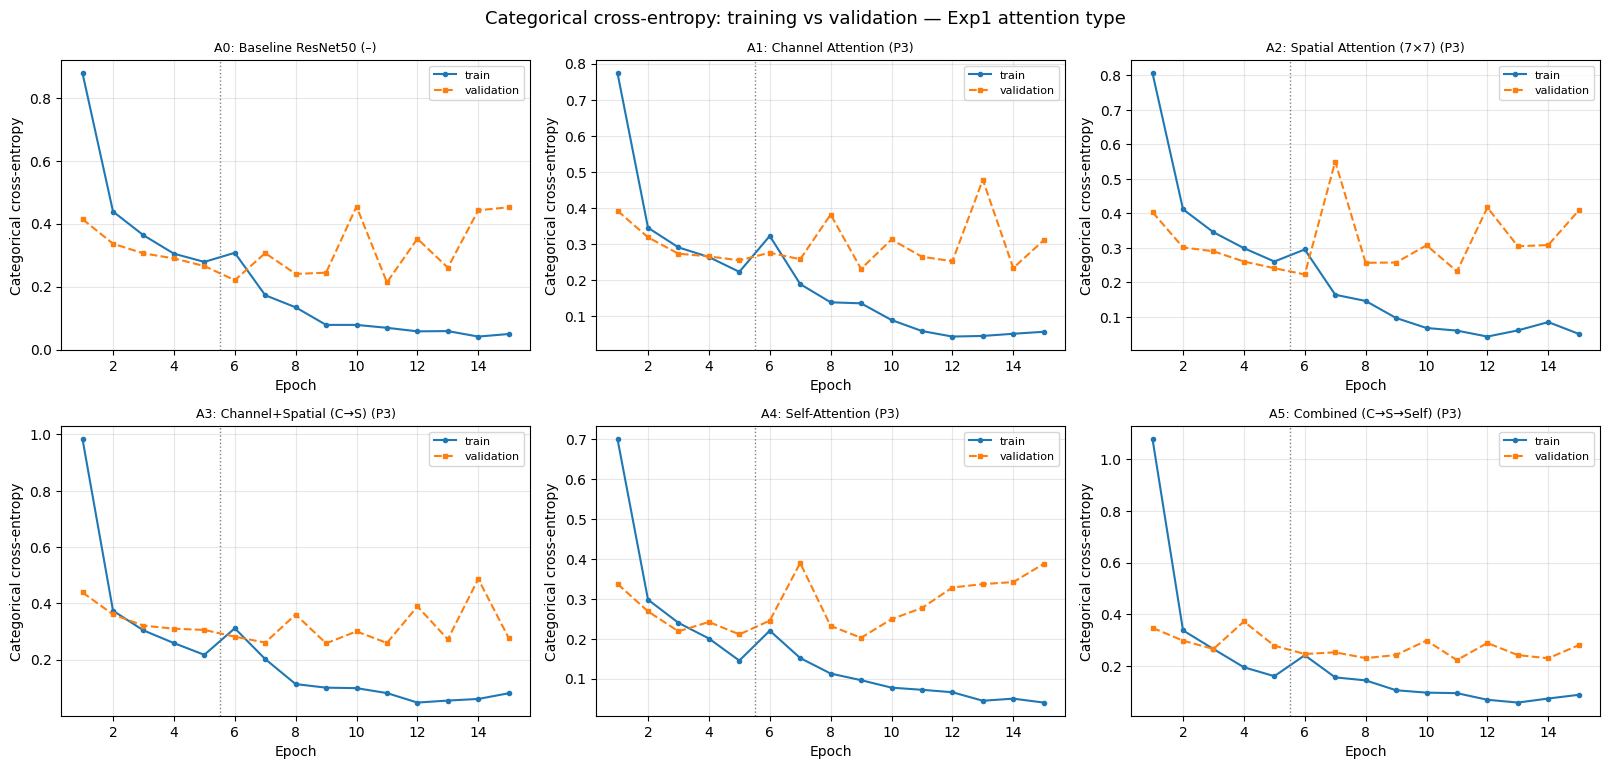
\includegraphics[width=0.98\textwidth]{plots/v_curves_loss_exp1.png}
\caption{Training and validation cross-entropy loss per epoch for A0--A5 (Experiment 1).}
\end{figure}

\begin{figure}[H]
\centering
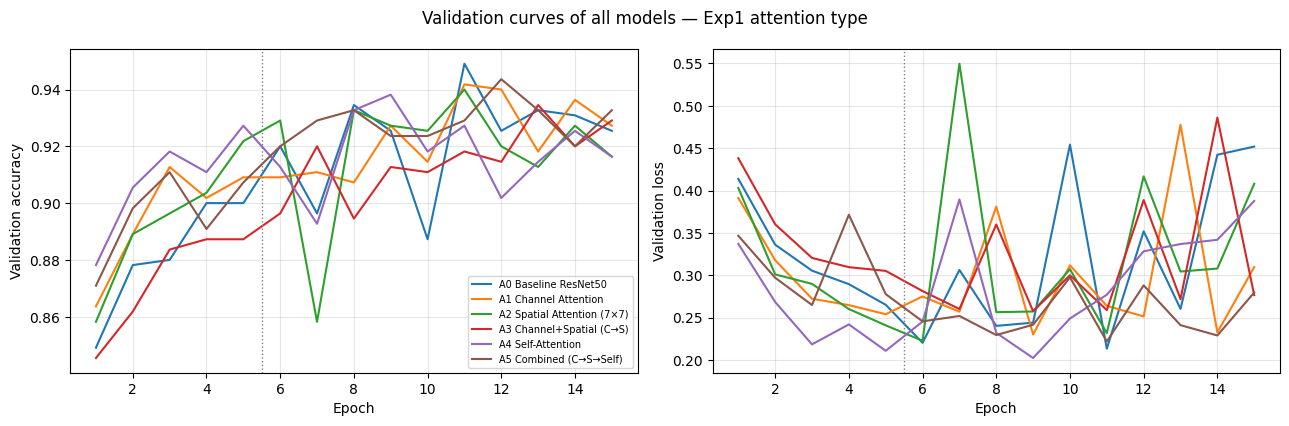
\includegraphics[width=0.95\textwidth]{plots/v_curves_val_overlay_exp1.png}
\caption{Validation accuracy and validation loss of A0--A5 overlaid (Experiment 1).}
\end{figure}

\textbf{Inference:} Training loss falls to about 0.04--0.09 by the end of fine-tuning for all models, whereas validation loss stays between about 0.2 and 0.5 and does not keep decreasing after epochs 6--9, which is the usual overfitting pattern.
The baseline's validation loss spikes at epochs 10 and 14--15 (about 0.45), spatial attention spikes to about 0.55 at epoch 7, and the self-attention model's validation loss rises steadily from about 0.20 at epoch 9 to about 0.39 at
epoch 15 while its training loss continues to fall (the epoch-9 weights were restored). The combined model has the flattest validation loss after epoch 6 (about 0.22--0.30). Overall the attention models converge in a similar number of epochs to the baseline and
show similar overfitting; the visible differences are in how smooth the validation loss is, not in a lower final value.

% ============================================================
\subsection*{25.3 Attention Mechanism versus Accuracy}
% ============================================================

Generate a bar graph:

\[
x=
\text{Attention Mechanism}
\]

and

\[
y=
\text{Classification Accuracy}.
\]

Possible entries are:

\begin{center}

Baseline,
Channel,
Spatial,
Channel+Spatial,
Self-Attention,
SE,
ECA,
CBAM.

\end{center}


\begin{figure}[H]
\centering
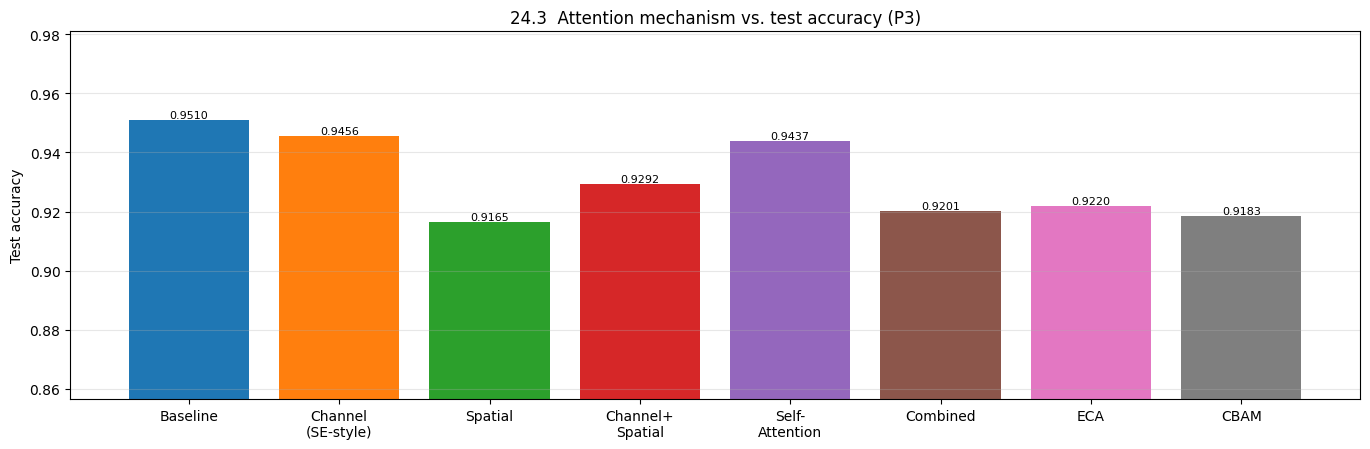
\includegraphics[width=0.95\textwidth]{plots/v_bar_mech_accuracy.png}
\caption{Test accuracy of the baseline and of the attention mechanisms at $P_3$.}
\end{figure}

\begin{figure}[H]
\centering
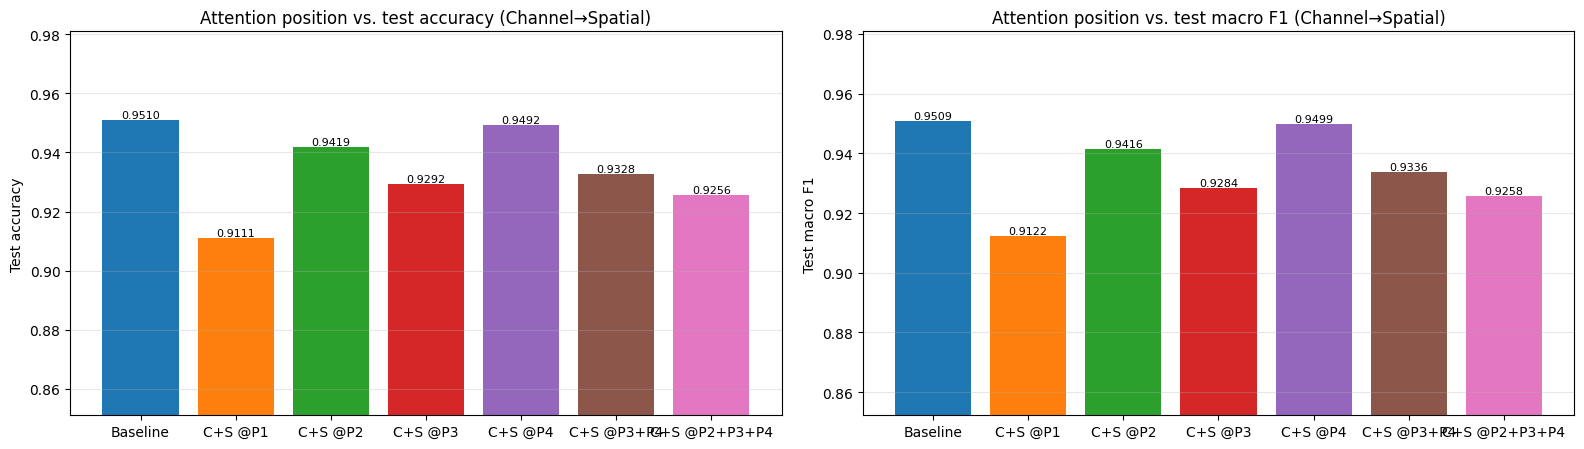
\includegraphics[width=0.98\textwidth]{plots/v_bar_position.png}
\caption{Test accuracy and macro F1 versus attention position (Channel$\rightarrow$Spatial; single-, multi-position and baseline).}
\end{figure}

\textbf{Inference:} The baseline (0.9510) is the tallest bar, followed by channel (0.9456), self-attention (0.9437), channel+spatial (0.9292), ECA (0.9220), combined (0.9201), CBAM (0.9183) and spatial (0.9165). The y-axis of the plot starts at about 0.86, which visually exaggerates
differences of a few percentage points. The position chart shows that attention at $P_4$ (0.9492) and $P_2$ (0.9419) is closer to the baseline than at $P_3$ (0.9292) or $P_1$ (0.9111), and that the multi-position models ($P_3+P_4$: 0.9328, $P_2+P_3+P_4$: 0.9256) are not better than $P_4$ alone.

% ============================================================
\subsection*{25.4 Attention Mechanism versus Macro F1}
% ============================================================

Similarly, plot:

\[
x=
\text{Attention Mechanism}
\]

and

\[
y=
\text{Macro F1-score}.
\]

This comparison is useful when the class-wise performance is not uniform.


\begin{figure}[H]
\centering
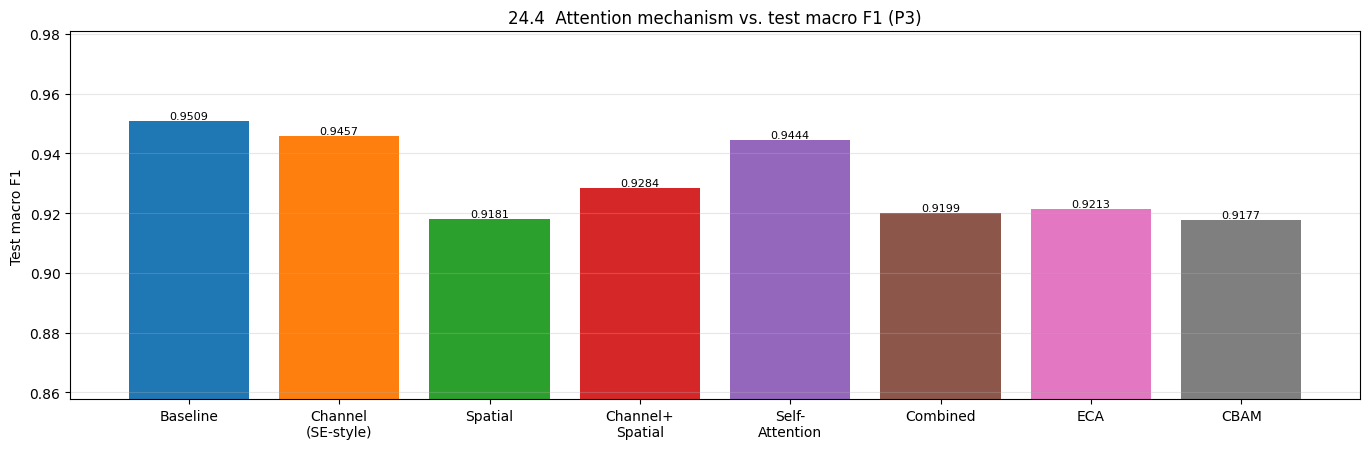
\includegraphics[width=0.95\textwidth]{plots/v_bar_mech_f1.png}
\caption{Macro F1 of the baseline and of the attention mechanisms at $P_3$.}
\end{figure}

\textbf{Inference:} The macro-F1 ordering matches the accuracy ordering except that spatial attention (0.9181) is now slightly above CBAM (0.9177): baseline 0.9509, channel 0.9457, self-attention 0.9444, channel+spatial 0.9284, ECA 0.9213, combined 0.9199, spatial 0.9181, CBAM 0.9177.
Accuracy and macro F1 differ by at most 0.002 for every model (for example 0.9510 versus 0.9509 for the baseline), so the five classes are classified with similar balance of precision and recall and the F1 view leads to the same conclusion as the accuracy view.

% ============================================================
\subsection*{25.5 Accuracy versus Model Parameters}
% ============================================================

Create a scatter plot using:

\[
x=
\text{Total Model Parameters}
\]

and

\[
y=
\text{Test Accuracy}.
\]

Each point should represent one attention mechanism.

This allows the student to study the

\[
\boxed{
\text{Accuracy--Complexity Trade-off}
}
\]

instead of evaluating accuracy independently.


\begin{figure}[H]
\centering
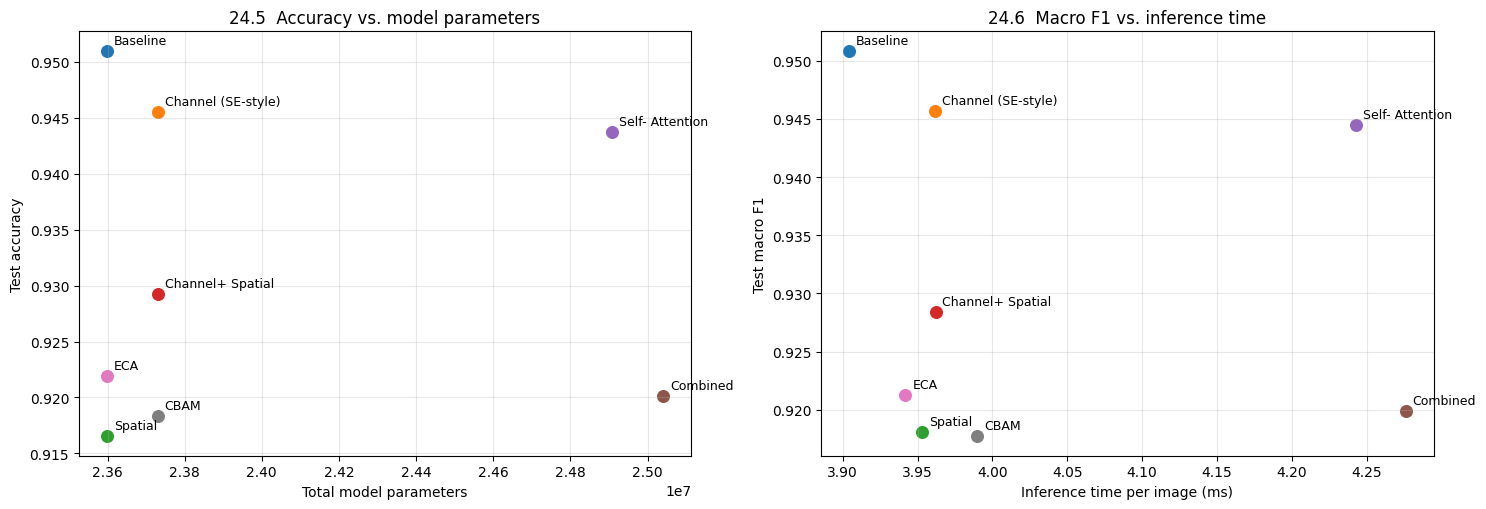
\includegraphics[width=0.98\textwidth]{plots/v_scatter_tradeoffs.png}
\caption{Left: test accuracy versus total parameters; right: macro F1 versus inference time per image (one point per mechanism at $P_3$).}
\end{figure}

\textbf{Inference:} The points show no positive relation between parameters and accuracy. The baseline (23.60M parameters) has the highest accuracy; ECA and spatial attention add almost nothing (23.60M) but are lower (0.9220, 0.9165); the SE-style channel and channel+spatial/CBAM modules
cluster at 23.73M with accuracies between 0.9183 and 0.9456; self-attention (24.91M) and the combined model (25.04M) are the most expensive and reach 0.9437 and 0.9201. The accuracy--complexity trade-off is therefore unfavourable for every attention
module in this experiment: none of them moves up from the baseline as parameters increase.

% ============================================================
\subsection*{25.6 Macro F1 versus Inference Time}
% ============================================================

Plot:

\[
x=
\text{Inference Time per Image}
\]

and

\[
y=
\text{Macro F1-score}.
\]

Students should analyze whether additional computational cost produces a
meaningful increase in classification performance.


\textbf{Inference:} The baseline is both the fastest model (3.904 ms/img) and the one with the highest macro F1 (0.9509). The lightweight modules (ECA, spatial, SE, CBAM) lie between 3.94 and 3.99 ms with macro F1 between 0.9177 and 0.9457, while the two self-attention-based models are the slowest
(4.243 and 4.276 ms) with F1 0.9444 and 0.9199. No point reaches a higher F1 than the baseline at any additional inference cost, so the extra computation did not give a meaningful increase in classification performance here (for example self-attention: $+0.339$ ms, $+8.7\%$, for a 0.0065 lower F1).

% ============================================================
\section*{26. Confusion Matrix Analysis}
% ============================================================

Generate a confusion matrix for:

\begin{enumerate}

\item baseline ResNet50; and

\item the selected attention-based ResNet50.

\end{enumerate}

The confusion matrix should contain all five flower classes.

Students should analyze:

\begin{itemize}

\item which classes are most accurately classified;

\item which classes are frequently confused;

\item which class benefits most from attention;

\item whether attention reduces a particular type of confusion; and

\item whether the improved overall accuracy is distributed across classes.

\end{itemize}


The selected attention model is the model among A1--A5 (attention at $P_3$) with the highest \emph{validation} accuracy (A1 0.9273, A2 0.9291, A3 0.9127, \textbf{A4 0.9382}, A5 0.9291); it is therefore
\textbf{A4: Self-Attention at $P_3$}. (On the test set the SE-style channel model A1 is more accurate than A4; the selection used the validation set only.)

\begin{figure}[H]
\centering
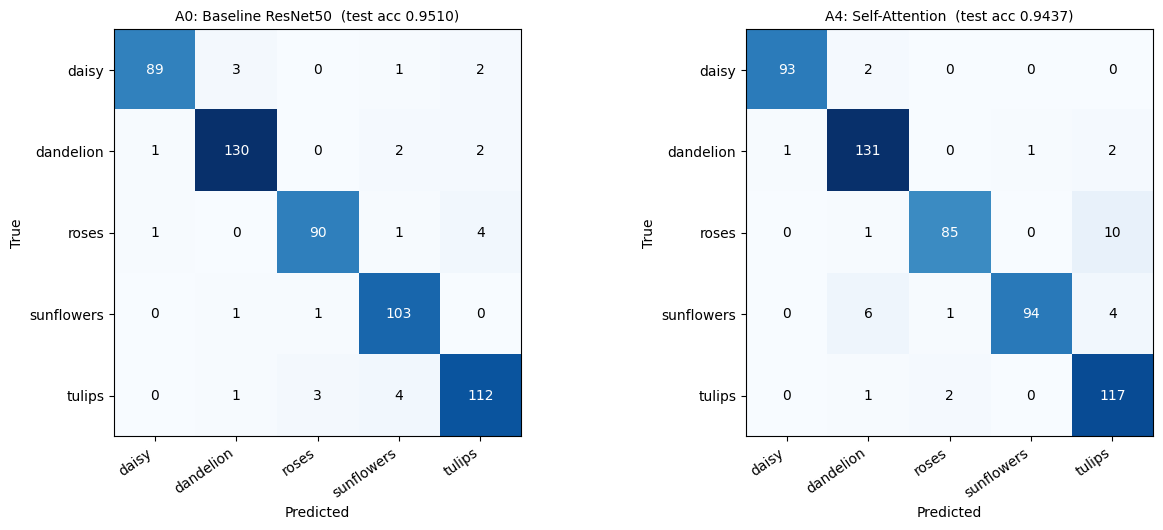
\includegraphics[width=0.95\textwidth]{plots/v_confusion_matrices.png}
\caption{Confusion matrices on the test set: baseline ResNet50 (left, accuracy 0.9510) and the selected self-attention model A4 (right, accuracy 0.9437).}
\end{figure}

\textbf{Baseline (A0)} --- rows: true class, columns: predicted class.

\begin{center}
\begin{tabular}{|l|c|c|c|c|c|}
\hline
\textbf{True $\backslash$ Pred.} & \textbf{daisy} & \textbf{dandelion} & \textbf{roses} & \textbf{sunflowers} & \textbf{tulips} \\
\hline
daisy & 89 & 3 & 0 & 1 & 2 \\
\hline
dandelion & 1 & 130 & 0 & 2 & 2 \\
\hline
roses & 1 & 0 & 90 & 1 & 4 \\
\hline
sunflowers & 0 & 1 & 1 & 103 & 0 \\
\hline
tulips & 0 & 1 & 3 & 4 & 112 \\
\hline
\end{tabular}
\end{center}

\textbf{Self-attention (A4)}

\begin{center}
\begin{tabular}{|l|c|c|c|c|c|}
\hline
\textbf{True $\backslash$ Pred.} & \textbf{daisy} & \textbf{dandelion} & \textbf{roses} & \textbf{sunflowers} & \textbf{tulips} \\
\hline
daisy & 93 & 2 & 0 & 0 & 0 \\
\hline
dandelion & 1 & 131 & 0 & 1 & 2 \\
\hline
roses & 0 & 1 & 85 & 0 & 10 \\
\hline
sunflowers & 0 & 6 & 1 & 94 & 4 \\
\hline
tulips & 0 & 1 & 2 & 0 & 117 \\
\hline
\end{tabular}
\end{center}

\textbf{Per-class test metrics.}

\begin{center}
\resizebox{\textwidth}{!}{
\begin{tabular}{|l|c|c|c|c|c|c|c|c|c|c|}
\hline
\textbf{Class} & \textbf{Support} & \textbf{P (A0)} & \textbf{R (A0)} & \textbf{F1 (A0)} & \textbf{P (A4)} & \textbf{R (A4)} & \textbf{F1 (A4)} & \textbf{$\Delta$P} & \textbf{$\Delta$R} & \textbf{$\Delta$F1} \\
\hline
daisy & 95 & 0.9780 & 0.9368 & 0.9570 & 0.9894 & 0.9789 & 0.9841 & +0.0114 & +0.0421 & +0.0271 \\
\hline
dandelion & 135 & 0.9630 & 0.9630 & 0.9630 & 0.9291 & 0.9704 & 0.9493 & -0.0339 & +0.0074 & -0.0137 \\
\hline
roses & 96 & 0.9574 & 0.9375 & 0.9474 & 0.9659 & 0.8854 & 0.9239 & +0.0085 & -0.0521 & -0.0235 \\
\hline
sunflowers & 105 & 0.9279 & 0.9810 & 0.9537 & 0.9895 & 0.8952 & 0.9400 & +0.0616 & -0.0858 & -0.0137 \\
\hline
tulips & 120 & 0.9333 & 0.9333 & 0.9333 & 0.8797 & 0.9750 & 0.9249 & -0.0536 & +0.0417 & -0.0084 \\
\hline
\end{tabular}}
\end{center}

\textbf{Inference:} \textbf{Most accurately classified:} for the baseline the highest recall is for sunflowers (0.9810, 103 of 105) and dandelion (0.9630, F1 0.9630); for A4 the highest recall is for daisy (0.9789) and tulips (0.9750).
\textbf{Frequent confusions:} the baseline's most frequent errors are tulips$\rightarrow$sunflowers (4), roses$\rightarrow$tulips (4), tulips$\rightarrow$roses (3) and daisy$\rightarrow$dandelion (3); for A4 they are
roses$\rightarrow$tulips (10), sunflowers$\rightarrow$dandelion (6), sunflowers$\rightarrow$tulips (4), tulips$\rightarrow$roses (2) and dandelion$\rightarrow$tulips (2).
\textbf{Which class benefits:} daisy benefits most (F1 0.9570 $\rightarrow$ 0.9841; recall +4.2 points, 89 $\rightarrow$ 93 correct) and the tulips recall also rises (+4.2 points, 112 $\rightarrow$ 117) although its precision falls by 5.4 points because
more roses and sunflowers are predicted as tulips (roses$\rightarrow$tulips 4 $\rightarrow$ 10, sunflowers$\rightarrow$tulips 0 $\rightarrow$ 4). The confusion tulips$\rightarrow$sunflowers disappears (4 $\rightarrow$ 0) but sunflowers$\rightarrow$dandelion increases (1 $\rightarrow$ 6).
\textbf{Distribution of the change:} the overall accuracy is 0.73 points lower (520 versus 524 correct) and this hides large class-specific shifts: the recall of roses falls by 5.2 points and that of sunflowers by 8.6 points, whereas daisy and tulips improve.
Attention therefore reduced one type of confusion (tulips$\rightarrow$sunflowers) but created others, and the accuracy change is not evenly distributed across classes.

% ============================================================
\section*{27. Qualitative Analysis of Attention}
% ============================================================

Quantitative classification performance does not directly explain where the
network obtains evidence for its prediction.

Students must therefore perform qualitative analysis.

The visual analysis should include:

\begin{itemize}

\item internal attention maps;

\item attention overlays;

\item intermediate feature maps; and

\item Grad-CAM explanations.

\end{itemize}

Students should preferably use the same input image when comparing different
models.

% ============================================================
\section*{28. Grad-CAM Visualization}
% ============================================================

Gradient-weighted Class Activation Mapping (Grad-CAM) provides a
class-specific visualization of the regions contributing to a prediction.

Let

\[
A^k
\]

represent feature map $k$ from a selected convolutional layer.

For class score $y^c$, the importance coefficient is:

\[
\alpha_k^c
=
\frac{1}{HW}
\sum_i
\sum_j
\frac{\partial y^c}
{\partial A_{ij}^k}.
\]

The Grad-CAM map is:

\[
L_{\mathrm{Grad-CAM}}^c
=
\operatorname{ReLU}
\left(
\sum_k
\alpha_k^c A^k
\right).
\]

The map should be resized to the original image resolution and overlaid on
the input.

Students should compare:

\[
\boxed{
\text{Input}
\;|\;
\text{Baseline Grad-CAM}
\;|\;
\text{Attention Model Grad-CAM}
}
\]

for the same image.


Grad-CAM was computed for the \emph{predicted} class on the final $7\times7\times2048$ feature map entering global average pooling (class score = logit; ReLU, then division by the maximum).
The representative images are the first test image of each class (test indices: daisy 1, dandelion 9, roses 0, sunflowers 5, tulips 3); all five were classified correctly by A0, A1, A3 and A4.

\begin{figure}[H]
\centering
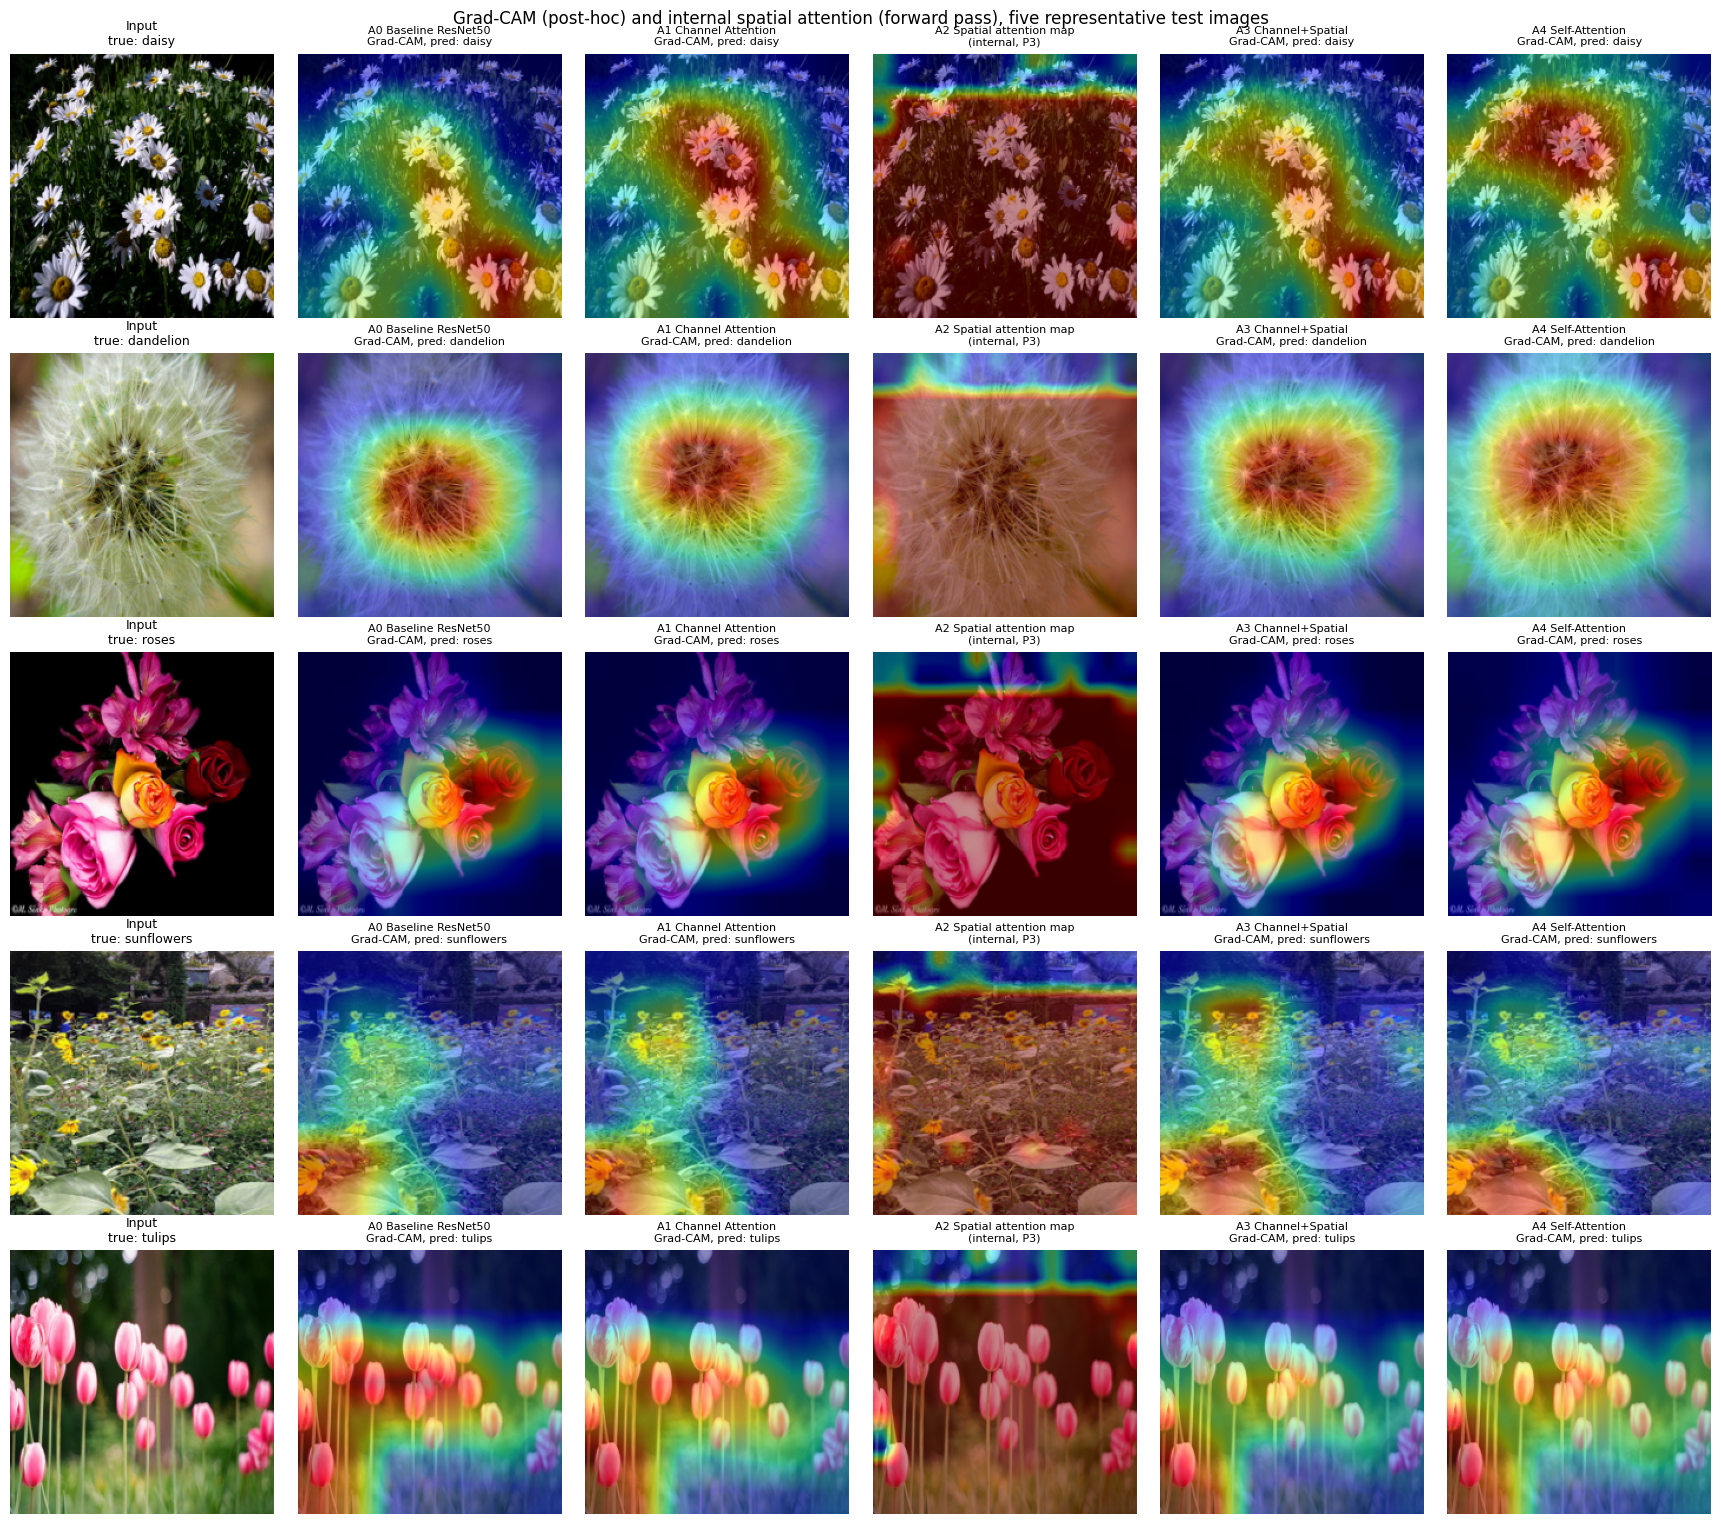
\includegraphics[width=0.98\textwidth]{plots/v_gradcam_layout.png}
\caption{Grad-CAM (post-hoc) for the baseline (A0), channel attention (A1), channel+spatial (A3) and self-attention (A4), together with the internal spatial attention map of A2, for five representative test images.}
\end{figure}

\begin{center}
\resizebox{\textwidth}{!}{
\begin{tabular}{|l|c|c|c|c|c|c|c|c|}
\hline
\textbf{Image} & \textbf{Cov. A0} & \textbf{Ent. A0} & \textbf{Cov. A1} & \textbf{Ent. A1} & \textbf{Cov. A3} & \textbf{Ent. A3} & \textbf{Cov. A4} & \textbf{Ent. A4} \\
\hline
daisy & 0.3391 & 0.9336 & 0.4769 & 0.9578 & 0.4334 & 0.9539 & 0.5026 & 0.9689 \\
\hline
dandelion & 0.2354 & 0.8961 & 0.2775 & 0.9154 & 0.2779 & 0.9167 & 0.3935 & 0.9571 \\
\hline
roses & 0.1448 & 0.8324 & 0.1581 & 0.8258 & 0.1882 & 0.8362 & 0.2180 & 0.8999 \\
\hline
sunflowers & 0.1152 & 0.8699 & 0.1746 & 0.8245 & 0.2502 & 0.9063 & 0.1510 & 0.8461 \\
\hline
tulips & 0.4006 & 0.8927 & 0.3416 & 0.8932 & 0.2360 & 0.8862 & 0.3321 & 0.9038 \\
\hline
\end{tabular}}
\end{center}

Whole-test-set means: coverage (fraction of the map $\ge0.5$) A0 0.2354, A1 0.2099, A2 0.1798, A3 0.2028, A4 0.2738, A5 0.3065; normalised entropy 0.8422, 0.8265, 0.8175, 0.8244, 0.8876, 0.9014.

\textbf{Inference:} On these five images the Grad-CAM maps of the attention models are broadly similar to the baseline's: all models highlight the same dominant regions (the dandelion head, the orange and red roses at the centre-right of the roses image, the lower band of tulip heads).
The differences are in extent rather than location. For the daisy image the baseline concentrates on flowers in the lower right whereas the channel, channel+spatial and self-attention models cover a larger area that also includes the upper-left flowers (coverage 0.339 $\rightarrow$ 0.477, 0.433, 0.503);
for the dandelion the self-attention map has a larger high-activation region (coverage 0.394 versus 0.235); for the tulips the attention models move part of the activation from the lower band to the upper-left tulip heads and coverage decreases (0.401 $\rightarrow$ 0.342, 0.236, 0.332); for the sunflowers
image the activation is spread over a wide part of the field for all models. Averaged over the test set, channel, spatial and channel+spatial attention give more compact Grad-CAM maps than the baseline whereas self-attention gives broader ones.
The visible evidence therefore does not show that attention consistently suppresses background or sharpens the focus on the flower.

% ============================================================
\subsection*{28.1 Grad-CAM Interpretation}
% ============================================================

Students should qualitatively determine whether the attention model:

\begin{itemize}

\item focuses more strongly on the flower;

\item suppresses irrelevant background regions;

\item concentrates on petals;

\item concentrates on the central flower structure;

\item attends to discriminative edges;

\item distributes activation across the entire flower;

\item incorrectly focuses on leaves;

\item incorrectly focuses on background objects; or

\item changes its focus for an incorrect prediction.

\end{itemize}

Students should avoid unsupported statements such as:

\begin{quote}
``The Grad-CAM of Model A is better.''
\end{quote}

Instead, the observation should describe visible evidence.

For example:

\begin{quote}
The baseline network activates both the flower and surrounding leaves,
whereas the attention-based model produces stronger activation over the petal
region and weaker activation over the background.
\end{quote}


\textbf{Observations (based on the images and statistics above).}

\begin{itemize}
\item \textbf{Focus on the flower:} in the dandelion and roses images every model concentrates its strongest activation on the flower head or the central flower cluster.
\item \textbf{Background suppression:} no clear suppression is visible; in the daisy and sunflowers field images the activation extends over large parts of the scene for all models, and the self-attention and combined models have the largest coverage (0.2738 and 0.3065 versus 0.2354 for the baseline).
\item \textbf{Compactness:} channel (0.2099), spatial (0.1798), channel+spatial (0.2028), ECA (0.1919) and CBAM (0.1816) give slightly smaller above-threshold regions than the baseline.
\item \textbf{Incorrect predictions:} over the whole test set the Grad-CAM maps of misclassified images are \emph{more} concentrated than those of correctly classified images for every model (coverage 0.147 versus 0.240 for the baseline and 0.157 versus 0.281 for A4; entropy 0.789 versus 0.845 and 0.837 versus 0.891), see Section 31.
\end{itemize}

% ============================================================
\section*{29. Internal Attention Maps}
% ============================================================

An important objective of this experiment is to distinguish between:

\[
\boxed{\text{Internal Attention}}
\]

and

\[
\boxed{\text{Post-hoc Explanation}}
\]

because they are not the same.

An attention module directly computes weights during the forward pass.

Grad-CAM, in contrast, is generated after prediction using gradients.

% ============================================================
\subsection*{29.1 Channel-Attention Visualization}
% ============================================================

For channel attention:

\[
M_c(F)
=
[m_1,m_2,\ldots,m_C].
\]

Students should visualize the learned channel importance values using a bar
graph.

Instead of displaying every channel when $C$ is large, the student may show
the top-$K$ channels.

Recommended values are:

\[
K=10
\]

or

\[
K=20.
\]

Students should comment on whether:

\begin{itemize}

\item a small number of channels receive strong weights;

\item many channels contribute similarly; or

\item channel weighting changes substantially for different input images.

\end{itemize}


\begin{figure}[H]
\centering
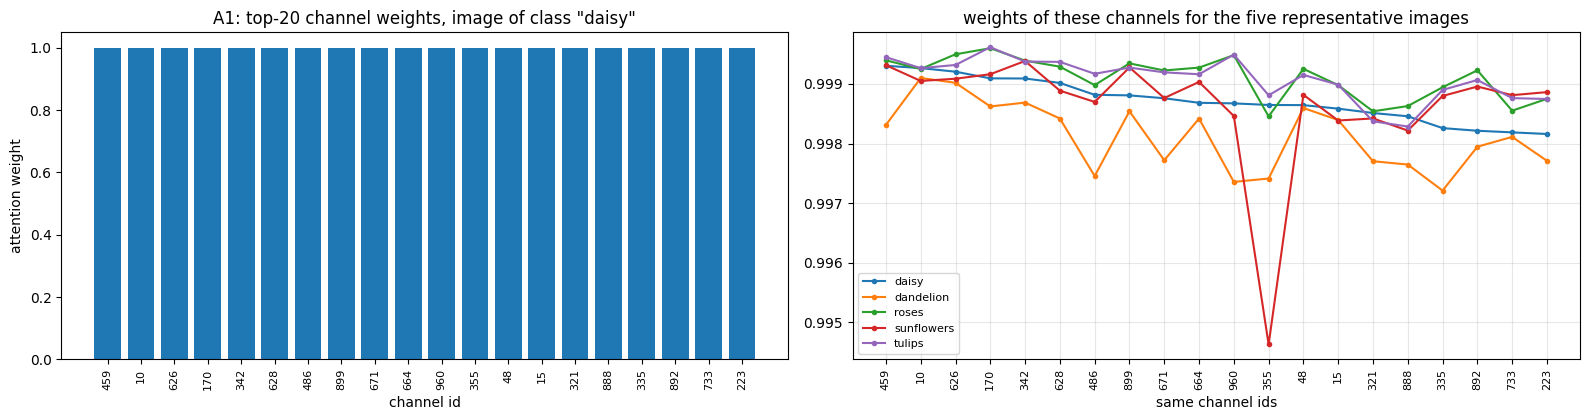
\includegraphics[width=0.98\textwidth]{plots/v_channel_weights_A1.png}
\caption{Channel attention of A1 at $P_3$: top-20 channel weights for a daisy image (left) and the weights of the same channels for the five representative images (right).}
\end{figure}

\begin{figure}[H]
\centering
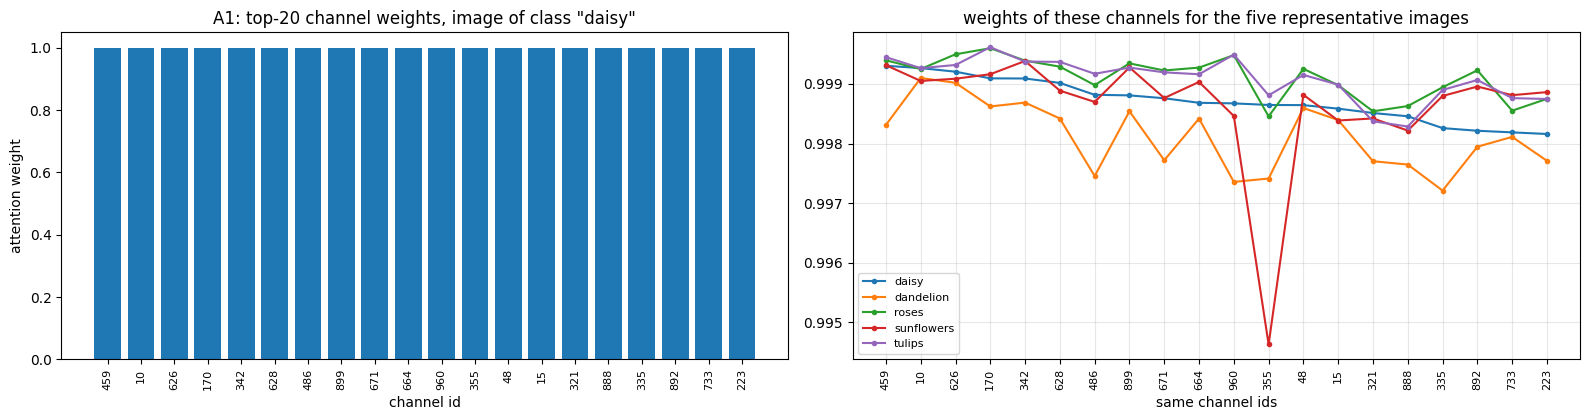
\includegraphics[width=0.98\textwidth]{plots/v_channel_weights_A3.png}
\caption{Channel attention of A3 (channel$\rightarrow$spatial) at $P_3$: top-20 channel weights and the weights of the same channels for the five representative images.}
\end{figure}

\begin{center}
\resizebox{\textwidth}{!}{
\begin{tabular}{|l|c|c|c|c|c|c|}
\hline
\textbf{Image (A1)} & \textbf{Mean weight} & \textbf{Std over channels} & \textbf{Min} & \textbf{Max} & \textbf{\# channels $>0.5$} & \textbf{Top-10 share} \\
\hline
daisy & 0.5895 & 0.4267 & 0.0018 & 0.9993 & 603 & 0.0166 \\
\hline
dandelion & 0.5885 & 0.4227 & 0.0020 & 0.9991 & 600 & 0.0166 \\
\hline
roses & 0.5917 & 0.4334 & 0.0014 & 0.9996 & 608 & 0.0165 \\
\hline
sunflowers & 0.5880 & 0.4291 & 0.0020 & 0.9994 & 600 & 0.0166 \\
\hline
tulips & 0.5911 & 0.4324 & 0.0015 & 0.9996 & 610 & 0.0165 \\
\hline
\end{tabular}}
\end{center}

\begin{center}
\resizebox{\textwidth}{!}{
\begin{tabular}{|l|c|c|c|c|c|c|}
\hline
\textbf{Image (A3)} & \textbf{Mean weight} & \textbf{Std over channels} & \textbf{Min} & \textbf{Max} & \textbf{\# channels $>0.5$} & \textbf{Top-10 share} \\
\hline
daisy & 0.6141 & 0.4071 & 0.0009 & 0.9994 & 636 & 0.0159 \\
\hline
dandelion & 0.6084 & 0.3896 & 0.0038 & 0.9981 & 636 & 0.0160 \\
\hline
roses & 0.6152 & 0.4138 & 0.0006 & 0.9995 & 638 & 0.0159 \\
\hline
sunflowers & 0.6148 & 0.4078 & 0.0013 & 0.9991 & 636 & 0.0159 \\
\hline
tulips & 0.6170 & 0.4177 & 0.0003 & 0.9998 & 640 & 0.0158 \\
\hline
\end{tabular}}
\end{center}

Whole-test-set statistics: A1 --- standard deviation over channels (average per image) 0.4272, standard deviation over images (average per channel) 0.0170, mean pairwise correlation of the weight vectors of different images 0.9966; A3 --- 0.4050, 0.0253 and 0.9934.

\textbf{Inference:} Many channels contribute strongly and almost equally rather than a small number dominating: the 20 highest weights are all about 0.998--0.9996 (saturated at 1), roughly 600 of the 1024 channels (A1) or 636--640 (A3) have weights above 0.5, and the weights are bimodal (mean about 0.59--0.62 with a standard deviation of about 0.4,
minimum near 0.001, maximum near 1.0). The top-10 channels hold only about 1.6--1.7\% of the total weight. The channel weighting is also almost the same for every image: the weight vectors of different images have a correlation of 0.9966 (A1) and 0.9934 (A3), and the
standard deviation of a channel's weight over images is only 0.017--0.025; differences between the five representative images appear only in the third or fourth decimal (for example the sunflowers image dips to about 0.9946 at one channel while the others stay above 0.997). At $P_3$ the channel module therefore acts mainly as a nearly fixed, input-independent
selection of channels rather than as an image-specific attention.

% ============================================================
\subsection*{29.2 Spatial-Attention Visualization}
% ============================================================

For spatial attention:

\[
M_s(F)
\in
\mathbb{R}^{H\times W}.
\]

Resize the attention map to:

\[
224\times224
\]

and overlay it on the input image.

Display:

\[
\boxed{
\text{Input}
\;|\;
\text{Spatial Attention Map}
\;|\;
\text{Attention Overlay}
}
\]

Students should identify the image regions receiving high attention values.


\begin{figure}[H]
\centering
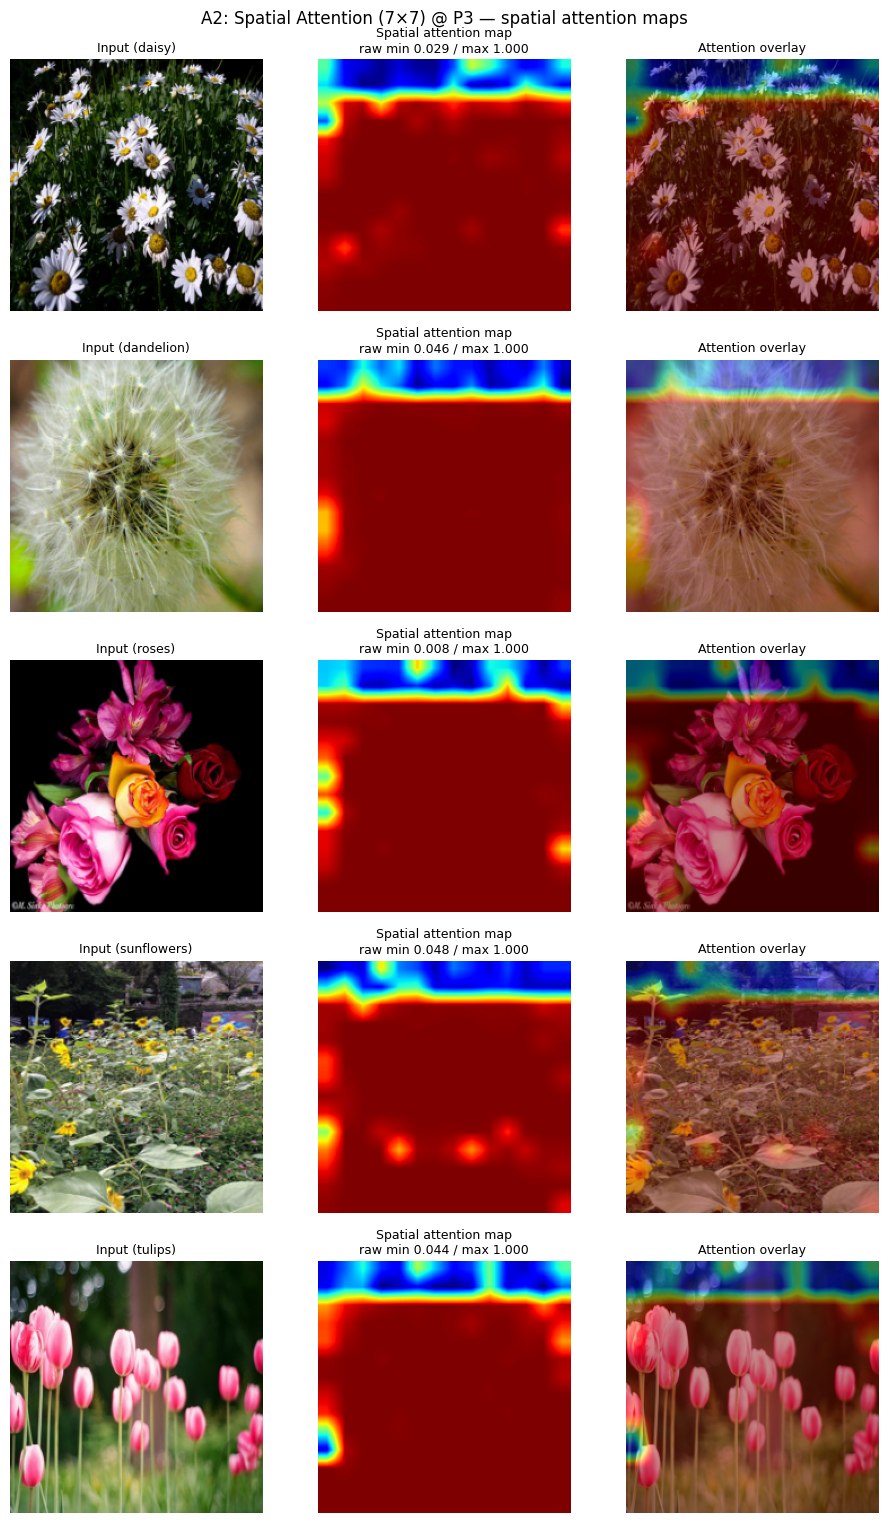
\includegraphics[width=0.70\textwidth]{plots/v_spatial_maps_A2.png}
\caption{Spatial attention of A2 (spatial only, $7\times7$ kernel) at $P_3$: input, attention map (min--max normalised for display) and overlay for the five representative images.}
\end{figure}

\begin{figure}[H]
\centering
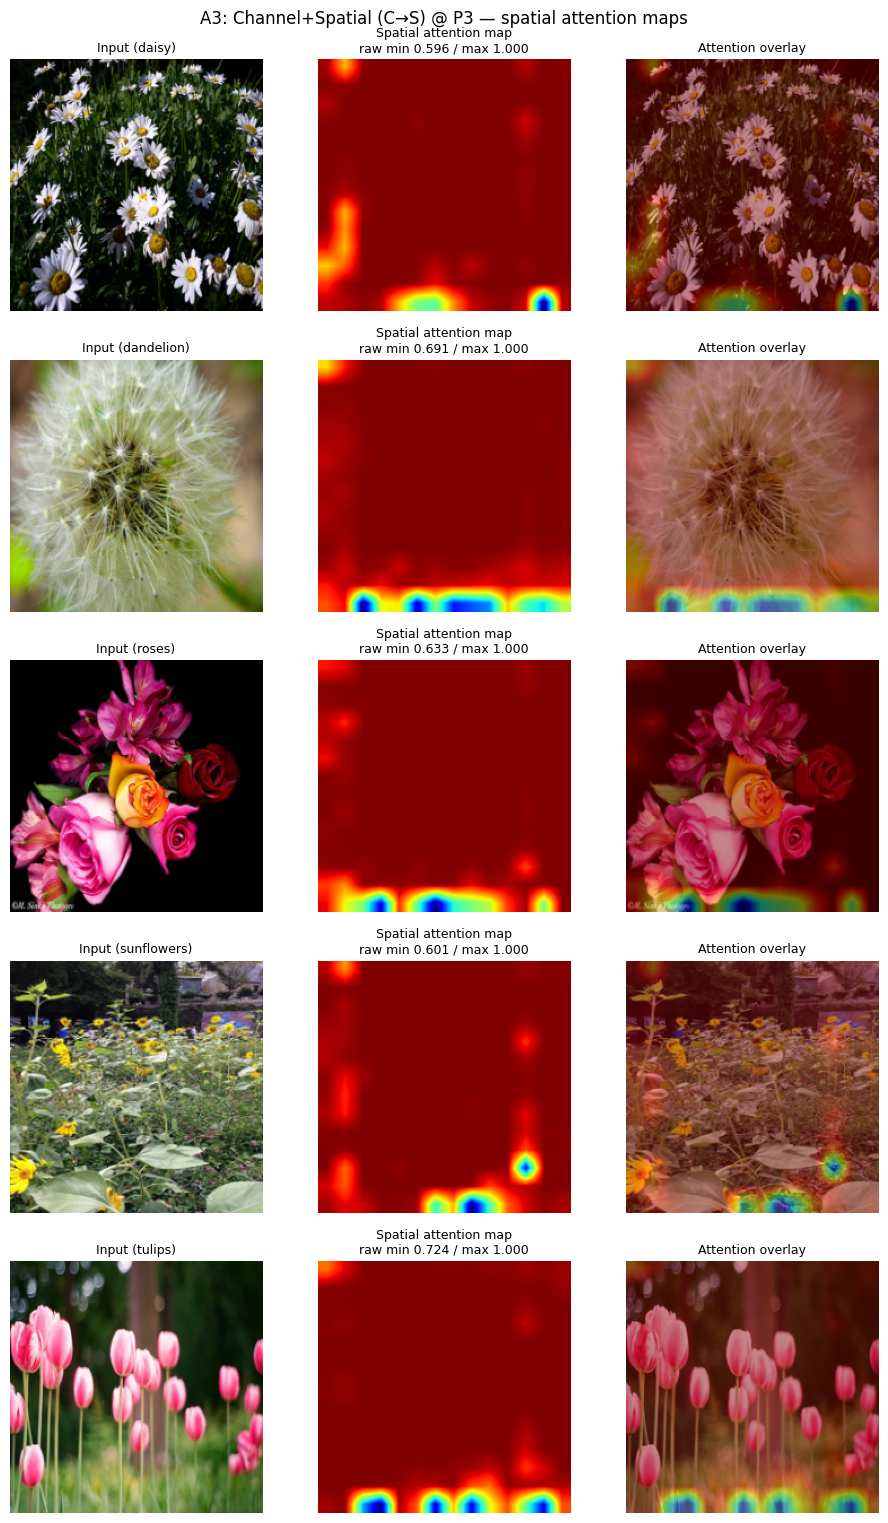
\includegraphics[width=0.70\textwidth]{plots/v_spatial_maps_A3.png}
\caption{Spatial attention of A3 (channel$\rightarrow$spatial) at $P_3$: input, attention map and overlay.}
\end{figure}

\begin{center}
\begin{tabular}{|l|c|c|c|c|c|c|}
\hline
\textbf{Model} & \textbf{daisy} & \textbf{dandelion} & \textbf{roses} & \textbf{sunflowers} & \textbf{tulips} & \textbf{Mean (test set)} \\
\hline
A2: raw minimum of map & 0.029 & 0.046 & 0.008 & 0.048 & 0.044 & 0.885 \\
\hline
A3: raw minimum of map & 0.596 & 0.691 & 0.633 & 0.601 & 0.724 & 0.986 \\
\hline
\end{tabular}
\end{center}

\textbf{Inference:} In both models the map is close to 1 over almost the whole image, and the maps look alike for all five classes. For A2 (spatial only) the low values form a band along the top edge of every image (blue region at the top of each map)
with a few small spots at the left border, regardless of what the image contains; the flower regions are not singled out. For A3, where the spatial module follows channel attention, the map is even flatter (the smallest value is 0.60--0.72 for the five images, versus 0.008--0.048 for A2) and the low values are small blobs along the bottom edge and a corner.
The statistics agree: 87.3\% of positions are above 0.5 for A2 and 99.9\% for A3. The spatial module at $P_3$ therefore changes the features only slightly and mainly down-weights border strips, not the flower or its background; high attention values cover the flower and the surrounding scene alike.

% ============================================================
\subsection*{29.3 Self-Attention Visualization}
% ============================================================

For self-attention, students may visualize one of the following:

\begin{itemize}

\item attention associated with a selected query location;

\item mean attention across query positions;

\item maximum attention across query positions; or

\item an aggregated spatial self-attention response.

\end{itemize}

The visualization should be reshaped into a spatial form and, when
appropriate, resized to the image resolution.

Students should analyze how distant regions interact within the feature map.


\begin{figure}[H]
\centering
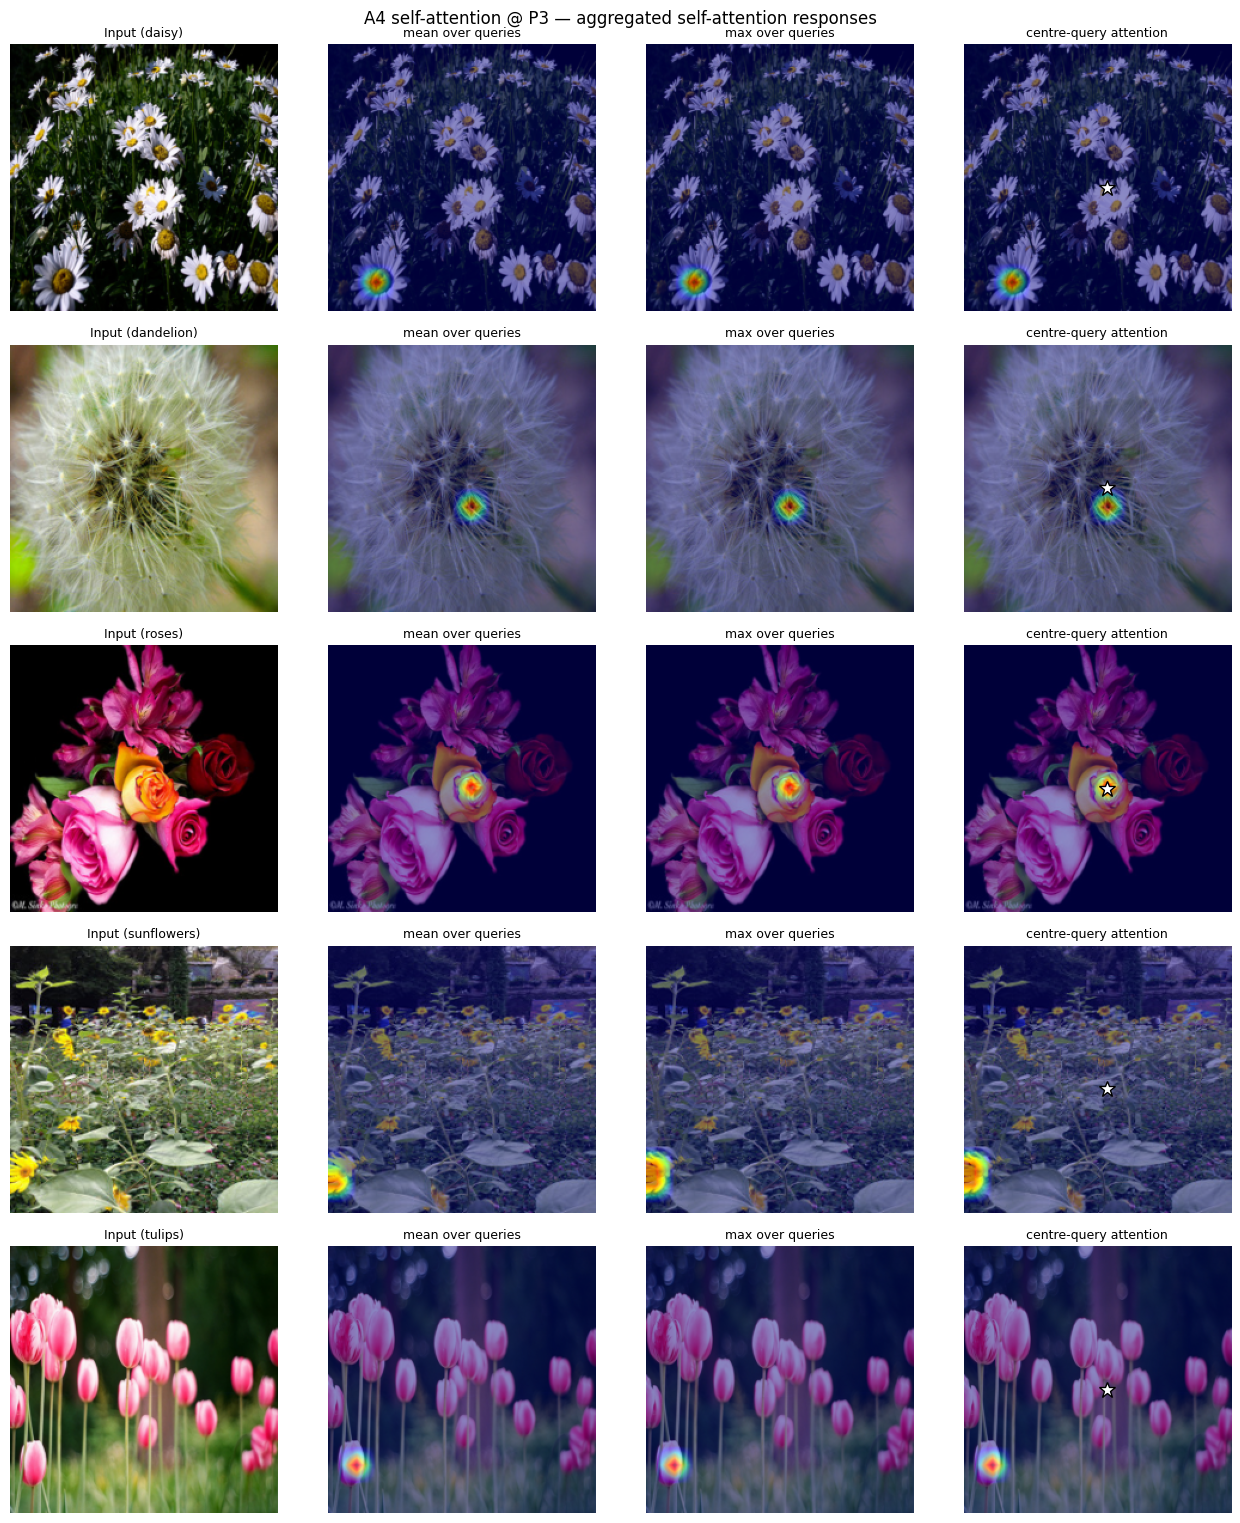
\includegraphics[width=0.80\textwidth]{plots/v_self_attention.png}
\caption{Self-attention (A4) at $P_3$ ($14\times14=196$ positions, $196\times196$ attention matrix): input, mean over queries, maximum over queries and attention of the centre query (star).}
\end{figure}

\textbf{Inference:} For every image the mean-over-queries, the maximum-over-queries and the centre-query maps show \emph{the same single compact hot-spot}, i.e.\ almost all query positions attend to the same location, including the centre query (marked by a star), whose attention does not stay at the star.
This agrees with the statistics over the whole test set: the normalised row entropy is only 0.0105 (very peaked rows) and the attention-weighted distance between a query and the positions it attends to is 6.35 cells, only slightly below the 7.28 expected for uniform attention. The location of the hot-spot depends on the image:
it falls on a daisy flower, on the centre of the dandelion and on one rose, whereas in the sunflowers and tulips images it falls at the bottom-left image corner (on a flower at the edge). The learned residual scale is small ($\gamma=0.0611$), so the response modifies the features only slightly. Distant regions therefore interact mainly through a few shared, image-dependent key positions rather than through a spatially varying pattern.

% ============================================================
\subsection*{29.4 Feature Maps Before and After Attention}
% ============================================================

Feature maps of the selected attention model (A4, $P_3$, $14\times14\times1024$) before and after the attention module for the first three representative images (test indices 1, 9 and 0): the mean over channels and the five channels with the highest mean activation before attention (channels 486, 513, 314, 908, 855).

\begin{figure}[H]
\centering
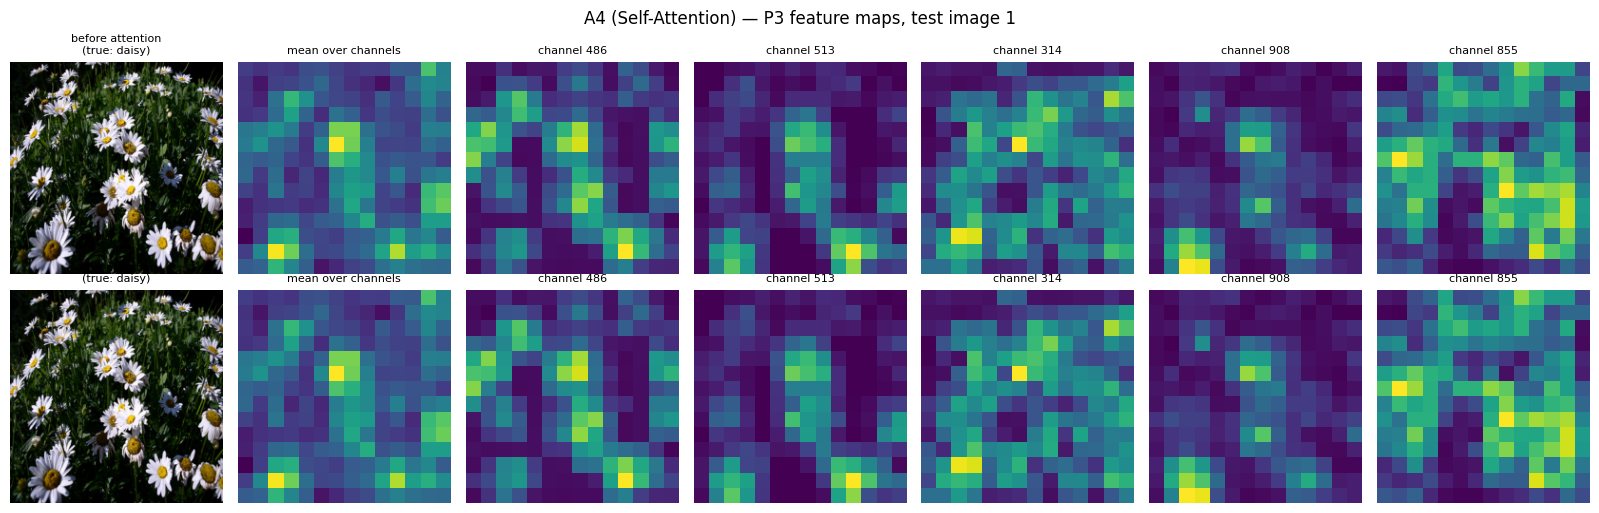
\includegraphics[width=0.98\textwidth]{plots/v_featuremaps_1.png}
\caption{Feature maps at $P_3$ of A4 before attention (top row) and after attention (bottom row) for the daisy image (test image 1). Further images: v\_featuremaps\_9 (dandelion) and v\_featuremaps\_0 (roses).}
\end{figure}

\begin{center}
\begin{tabular}{|l|c|c|c|c|}
\hline
\textbf{Test image} & \textbf{Mean $|$act.$|$ before} & \textbf{Mean $|$act.$|$ after} & \textbf{Mean act. before} & \textbf{Mean act. after} \\
\hline
1 (daisy) & 0.4793 & 0.7191 & 0.4793 & 0.4711 \\
\hline
9 (dandelion) & 0.4578 & 0.6029 & 0.4578 & 0.4451 \\
\hline
0 (roses) & 0.5238 & 0.7461 & 0.5238 & 0.5024 \\
\hline
\end{tabular}
\end{center}

\textbf{Inference:} The spatial pattern of the maps is almost unchanged by the attention module: the same hot-spots appear in the mean-over-channels map and in each of the five channels before and after attention. The numerical statistics show what the module does change:
the mean absolute activation increases by about 50\%, 32\% and 42\% (0.479 $\rightarrow$ 0.719, 0.458 $\rightarrow$ 0.603, 0.524 $\rightarrow$ 0.746) while the mean activation stays about the same or decreases slightly. Because the features before the module are non-negative (their mean equals their mean absolute value),
this means the self-attention residual $\gamma\,AV$ adds signed values, including negative ones, on top of the original features. The module thus refines the features by a small additive component, rather than by suppressing or amplifying whole regions.

% ============================================================
\section*{30. Attention Position Visualization}
% ============================================================

Use the same test image to visualize spatial attention at different ResNet50
stages.

Generate:

\[
M_s^{P_2},
\qquad
M_s^{P_3},
\qquad
M_s^{P_4}.
\]

Display the maps as:

\[
\boxed{
\text{Input}
\;|\;
M_s^{P_2}
\;|\;
M_s^{P_3}
\;|\;
M_s^{P_4}
}
\]

The objective is to visually study how attention changes as feature
representations become deeper.

Possible observations may include:

\begin{itemize}

\item $P_2$ responding strongly to edges, colors, textures, and fine
structures;

\item $P_3$ responding to flower parts and intermediate object structures;

\item $P_4$ responding to larger semantic flower regions.

\end{itemize}

These observations must be based on the student's experimental
visualizations.


Spatial-attention maps of the Channel$\rightarrow$Spatial models inserted at $P_2$ (B2, $28\times28$), $P_3$ (A3, $14\times14$) and $P_4$ (B4, $7\times7$), displayed for the five representative images.
The overlays are min--max normalised for display, so the raw range of each map is also given.

\begin{figure}[H]
\centering
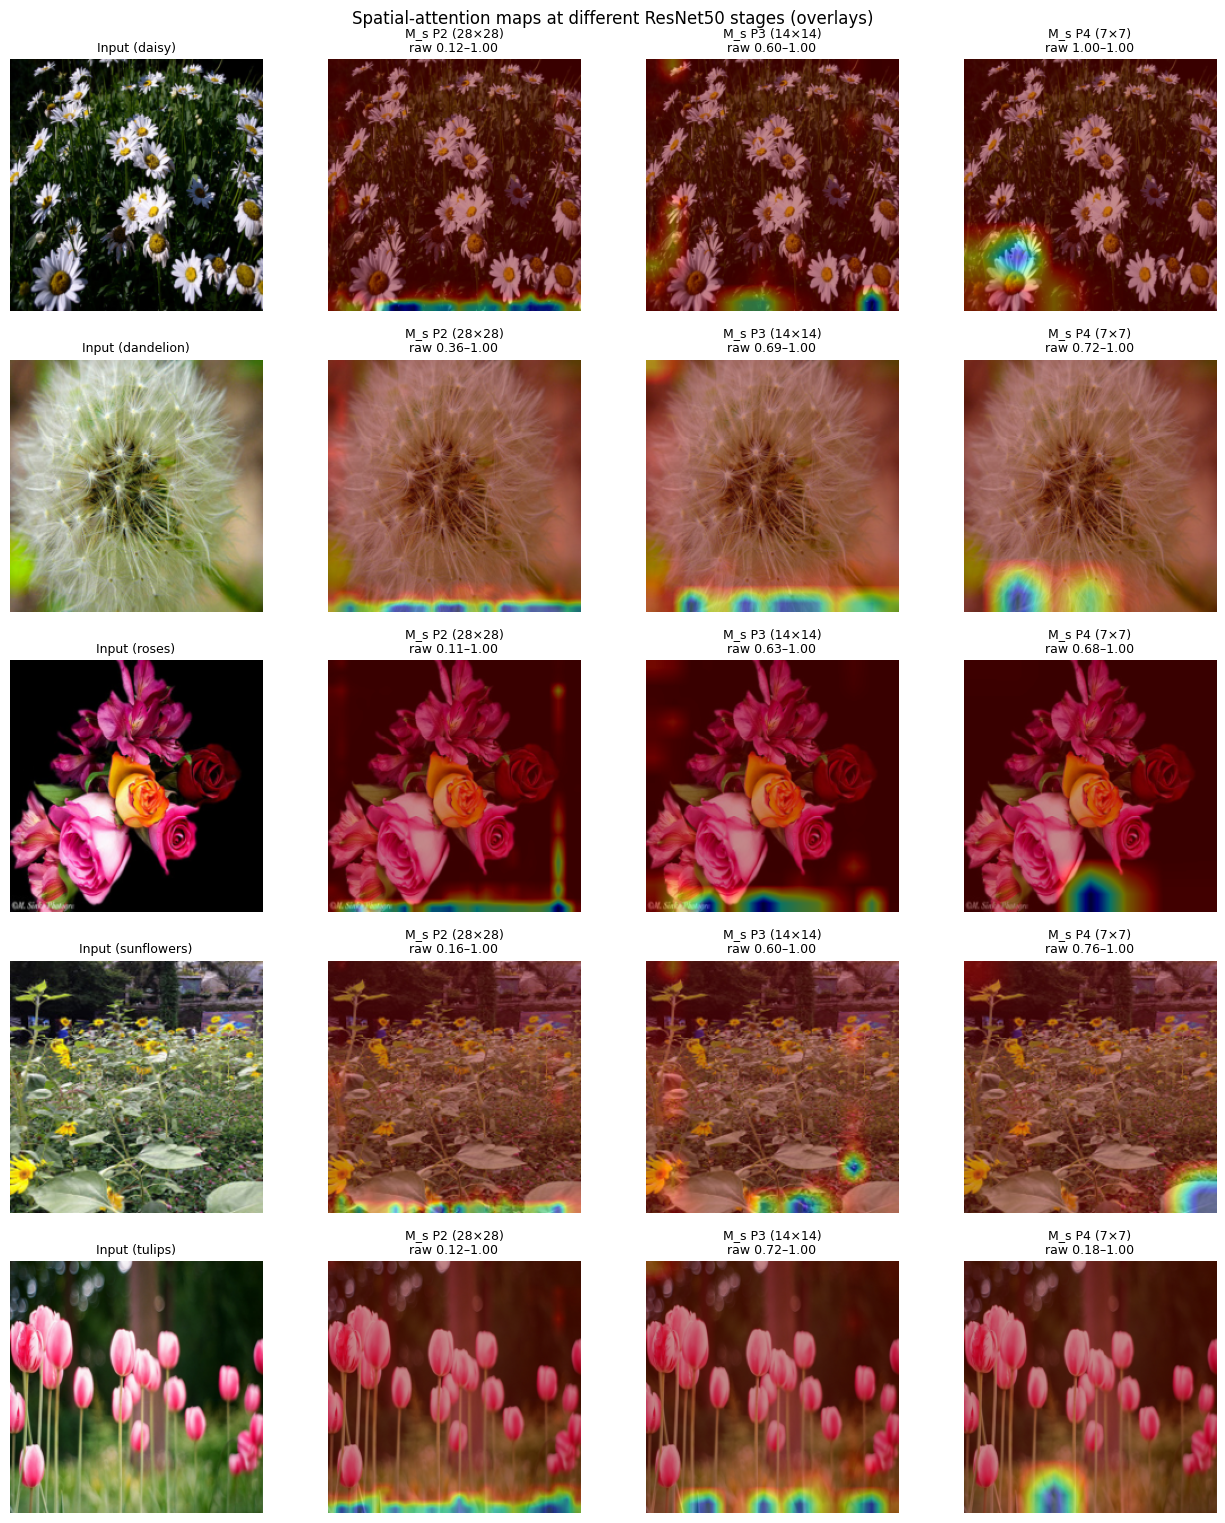
\includegraphics[width=0.85\textwidth]{plots/v_spatial_maps_P2_P3_P4.png}
\caption{Spatial-attention maps $M_s^{P_2}$, $M_s^{P_3}$, $M_s^{P_4}$ (overlays) for the five representative test images.}
\end{figure}

\begin{center}
\begin{tabular}{|l|c|c|c|}
\hline
\textbf{Image} & \textbf{raw range $P_2$} & \textbf{raw range $P_3$} & \textbf{raw range $P_4$} \\
\hline
daisy & 0.12--1.00 & 0.60--1.00 & 1.00--1.00 \\
\hline
dandelion & 0.36--1.00 & 0.69--1.00 & 0.72--1.00 \\
\hline
roses & 0.11--1.00 & 0.63--1.00 & 0.68--1.00 \\
\hline
sunflowers & 0.16--1.00 & 0.60--1.00 & 0.76--1.00 \\
\hline
tulips & 0.12--1.00 & 0.72--1.00 & 0.18--1.00 \\
\hline
\end{tabular}
\end{center}

\begin{center}
\begin{tabular}{|c|c|c|c|c|c|}
\hline
\textbf{Position} & \textbf{Model} & \textbf{Map size} & \textbf{Mean value} & \textbf{Std within map} & \textbf{\% positions $>0.5$} \\
\hline
$P_2$ & B2 & $28\times28$ & 0.9776 & 0.0898 & 98.71 \\
\hline
$P_3$ & A3 & $14\times14$ & 0.9860 & 0.0425 & 99.93 \\
\hline
$P_4$ & B4 & $7\times7$ & 0.9905 & 0.0376 & 99.57 \\
\hline
\end{tabular}
\end{center}

\textbf{Inference:} At all three stages the maps are close to 1 over most of the image and the lowest values are located near the bottom border (a thin strip at $P_2$, small patches at $P_3$, larger coarse blocks at $P_4$) rather than on the flowers; the maps do not follow the flower in any of the five images.
The resolution of the map changes with depth, as expected ($28\times28$ gives fine detail, $7\times7$ blocky regions), and the maps become more uniform with depth (mean 0.978 $\rightarrow$ 0.986 $\rightarrow$ 0.991; standard deviation within the map 0.090 $\rightarrow$ 0.043 $\rightarrow$ 0.038). The raw range shows that the apparent structure
of the $P_4$ overlays is partly an effect of normalisation: for the daisy image the raw $P_4$ map is constant (1.00--1.00) and for most other images its minimum is 0.68--0.76. We therefore did not observe a clear shift of the spatial attention from edges and textures at $P_2$ to flower parts at $P_3$ and larger flower regions at $P_4$; instead the learned spatial maps are almost saturated at all depths.

% ============================================================
\section*{31. Qualitative Comparison Across Attention Mechanisms}
% ============================================================

Select at least:

\[
\boxed{
3\text{ correctly classified images}
}
\]

and

\[
\boxed{
2\text{ incorrectly classified images}.
}
\]

For every selected image, compare the behavior of multiple models.

A recommended arrangement is:

\[
\boxed{
\begin{array}{c}
\text{Input Image}\\
\downarrow\\
\text{Baseline Grad-CAM}\\
\text{Channel-Attention Grad-CAM}\\
\text{Spatial-Attention Map}\\
\text{Channel+Spatial Grad-CAM}\\
\text{Self-Attention Response}
\end{array}
}
\]

Students may alternatively arrange the images horizontally in the report.


Three test images correctly classified by the baseline and by the selected model A4 (indices 188 dandelion, 300 roses, 79 sunflowers) and two images misclassified by the selected model A4 (index 69 sunflowers, index 157 daisy; 31 misclassified images were available) were chosen with a fixed random seed.

\begin{center}
\resizebox{\textwidth}{!}{
\begin{tabular}{|c|c|l|c|c|c|c|c|c|}
\hline
\textbf{Test idx} & \textbf{Group} & \textbf{True} & \textbf{A0} & \textbf{A1} & \textbf{A2} & \textbf{A3} & \textbf{A4} & \textbf{A5} \\
\hline
188 & correct & dandelion & dandelion & dandelion & dandelion & dandelion & dandelion & dandelion \\
\hline
300 & correct & roses & roses & roses & roses & roses & roses & roses \\
\hline
79 & correct & sunflowers & sunflowers & sunflowers & sunflowers & sunflowers & sunflowers & sunflowers \\
\hline
69 & incorrect & sunflowers & sunflowers & sunflowers & sunflowers & sunflowers & dandelion & sunflowers \\
\hline
157 & incorrect & daisy & dandelion & daisy & dandelion & daisy & dandelion & daisy \\
\hline
\end{tabular}}
\end{center}

\begin{figure}[H]
\centering
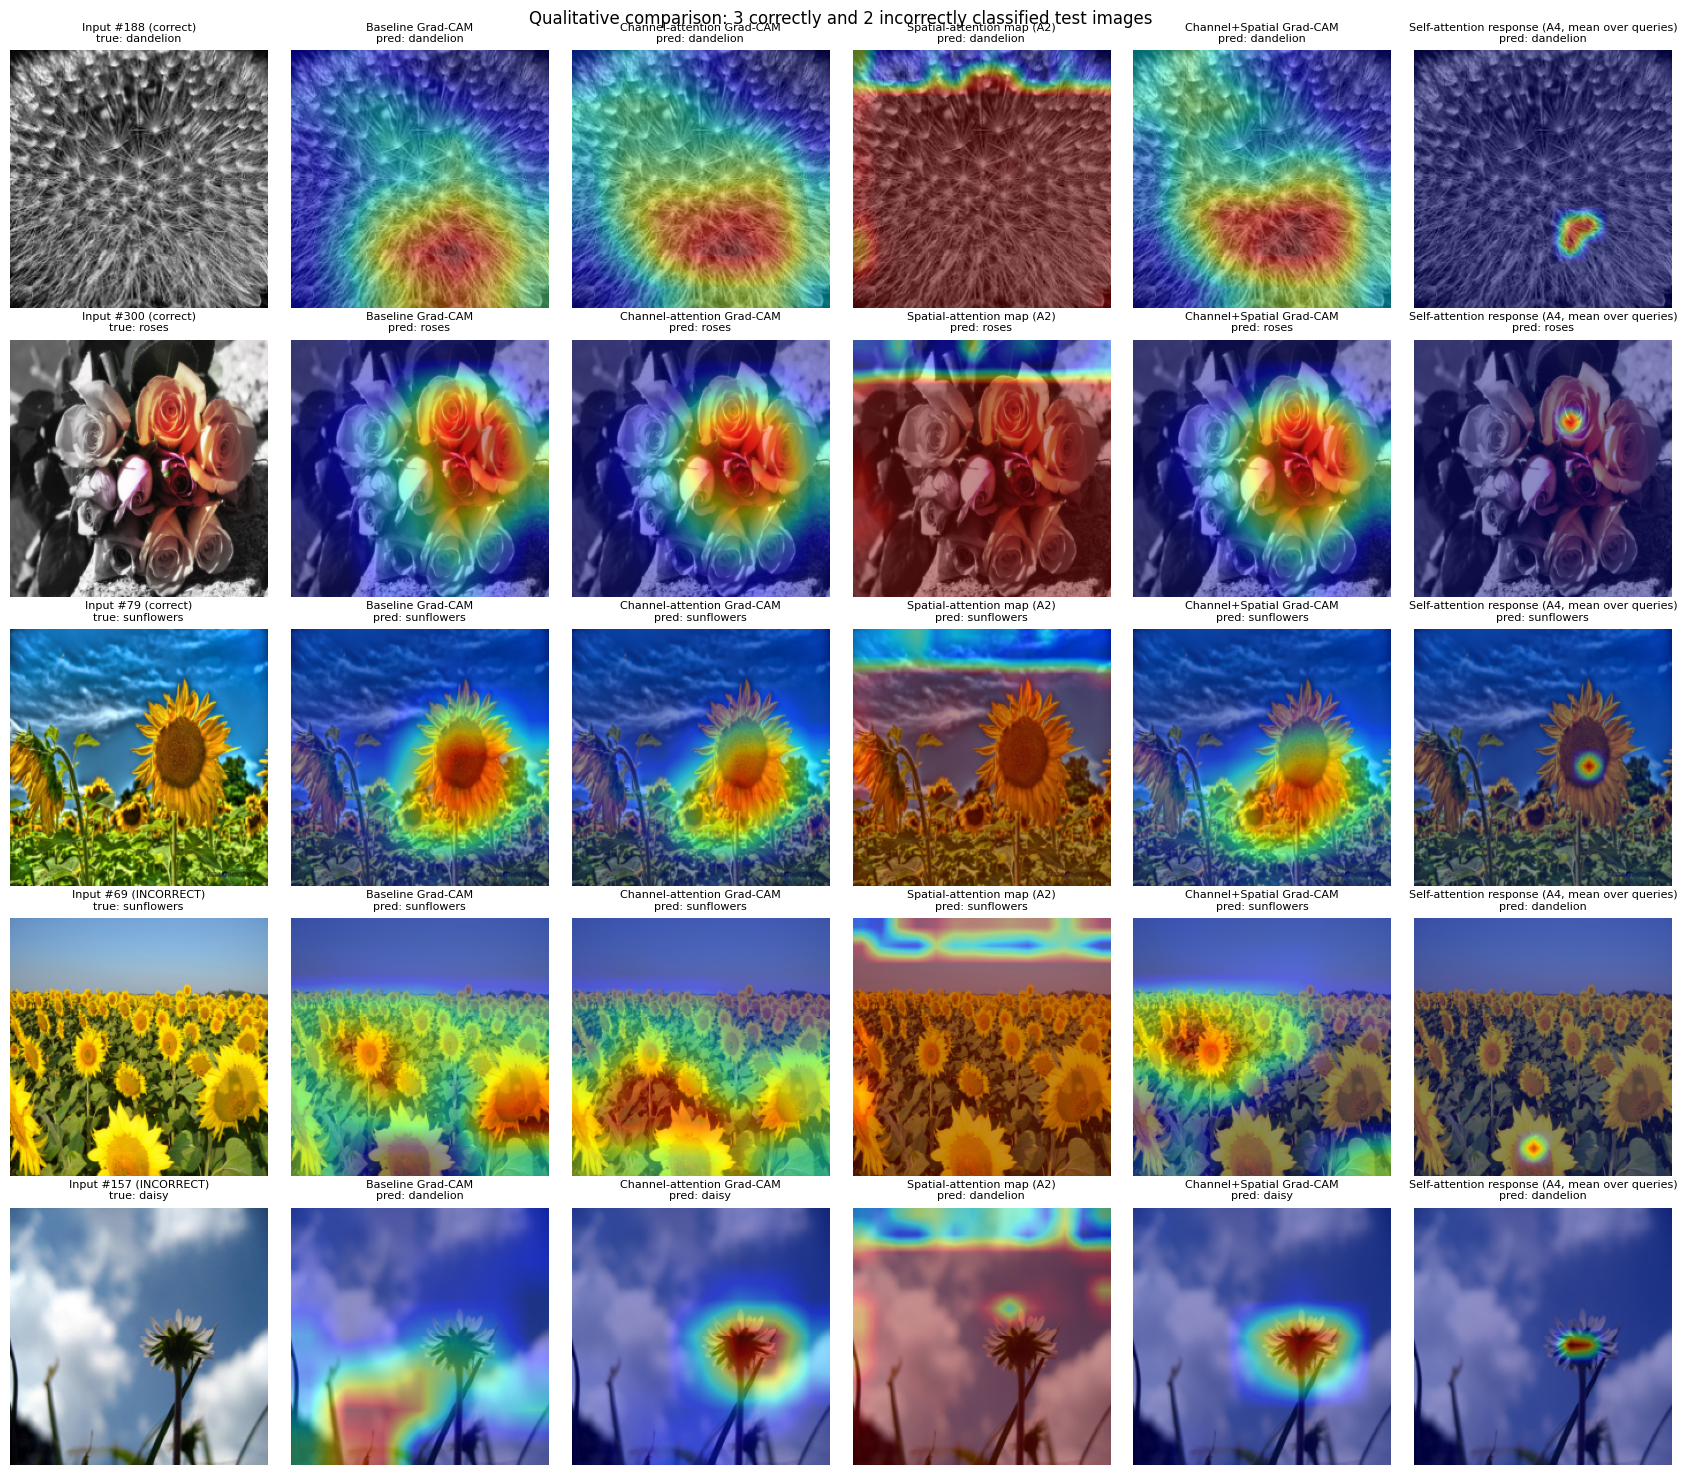
\includegraphics[width=0.98\textwidth]{plots/v_qualitative_comparison.png}
\caption{Input, baseline Grad-CAM, channel-attention Grad-CAM, spatial-attention map (A2), channel+spatial Grad-CAM and self-attention response (A4) for three correctly (rows 1--3) and two incorrectly (rows 4--5) classified test images.}
\end{figure}

\begin{center}
\resizebox{\textwidth}{!}{
\begin{tabular}{|c|c|c|c|c|c|c|}
\hline
\textbf{Test idx} & \textbf{Cov. A0} & \textbf{Ent. A0} & \textbf{Cov. A1} & \textbf{Ent. A1} & \textbf{Cov. A3} & \textbf{Ent. A3} \\
\hline
188 (correct) & 0.2684 & 0.9289 & 0.3448 & 0.9474 & 0.2962 & 0.9454 \\
\hline
300 (correct) & 0.2187 & 0.8653 & 0.1959 & 0.8442 & 0.2051 & 0.8247 \\
\hline
79 (correct) & 0.1685 & 0.8072 & 0.1263 & 0.7633 & 0.1397 & 0.8057 \\
\hline
69 (incorrect for A4) & 0.2676 & 0.8864 & 0.3534 & 0.8916 & 0.1484 & 0.7827 \\
\hline
157 (incorrect for A0, A2, A4) & 0.1474 & 0.8125 & 0.0916 & 0.7155 & 0.0718 & 0.4846 \\
\hline
\end{tabular}}
\end{center}

\textbf{Inference:} \textbf{Correct images.} In the dandelion, roses and sunflowers images the baseline, channel and channel+spatial Grad-CAMs peak on the flower (lower-centre of the dandelion head, the central cluster of roses, the large sunflower), and the self-attention response is one hot-spot on the flower (dandelion head, one rose, sunflower disc).
The spatial-attention map of A2 is nearly uniform apart from a strip along the top border. The attention models change the extent of the Grad-CAM (coverage for the dandelion 0.268 $\rightarrow$ 0.345, 0.296 broader; for the sunflower 0.169 $\rightarrow$ 0.126, 0.140 more compact) but not its location.
\textbf{Incorrect images.} In the sunflower-field image (index 69) only A4 is wrong (it predicts dandelion); the Grad-CAMs of A0, A1 and A3 are spread over several flower heads and the foreground of a scene with many small sunflowers and no single dominant flower, and the A4 self-attention hot-spot lies on one sunflower head.
In the daisy image (index 157) the baseline is wrong (dandelion) and its Grad-CAM lies at the lower left, away from the flower head, whereas the channel and channel+spatial models classify it correctly and their Grad-CAMs are centred on the flower head and much more compact (coverage 0.147 $\rightarrow$ 0.092 and 0.072; entropy 0.813 $\rightarrow$ 0.716 and 0.485);
A4 is wrong here although its self-attention hot-spot is on the flower head, so attending to the flower did not guarantee a correct prediction. These are two examples; the conclusions on correct versus incorrect samples are therefore supported by the whole-test-set statistics below.

% ============================================================
\subsection*{31.1 Qualitative Criteria}
% ============================================================

The student should discuss:

\begin{itemize}

\item foreground localization;

\item background suppression;

\item localization of petals;

\item localization of the flower center;

\item activation compactness;

\item activation coverage;

\item incorrectly attended regions;

\item differences between correctly and incorrectly classified samples;

\item differences between shallow and deep attention; and

\item consistency of attention across different images.

\end{itemize}


\textbf{Measured Grad-CAM statistics over the whole test set, correctly versus incorrectly classified images (every model).}

\begin{center}
\resizebox{\textwidth}{!}{
\begin{tabular}{|c|l|c|c|c|c|c|c|c|}
\hline
\textbf{ID} & \textbf{Model} & \textbf{Pos.} & \textbf{\# corr.} & \textbf{\# incorr.} & \textbf{Cov. corr.} & \textbf{Cov. incorr.} & \textbf{Ent. corr.} & \textbf{Ent. incorr.} \\
\hline
A0 & Baseline ResNet50 & -- & 524 & 27 & 0.2400 & 0.1471 & 0.8449 & 0.7893 \\
\hline
A1 & Channel Attention (SE-style) & P3 & 521 & 30 & 0.2137 & 0.1443 & 0.8298 & 0.7686 \\
\hline
A2 & Spatial Attention ($7\times7$) & P3 & 505 & 46 & 0.1874 & 0.0960 & 0.8254 & 0.7316 \\
\hline
A3 & Channel+Spatial (C$\rightarrow$S) & P3 & 512 & 39 & 0.2091 & 0.1203 & 0.8313 & 0.7330 \\
\hline
A4 & Self-Attention & P3 & 520 & 31 & 0.2808 & 0.1569 & 0.8906 & 0.8368 \\
\hline
A5 & Combined (C$\rightarrow$S$\rightarrow$Self) & P3 & 507 & 44 & 0.3155 & 0.2034 & 0.9071 & 0.8361 \\
\hline
B1 & Channel+Spatial (C$\rightarrow$S) & P1 & 502 & 49 & 0.1903 & 0.1197 & 0.8248 & 0.7792 \\
\hline
B2 & Channel+Spatial (C$\rightarrow$S) & P2 & 519 & 32 & 0.1980 & 0.1198 & 0.8126 & 0.7333 \\
\hline
B4 & Channel+Spatial (C$\rightarrow$S) & P4 & 523 & 28 & 0.2541 & 0.1718 & 0.9046 & 0.8766 \\
\hline
C1 & Channel+Spatial (C$\rightarrow$S) & P3+P4 & 514 & 37 & 0.2440 & 0.1827 & 0.8747 & 0.8207 \\
\hline
C2 & Channel+Spatial (C$\rightarrow$S) & P2+P3+P4 & 510 & 41 & 0.2175 & 0.1398 & 0.8565 & 0.7846 \\
\hline
D1 & Spatial$\rightarrow$Channel (S$\rightarrow$C) & P3 & 523 & 28 & 0.2254 & 0.1669 & 0.8379 & 0.7690 \\
\hline
E1 & Spatial Attention ($3\times3$) & P3 & 523 & 28 & 0.1974 & 0.1399 & 0.8412 & 0.8244 \\
\hline
E2 & Spatial Attention ($5\times5$) & P3 & 511 & 40 & 0.1717 & 0.1156 & 0.8205 & 0.8035 \\
\hline
F1 & ECA & P3 & 508 & 43 & 0.1964 & 0.1378 & 0.8197 & 0.7651 \\
\hline
F2 & CBAM & P3 & 506 & 45 & 0.1884 & 0.1043 & 0.8106 & 0.6993 \\
\hline
\end{tabular}}
\end{center}

\textbf{Inference:} \textbf{Foreground localization and background suppression:} on the representative images the strongest activation lies on the flower for all models, but the field images (daisy, sunflowers) show activation over a large part of the scene, and no model shows a clear suppression of background.
\textbf{Compactness and coverage:} coverage is lowest for spatial attention (0.1798) and highest for the combined model (0.3065); a more compact Grad-CAM was not associated with higher accuracy (the $P_4$ model, with coverage 0.2499 and entropy 0.9032, is the most accurate position).
\textbf{Correct versus incorrect samples:} for every one of the 16 models the Grad-CAM of misclassified images has a smaller coverage and a lower entropy than that of correctly classified images (for example baseline 0.147 versus 0.240 and 0.789 versus 0.845; A4 0.157 versus 0.281 and 0.837 versus 0.891), i.e.\ errors tend to occur when the explanation is concentrated on a smaller region.
\textbf{Shallow versus deep attention:} the internal maps are fine-grained but almost saturated at $P_2$ and coarse and almost saturated at $P_4$ (Section 30).
\textbf{Consistency across images:} the channel weights are nearly identical for different images (correlation 0.997) and the spatial maps share the same border pattern for all images, so the internal attention is highly consistent, mostly input-independent.

% ============================================================
\section*{32. Required Visualizations}
% ============================================================

The laboratory report must contain the following visualizations:

\begin{enumerate}

\item sample input images from all five classes;

\item training and validation accuracy curves;

\item training and validation loss curves;

\item confusion matrix;

\item feature map before attention;

\item channel-attention weights;

\item spatial-attention heatmap;

\item spatial-attention overlay;

\item self-attention response for the self-attention experiment;

\item feature map after attention;

\item baseline Grad-CAM;

\item Grad-CAM for at least one attention-based model;

\item attention maps at $P_2$, $P_3$, and $P_4$; and

\item at least one graphical comparison of the performances of different
attention mechanisms.

\end{enumerate}


Location of each required visualization in this report (file names are the names under which the notebook saved the figures; the figure placeholders in the report use the same names).

\begin{center}
\small
\begin{tabular}{|c|p{5.2cm}|p{6.2cm}|l|}
\hline
\textbf{\#} & \textbf{Visualization} & \textbf{Figure file(s)} & \textbf{Report section} \\
\hline
1 & Sample input images of all five classes & \texttt{v01\_sample\_images} & Section 3.2 \\
\hline
2 & Training and validation accuracy curves & \texttt{v\_curves\_accuracy\_exp1}, \texttt{v\_curves\_accuracy\_exp2} & Section 25.1 \\
\hline
3 & Training and validation loss curves & \texttt{v\_curves\_loss\_exp1}, \texttt{v\_curves\_loss\_exp2} & Section 25.2 \\
\hline
4 & Confusion matrix (baseline and selected A4) & \texttt{v\_confusion\_matrices} & Section 26 \\
\hline
5 & Feature map before attention & \texttt{v\_featuremaps\_1} (also \_9, \texttt{\_0)} & Section 29.4 \\
\hline
6 & Channel-attention weights & \texttt{v\_channel\_weights\_A1}, \texttt{v\_channel\_weights\_A3} & Section 29.1 \\
\hline
7 & Spatial-attention heatmap & \texttt{v\_spatial\_maps\_A2}, \texttt{v\_spatial\_maps\_A3} & Section 29.2 \\
\hline
8 & Spatial-attention overlay & \texttt{v\_spatial\_maps\_A2}, \texttt{v\_spatial\_maps\_A3} & Section 29.2 \\
\hline
9 & Self-attention response & \texttt{v\_self\_attention} & Section 29.3 \\
\hline
10 & Feature map after attention & \texttt{v\_featuremaps\_1} (bottom row) & Section 29.4 \\
\hline
11 & Baseline Grad-CAM & \texttt{v\_gradcam\_layout} & Section 28 \\
\hline
12 & Grad-CAM of attention models & \texttt{v\_gradcam\_layout}, \texttt{v\_qualitative\_comparison} & Sections 28, 31 \\
\hline
13 & Attention maps at $P_2$, $P_3$, $P_4$ & \texttt{v\_spatial\_maps\_P2\_P3\_P4} & Section 30 \\
\hline
14 & Graphical comparison of attention mechanisms & \texttt{v\_bar\_mech\_accuracy}, \texttt{v\_bar\_mech\_f1}, \texttt{v\_bar\_position}, \texttt{v\_scatter\_tradeoffs} & Sections 25.3--25.6 \\
\hline
\end{tabular}
\end{center}

% ============================================================
\section*{33. Recommended Visualization Layout}
% ============================================================

For one representative test image, students are encouraged to generate a
figure in the following format:

\[
\boxed{
\begin{array}{ccccc}
\text{Input}
&
\text{Baseline}
&
\text{Channel}
&
\text{Spatial}
&
\text{Channel+Spatial}
\\
&
\text{Grad-CAM}
&
\text{Grad-CAM}
&
\text{Attention Map}
&
\text{Grad-CAM}
\end{array}
}
\]

For students completing the additional attention comparison, the figure may
be extended to:

\[
\boxed{
\text{Input}
|
\text{Baseline}
|
\text{SE}
|
\text{ECA}
|
\text{CBAM}
|
\text{Self-Attention}
}
\]

using appropriate visualization methods.


The recommended layout (Input $|$ Baseline Grad-CAM $|$ Channel Grad-CAM $|$ Spatial attention map $|$ Channel+Spatial Grad-CAM, extended with the self-attention response) was produced for the five representative test images in
\texttt{v\_gradcam\_layout} (Section 28) and for the five selected correct/incorrect images in \texttt{v\_qualitative\_comparison} (Section 31). Grad-CAM panels were generated for A0, A1, A3 and A4 (and A2/A4 internal maps) only; for ECA and CBAM, which were not retained for visualization, only the quantitative
and measured Grad-CAM statistics are available (Section 20.1).

% ============================================================
\section*{34. Required Experimental Analysis}
% ============================================================

The final report should contain three forms of analysis.

\subsection*{34.1 Quantitative Analysis}

Report:

\[
\boxed{
\text{Accuracy}
+
\text{Precision}
+
\text{Recall}
+
\text{Macro F1}
}
\]

\subsection*{34.2 Complexity Analysis}

Report:

\[
\boxed{
\text{Parameters}
+
\text{Inference Time}
}
\]

\subsection*{34.3 Qualitative Analysis}

Report:

\[
\boxed{
\text{Grad-CAM}
+
\text{Attention Maps}
+
\text{Visual Interpretation}
}
\]

Therefore, the overall evaluation should be:

\[
\boxed{
\text{Quantitative}
+
\text{Computational}
+
\text{Qualitative}
}
\]


Accuracy, precision, recall and macro F1 of all 16 models are given in Sections 15--20 and 24 and Section 39. Best test accuracy: baseline 0.9510; best attention models: Channel+Spatial at $P_4$ (B4), Spatial$\rightarrow$Channel at $P_3$ (D1) and spatial $3\times3$ (E1), all 0.9492 (523 of 551 correct); the best macro F1 among the attention models is E1 (0.9500), followed by B4 (0.9499) and D1 (0.9489).


Total parameters range from 23{,}597{,}957 (baseline) to 25{,}040{,}937 (combined) and inference time from 3.904 to 4.276 ms per image (Sections 15--20). The three most accurate attention models add 19 parameters (E1; 3.951 ms), 132{,}259 parameters (D1; 3.982 ms) and 526{,}563 parameters (B4; 3.981 ms);
the heaviest models (self-attention and combined, +1.3--1.4M parameters) are also the slowest.


Grad-CAM maps are broadly similar between the baseline and the attention models, differing mainly in coverage (Sections 28, 31); the internal spatial maps are almost saturated and show a border pattern, the channel weights are nearly input-independent, and the self-attention response is a single hot-spot (Section 29);
the spatial maps do not change character with depth (Section 30).

% ============================================================
\section*{35. Experimental Protocol}
% ============================================================

To ensure fair comparison, all ablation experiments must use:

\begin{itemize}

\item identical training images;

\item identical validation images;

\item identical testing images;

\item identical random seed where possible;

\item identical image preprocessing;

\item identical augmentation;

\item identical backbone;

\item identical classifier;

\item identical optimizer;

\item identical batch size;

\item identical number of epochs;

\item identical learning-rate schedule;

\item identical fine-tuning procedure; and

\item identical evaluation metrics.

\end{itemize}

Only the experimental factor under investigation should change.

For example, when studying attention position:

\[
\boxed{
\text{Only Attention Position Should Change}
}
\]

and when studying attention type:

\[
\boxed{
\text{Only Attention Type Should Change}.
}
\]

% ============================================================
\section*{36. Minimum Mandatory Ablation Set}
% ============================================================

If laboratory time is limited, every student must complete at least the
following experiments:

\begin{enumerate}

\item Baseline pretrained ResNet50.

\item Channel attention at $P_3$.

\item Spatial attention at $P_3$.

\item Channel+Spatial attention at $P_3$.

\item Channel+Spatial attention at $P_2$.

\item Channel+Spatial attention at $P_4$.

\item Self-attention at $P_3$.

\item Grad-CAM comparison between baseline ResNet50 and one selected
attention model.

\item Spatial-attention visualization at $P_2$, $P_3$, and $P_4$.

\item Graphical comparison of the classification performance of the attention
models.

\end{enumerate}

This minimum set allows students to study:

\[
\boxed{\text{Attention Type}}
\]

and

\[
\boxed{\text{Attention Position}}.
\]


All ten items of the minimum set were completed: baseline (A0), channel (A1), spatial (A2) and channel+spatial (A3) attention at $P_3$, channel+spatial at $P_2$ (B2) and $P_4$ (B4), self-attention at $P_3$ (A4),
the Grad-CAM comparison between the baseline and attention models (Section 28), the spatial-attention visualization at $P_2$, $P_3$ and $P_4$ (Section 30) and the graphical comparison of the attention models (Section 25). In addition, the extended experiments
($P_1$, $P_3+P_4$, $P_2+P_3+P_4$, Spatial$\rightarrow$Channel, kernel sizes $3\times3$ and $5\times5$, ECA and CBAM) were performed.

% ============================================================
\section*{37. Additional Student Exploration}
% ============================================================

Students interested in extended experimentation should select at least two
mechanisms from:

\[
\boxed{
\text{SE},
\quad
\text{ECA},
\quad
\text{CBAM},
\quad
\text{Coordinate Attention},
\quad
\text{Self-Attention}
}
\]

and integrate them with the same ResNet50 backbone.

Students should maintain the same:

\begin{itemize}

\item dataset split;

\item preprocessing;

\item augmentation;

\item optimizer;

\item epochs;

\item fine-tuning strategy; and

\item attention position.

\end{itemize}

The additional investigation should include both:

\[
\boxed{
\text{Quantitative Comparison}
}
\]

and

\[
\boxed{
\text{Qualitative Comparison}.
}
\]


Two additional mechanisms, ECA and CBAM, were integrated with the same ResNet50 backbone at $P_3$ under the same dataset split, preprocessing, augmentation, optimizer, epochs and fine-tuning strategy; SE corresponds to the SE-style channel module (A1) and self-attention to A4.
The quantitative comparison is given in Section 20.1 (ECA 0.9220, CBAM 0.9183 test accuracy). Qualitatively, only measured statistics are available for ECA and CBAM (ECA channel weights: mean 0.523, std 0.077; Grad-CAM coverage 0.1919, entropy 0.8154; CBAM Grad-CAM coverage 0.1816, entropy 0.8015);
Grad-CAM panels and internal-map figures were produced only for A0--A5, B2 and B4. Coordinate attention was not implemented.

% ============================================================
\section*{38. Questions Students Must Answer}
% ============================================================

\begin{enumerate}

\item What is the purpose of residual connections in ResNet50?\\
\textbf{Answer:} Residual (skip) connections add a block's input to its output, so each block learns a residual and gradients can flow through the identity path; this allows a 50-layer network to be trained without degradation.

\item What does conv2\_x represent compared with conv5\_x?\\
\textbf{Answer:} conv2\_x is an early stage ($56\times56\times256$) that encodes edges, colours and simple textures; conv5\_x is the last stage ($7\times7\times2048$) that encodes high-level, class-discriminative semantic information.

\item Why does the spatial resolution decrease with network depth?\\
\textbf{Answer:} Strides and pooling downsample the feature map from stage to stage ($56\times56\rightarrow28\times28\rightarrow14\times14\rightarrow7\times7$), which enlarges the receptive field and reduces the computation of the deeper layers.

\item Why does the number of feature channels increase with network depth?\\
\textbf{Answer:} The channels increase ($256\rightarrow512\rightarrow1024\rightarrow2048$) so that deeper layers can represent a larger variety of increasingly abstract patterns while the spatial resolution shrinks.

\item What is meant by low-level, intermediate, and high-level features?\\
\textbf{Answer:} Low-level features are edges, colours and simple textures (early stages); intermediate features are local patterns and parts such as petal arrangements; high-level features are object-level, class-discriminative structures (late stages).

\item What is the purpose of an attention mechanism?\\
\textbf{Answer:} An attention mechanism re-weights features so that the network emphasises informative channels, locations or positions and down-weights less useful ones.

\item What does channel attention attempt to learn?\\
\textbf{Answer:} It learns an importance weight for each channel (which feature channels matter) from the globally pooled descriptor; in A1 the 1024 weights ranged from 0.0018 to 0.9993 and about 600 were above 0.5.

\item What does spatial attention attempt to learn?\\
\textbf{Answer:} It learns an importance weight for each spatial location from the channel-wise mean and max maps (where the informative regions are); in A2 the map had mean 0.885 and 87.3\% of the positions were above 0.5.

\item How is channel attention different from spatial attention?\\
\textbf{Answer:} Channel attention gives one weight per channel shared over all positions (``what''), whereas spatial attention gives one weight per position shared over all channels (``where'').

\item Why can channel and spatial attention be used sequentially?\\
\textbf{Answer:} Both modules preserve the $H\times W\times C$ shape, so the output of one is a valid input of the other and the two complementary kinds of re-weighting can be chained (A3: C$\rightarrow$S, D1: S$\rightarrow$C, and CBAM).

\item Why might channel attention behave differently at conv3\_x and
conv5\_x?\\
\textbf{Answer:} At conv3\_x ($28\times28\times512$) the features are mid-level, at conv5\_x ($7\times7\times2048$) they are semantic and have four times more channels. Measured: the mean channel weight is 0.635 at $P_2$ but 0.483 at $P_4$ (more channels suppressed at the deeper stage), and the module has 33{,}411 parameters at $P_2$ versus 526{,}563 at $P_4$.

\item Why can spatial attention be useful at an intermediate ResNet stage?\\
\textbf{Answer:} An intermediate stage keeps enough spatial resolution and enough semantic content for a spatial map to be meaningful. In this experiment, however, the spatial maps at $P_2$ and $P_3$ were almost saturated (mean 0.978 and 0.986), so the good accuracy at $P_2$ (0.9419) cannot be attributed to the spatial component alone.

\item Why is self-attention computationally expensive when the feature map
has high spatial resolution?\\
\textbf{Answer:} Self-attention computes a score for every pair of positions, so memory and computation grow with the square of the number of positions $N=H\times W$.

\item What happens to the size of the self-attention matrix when the spatial
resolution increases?\\
\textbf{Answer:} The attention matrix is $N\times N$ with $N=HW$: $196\times196=38{,}416$ entries at $P_3$ ($14\times14$), $784\times784=614{,}656$ at $P_2$ ($28\times28$) and $3136\times3136=9{,}834{,}496$ at $P_1$ ($56\times56$) per image, i.e.\ quadratic growth with the number of positions.

\item How does attention performance vary when the insertion position is
changed?\\
\textbf{Answer:} It changes it considerably: with Channel$\rightarrow$Spatial the test accuracy was 0.9111 ($P_1$), 0.9419 ($P_2$), 0.9292 ($P_3$) and 0.9492 ($P_4$); the shallowest position was worst and the deepest best, but not monotonically.

\item How does attention at $P_2$ differ visually from attention at $P_4$?\\
\textbf{Answer:} At $P_2$ the map is $28\times28$ with a thin low-value strip along the bottom edge; at $P_4$ it is $7\times7$ with larger, blocky low-value regions near the bottom. Both are almost saturated (mean 0.978 versus 0.990), and neither follows the flowers (Section 30).

\item Does applying attention at multiple stages always improve
classification performance?\\
\textbf{Answer:} No: $P_3+P_4$ (0.9328) and $P_2+P_3+P_4$ (0.9256) were less accurate than $P_4$ alone (0.9492) while using more parameters, training time and inference time.

\item Does Channel$\rightarrow$Spatial attention behave differently from
Spatial$\rightarrow$Channel attention?\\
\textbf{Answer:} Yes, in this run: Spatial$\rightarrow$Channel reached 0.9492 and Channel$\rightarrow$Spatial 0.9292 with identical parameters; the spatial map is also less saturated when computed first (mean 0.936 versus 0.986). Single run, so this should be confirmed with other seeds.

\item How does the spatial-attention kernel size influence the attention map?\\
\textbf{Answer:} A larger kernel produced a less saturated, more selective map (mean 0.983, 0.903, 0.885 and fraction above 0.5 of 99.9\%, 91.4\%, 87.3\% for $3\times3$, $5\times5$, $7\times7$), and the accuracy decreased (0.9492, 0.9274, 0.9165).

\item How does SE attention differ from ECA attention?\\
\textbf{Answer:} SE uses global average pooling and two fully connected layers with reduction ratio 16 (132{,}160 parameters at $C=1024$); ECA uses a 1-D convolution of adaptive kernel size (5 for $C=1024$) over the channel descriptor without dimension reduction (5 parameters). Here SE-style reached 0.9456 and ECA 0.9220.

\item How does CBAM combine channel and spatial attention?\\
\textbf{Answer:} CBAM applies channel attention (average- and max-pooled descriptors through a shared MLP) followed by $7\times7$ spatial attention; it has the same number of parameters as A3 (132{,}259) but reached 0.9183 versus 0.9292 for A3.

\item How does self-attention differ from channel attention?\\
\textbf{Answer:} Channel attention weights channels from a pooled descriptor with no interaction between positions, whereas self-attention relates every pair of positions (a $196\times196$ matrix at $P_3$) and adds 1{,}310{,}721 parameters versus 132{,}160; its learned $\gamma$ was 0.0611 and its rows were very peaked (entropy 0.0105).

\item Does the attention mechanism with the largest number of parameters
necessarily provide the highest accuracy?\\
\textbf{Answer:} No: the combined model (1{,}442{,}980 attention parameters) reached 0.9201, self-attention (1{,}310{,}721) 0.9437, SE-style channel (132{,}160) 0.9456 and the baseline (0) 0.9510.

\item What is the difference between an internal attention map and Grad-CAM?\\
\textbf{Answer:} An internal attention map is computed by the module during the forward pass and directly re-weights the features (for example the spatial map $M_s$ or the channel weights), whereas Grad-CAM is computed afterwards from the gradient of a class score with respect to a feature map. In this experiment they differ visibly: the $P_3$ spatial maps are almost saturated with low values at the borders, while Grad-CAM highlights flower regions.

\item Why is Grad-CAM called a post-hoc explanation technique?\\
\textbf{Answer:} Because it is generated after the prediction, from the gradients of the already trained model, and neither changes the model nor takes part in training.

\item Does the attention model suppress irrelevant background regions?\\
\textbf{Answer:} Not clearly: the spatial maps are almost saturated and their low values lie at the image borders rather than on the background, and the Grad-CAM coverage is lower than the baseline's for channel, spatial and channel+spatial attention but higher for self-attention and the combined model.

\item Are the attention maps of correctly classified and incorrectly
classified images different?\\
\textbf{Answer:} Yes: for every model the Grad-CAM of misclassified test images has a smaller coverage and lower entropy than that of correctly classified images (baseline 0.147 versus 0.240 and 0.789 versus 0.845). In the daisy image 157 the baseline's Grad-CAM lay away from the flower, while the correct channel and channel+spatial predictions were centred on it.

\item Which flower classes benefit most from attention?\\
\textbf{Answer:} For the selected model A4, daisy benefits most (F1 0.9570$\rightarrow$0.9841, recall 0.9368$\rightarrow$0.9789) and tulips gain recall (+4.2 points) but lose precision (--5.4 points); roses and sunflowers lose recall (--5.2 and --8.6 points).

\item What information can be obtained from a confusion matrix that cannot
be obtained from overall accuracy alone?\\
\textbf{Answer:} It shows which classes are confused with which and in which direction (for example roses$\rightarrow$tulips rose from 4 to 10 and tulips$\rightarrow$sunflowers fell from 4 to 0), and per-class precision and recall; the 0.73-point accuracy drop of A4 hides a $+4.2$ to $-8.6$ point range of per-class recall changes.

\item Why is macro F1 useful in addition to accuracy?\\
\textbf{Answer:} Macro F1 averages the per-class F1 scores with equal weight, balancing precision and recall and not being dominated by larger classes (dandelion 135 versus daisy 95 test images). Here it is close to accuracy (0.9509 versus 0.9510 for the baseline) but differs for some models (spatial: 0.9181 versus 0.9165).

\item What is meant by the accuracy--complexity trade-off?\\
\textbf{Answer:} It is the balance between performance gained and the cost in parameters and computation: all attention modules added 5 to 1.44M parameters and up to 9.5\% inference time without exceeding the baseline's accuracy, so the trade-off was unfavourable in this experiment.

\item What is meant by the F1--inference-time trade-off?\\
\textbf{Answer:} It compares classification quality with the time needed per image: the baseline (3.904 ms, F1 0.9509) dominates self-attention (4.243 ms, F1 0.9444); the extra 0.339 ms ($+8.7\%$) did not give a higher F1.

\item Why must every ablation study use the same dataset split?\\
\textbf{Answer:} So that differences in performance are caused by the model and not by a different composition of the training, validation or test images; all 16 models used the same stored split (2569/550/551 images).

\item Why must the same training protocol be maintained when comparing
different attention mechanisms?\\
\textbf{Answer:} Otherwise the differences could result from the training procedure rather than from the attention module; all models used the same seed (42), two-stage schedule (5 + 10 epochs, learning rates $10^{-3}$ and $10^{-4}$), batch size 32, augmentation, dropout 0.3 and best-validation-loss restoration.

\item What conclusions can be drawn from the Grad-CAM comparison?\\
\textbf{Answer:} The Grad-CAM maps of the baseline and of the attention models highlight the same dominant regions (dandelion head, central roses, tulip heads) and differ mainly in extent: channel, spatial and channel+spatial attention are slightly more compact (coverage 0.180--0.210 versus 0.235), self-attention and combined attention broader (0.274 and 0.307). No consistent background suppression or shift of focus onto the flower was observed; the conclusion rests on five representative and five selected images plus whole-test-set statistics.

\end{enumerate}

% ============================================================
\section*{39. Observations to be Recorded}
% ============================================================

Students should record the following during experimentation:

\begin{enumerate}

\item Input and output feature dimensions for each attention module.

\item Training accuracy.

\item Validation accuracy.

\item Testing accuracy.

\item Training loss.

\item Validation loss.

\item Macro precision.

\item Macro recall.

\item Macro F1-score.

\item Number of trainable parameters.

\item Total number of model parameters.

\item Average inference time.

\item Confusion matrix.

\item Channel-attention weights.

\item Spatial-attention maps.

\item Self-attention responses.

\item Grad-CAM maps.

\item Attention maps for different insertion positions.

\end{enumerate}


\textbf{Observations recorded in this experiment.} Accuracy and loss were evaluated in inference mode on the un-augmented images with the restored (lowest validation loss) weights.
\emph{Best epoch}: epoch (1--15) with the lowest validation loss; \emph{Train--Val gap}: training accuracy minus validation accuracy; \emph{Val-loss roughness}: mean absolute change of the validation loss between consecutive epochs.

\begin{center}
\resizebox{\textwidth}{!}{
\begin{tabular}{|l|l|c|c|c|c|c|c|c|}
\hline
\textbf{ID} & \textbf{Model} & \textbf{Pos.} & \textbf{Acc. Train} & \textbf{Acc. Val} & \textbf{Acc. Test} & \textbf{Loss Train} & \textbf{Loss Val} & \textbf{Loss Test} \\
\hline
A0 & Baseline ResNet50 & -- & 0.9957 & 0.9491 & 0.9510 & 0.0145 & 0.2133 & 0.1875 \\
\hline
A1 & Channel Attention (SE-style) & P3 & 0.9743 & 0.9273 & 0.9456 & 0.0716 & 0.2301 & 0.2030 \\
\hline
A2 & Spatial Attention ($7\times7$) & P3 & 0.9665 & 0.9291 & 0.9165 & 0.1182 & 0.2226 & 0.2076 \\
\hline
A3 & Channel+Spatial (C$\rightarrow$S) & P3 & 0.9790 & 0.9127 & 0.9292 & 0.0705 & 0.2575 & 0.2008 \\
\hline
A4 & Self-Attention & P3 & 0.9872 & 0.9382 & 0.9437 & 0.0371 & 0.2023 & 0.1542 \\
\hline
A5 & Combined (C$\rightarrow$S$\rightarrow$Self) & P3 & 0.9798 & 0.9291 & 0.9201 & 0.0664 & 0.2218 & 0.2938 \\
\hline
B1 & Channel+Spatial (C$\rightarrow$S) & P1 & 0.9677 & 0.9109 & 0.9111 & 0.0876 & 0.2817 & 0.2562 \\
\hline
B2 & Channel+Spatial (C$\rightarrow$S) & P2 & 0.9825 & 0.9327 & 0.9419 & 0.0479 & 0.2080 & 0.1640 \\
\hline
B4 & Channel+Spatial (C$\rightarrow$S) & P4 & 0.9918 & 0.9364 & 0.9492 & 0.0276 & 0.2007 & 0.1580 \\
\hline
C1 & Channel+Spatial (C$\rightarrow$S) & P3+P4 & 0.9872 & 0.9291 & 0.9328 & 0.0376 & 0.2267 & 0.1666 \\
\hline
C2 & Channel+Spatial (C$\rightarrow$S) & P2+P3+P4 & 0.9548 & 0.9236 & 0.9256 & 0.1154 & 0.2711 & 0.2049 \\
\hline
D1 & Spatial$\rightarrow$Channel (S$\rightarrow$C) & P3 & 0.9934 & 0.9400 & 0.9492 & 0.0203 & 0.2403 & 0.2210 \\
\hline
E1 & Spatial Attention ($3\times3$) & P3 & 0.9903 & 0.9455 & 0.9492 & 0.0391 & 0.2148 & 0.1652 \\
\hline
E2 & Spatial Attention ($5\times5$) & P3 & 0.9794 & 0.9327 & 0.9274 & 0.0717 & 0.2116 & 0.1818 \\
\hline
F1 & ECA & P3 & 0.9790 & 0.9200 & 0.9220 & 0.0684 & 0.2513 & 0.2246 \\
\hline
F2 & CBAM & P3 & 0.9475 & 0.9000 & 0.9183 & 0.1561 & 0.2608 & 0.2805 \\
\hline
\end{tabular}}
\end{center}

\begin{center}
\small
\begin{tabular}{|c|c|c|c|c|c|}
\hline
\textbf{ID} & \textbf{Best epoch} & \textbf{Val acc. after epoch 1} & \textbf{First epoch val acc. $\ge0.90$} & \textbf{Train--Val gap} & \textbf{Val-loss roughness} \\
\hline
A0 & 11 & 0.8491 & 6 & 0.0466 & 0.0873 \\
\hline
A1 & 9 & 0.8636 & 3 & 0.0470 & 0.0815 \\
\hline
A2 & 6 & 0.8582 & 4 & 0.0374 & 0.0949 \\
\hline
A3 & 9 & 0.8455 & 7 & 0.0663 & 0.0810 \\
\hline
A4 & 9 & 0.8782 & 2 & 0.0490 & 0.0518 \\
\hline
A5 & 11 & 0.8709 & 3 & 0.0507 & 0.0473 \\
\hline
B1 & 8 & 0.6691 & 8 & 0.0568 & 0.0850 \\
\hline
B2 & 9 & 0.7582 & 6 & 0.0498 & 0.0807 \\
\hline
B4 & 9 & 0.8800 & 3 & 0.0555 & 0.0746 \\
\hline
C1 & 9 & 0.8382 & 3 & 0.0581 & 0.0412 \\
\hline
C2 & 7 & 0.8055 & 7 & 0.0312 & 0.0508 \\
\hline
D1 & 13 & 0.8364 & 5 & 0.0534 & 0.0345 \\
\hline
E1 & 11 & 0.8545 & 4 & 0.0448 & 0.0419 \\
\hline
E2 & 13 & 0.8527 & 5 & 0.0466 & 0.0832 \\
\hline
F1 & 9 & 0.7509 & 6 & 0.0590 & 0.0678 \\
\hline
F2 & 6 & 0.8273 & 7 & 0.0475 & 0.0577 \\
\hline
\end{tabular}
\end{center}

Input and output feature dimensions of each attention module: Section 14. Total, trainable and attention parameters and the average inference time: Sections 15--20 and 24. Confusion matrices: Section 26. Channel-attention weights, spatial-attention maps, self-attention responses, Grad-CAM maps and attention maps for different insertion positions: Sections 28--31.
Note: the baseline's validation accuracy was printed as 0.9000 at epochs 4 and 5, which is borderline for the strict criterion $\ge0.90$ used in the column ``first epoch'' (6 for A0).

% ============================================================
\section*{40. Suggested Laboratory Report Structure}
% ============================================================

The laboratory report may be organized as follows:

\begin{enumerate}

\item \textbf{Aim}

\item \textbf{Dataset Description}

\item \textbf{ResNet50 Architecture}

\item \textbf{Attention Mechanisms}

\item \textbf{Proposed Experimental Architecture}

\item \textbf{Experimental Setup}

\item \textbf{Attention-Type Ablation}

\item \textbf{Attention-Position Ablation}

\item \textbf{Performance Results}

\item \textbf{Complexity Analysis}

\item \textbf{Training and Validation Graphs}

\item \textbf{Confusion Matrix Analysis}

\item \textbf{Grad-CAM Analysis}

\item \textbf{Internal Attention-Map Analysis}

\item \textbf{Qualitative Comparison}

\item \textbf{Additional Attention-Mechanism Comparison}

\item \textbf{Discussion}

\item \textbf{Conclusion}

\end{enumerate}

% ============================================================
\section*{41. Discussion Guidelines}
% ============================================================

Students should not merely reproduce numerical results.

The discussion should explain:

\begin{itemize}

\item why a particular attention mechanism produced a change in performance;

\item how attention location influences feature refinement;

\item how feature resolution changes attention behavior;

\item how model complexity changes with different mechanisms;

\item whether performance improvements justify additional computational cost;

\item whether attention maps correspond to meaningful object regions;

\item whether attention helps suppress the background;

\item whether attention behaves differently for incorrect predictions; and

\item whether quantitative and qualitative observations support each other.

\end{itemize}

Students should avoid making conclusions based on a single image.

Qualitative observations should preferably be based on several representative
test images.

% ============================================================
\section*{42. Expected Outcome}
% ============================================================

At the end of the experiment, students should understand that an attention
mechanism is not an isolated module whose behavior is independent of the
backbone.

Its effectiveness depends on:

\[
\boxed{
\begin{aligned}
\text{Attention Effectiveness}
={}&
\text{Attention Type}\\
&+
\text{Attention Position}\\
&+
\text{Feature Resolution}\\
&+
\text{Feature Semantics}\\
&+
\text{Model Complexity}.
\end{aligned}
}
\]

Students should also understand that classification performance alone does
not provide a complete explanation of an attention mechanism.

A comprehensive analysis should therefore combine:

\[
\boxed{
\text{Classification Performance}
}
\]

with

\[
\boxed{
\text{Computational Complexity}
}
\]

and

\[
\boxed{
\text{Qualitative Visualization}.
}
\]

Therefore:

\[
\boxed{
\text{Complete Attention Analysis}
=
\text{Quantitative}
+
\text{Computational}
+
\text{Qualitative}
}
\]

The final conclusions must be based on the student's experimental results
rather than on assumptions about which attention mechanism should perform
best.


\subsection*{Key Results and Conclusion of this Experiment}

\begin{itemize}
\item The pretrained ResNet50 baseline was the most accurate model (test accuracy 0.9510, macro F1 0.9509); none of the 15 attention models exceeded it. The best attention models (B4, D1, E1) reached 0.9492, one test image below the baseline, which is within the noise of a single run on 551 test images.
\item \textbf{Attention type:} channel attention (0.9456) and self-attention (0.9437) were closest to the baseline; spatial (0.9165), channel+spatial (0.9292) and combined attention (0.9201) were lower.
\item \textbf{Attention position:} attention at $P_1$ was worst (0.9111) and at $P_4$ best (0.9492) for Channel$\rightarrow$Spatial; attention at several positions was not better than at $P_4$ alone.
\item \textbf{Order and kernel size:} Spatial$\rightarrow$Channel (0.9492) beat Channel$\rightarrow$Spatial (0.9292) with identical parameters; accuracy decreased with the spatial kernel size ($3\times3$: 0.9492, $7\times7$: 0.9165).
\item \textbf{Complexity:} attention modules added 5 to 1.44M parameters and 0.04--0.37 ms per image; self-attention was the most expensive (+1.31M parameters, +8.7\% inference time) and gave no accuracy gain.
\item \textbf{Qualitative analysis:} the spatial maps were almost saturated with low values at image borders, the channel weights were nearly identical for all images, the self-attention responses were single peaked hot-spots, and the Grad-CAM maps of the attention models were similar to the baseline's (differing mainly in coverage).
\end{itemize}

In this single-seed experiment on the Flowers dataset the added attention modules did not improve a fine-tuned ImageNet-pretrained ResNet50, and the quantitative, computational and qualitative evidence agree that they re-weight the features only mildly.
Whether more training, other seeds or other insertion schemes would change this was not tested.

% ============================================================
\section*{43. References}
% ============================================================

\begin{enumerate}

\item
K. He, X. Zhang, S. Ren, and J. Sun,
``Deep Residual Learning for Image Recognition,''
\textit{Proceedings of the IEEE Conference on Computer Vision and Pattern
Recognition (CVPR)}, pp. 770--778, 2016.

\item
J. Hu, L. Shen, S. Albanie, G. Sun, and E. Wu,
``Squeeze-and-Excitation Networks,''
\textit{IEEE Transactions on Pattern Analysis and Machine Intelligence},
vol. 42, no. 8, pp. 2011--2023, 2020.

\item
S. Woo, J. Park, J.-Y. Lee, and I. S. Kweon,
``CBAM: Convolutional Block Attention Module,''
\textit{Proceedings of the European Conference on Computer Vision (ECCV)},
pp. 3--19, 2018.

\item
Q. Wang, B. Wu, P. Zhu, P. Li, W. Zuo, and Q. Hu,
``ECA-Net: Efficient Channel Attention for Deep Convolutional Neural
Networks,''
\textit{Proceedings of the IEEE/CVF Conference on Computer Vision and Pattern
Recognition (CVPR)}, pp. 11534--11542, 2020.

\item
Q. Hou, D. Zhou, and J. Feng,
``Coordinate Attention for Efficient Mobile Network Design,''
\textit{Proceedings of the IEEE/CVF Conference on Computer Vision and Pattern
Recognition (CVPR)}, pp. 13713--13722, 2021.

\item
A. Vaswani et al.,
``Attention Is All You Need,''
\textit{Advances in Neural Information Processing Systems},
vol. 30, 2017.

\item
R. R. Selvaraju, M. Cogswell, A. Das, R. Vedantam,
D. Parikh, and D. Batra,
``Grad-CAM: Visual Explanations from Deep Networks via
Gradient-Based Localization,''
\textit{Proceedings of the IEEE International Conference on Computer Vision
(ICCV)}, pp. 618--626, 2017.

\item
TensorFlow Documentation:
\url{https://www.tensorflow.org/}

\item
Keras Documentation:
\url{https://keras.io/}

\item
TensorFlow Datasets:
\url{https://www.tensorflow.org/datasets}

\end{enumerate}

% ============================================================
% END DOCUMENT
% ============================================================

\end{document}
